\documentclass{article} % For LaTeX2e
\usepackage{style/iclr2020_conference,times}

% Optional math commands from https://github.com/goodfeli/dlbook_notation.
%%%%% NEW MATH DEFINITIONS %%%%%

\usepackage{amsmath,amsfonts,bm}

% Mark sections of captions for referring to divisions of figures
\newcommand{\figleft}{{\em (Left)}}
\newcommand{\figcenter}{{\em (Center)}}
\newcommand{\figright}{{\em (Right)}}
\newcommand{\figtop}{{\em (Top)}}
\newcommand{\figbottom}{{\em (Bottom)}}
\newcommand{\captiona}{{\em (a)}}
\newcommand{\captionb}{{\em (b)}}
\newcommand{\captionc}{{\em (c)}}
\newcommand{\captiond}{{\em (d)}}

% Highlight a newly defined term
\newcommand{\newterm}[1]{{\bf #1}}


% Figure reference, lower-case.
\def\figref#1{figure~\ref{#1}}
% Figure reference, capital. For start of sentence
\def\Figref#1{Figure~\ref{#1}}
\def\twofigref#1#2{figures \ref{#1} and \ref{#2}}
\def\quadfigref#1#2#3#4{figures \ref{#1}, \ref{#2}, \ref{#3} and \ref{#4}}
% Section reference, lower-case.
\def\secref#1{section~\ref{#1}}
% Section reference, capital.
\def\Secref#1{Section~\ref{#1}}
% Reference to two sections.
\def\twosecrefs#1#2{sections \ref{#1} and \ref{#2}}
% Reference to three sections.
\def\secrefs#1#2#3{sections \ref{#1}, \ref{#2} and \ref{#3}}
% Reference to an equation, lower-case.
\def\eqref#1{equation~\ref{#1}}
% Reference to an equation, upper case
\def\Eqref#1{Equation~\ref{#1}}
% A raw reference to an equation---avoid using if possible
\def\plaineqref#1{\ref{#1}}
% Reference to a chapter, lower-case.
\def\chapref#1{chapter~\ref{#1}}
% Reference to an equation, upper case.
\def\Chapref#1{Chapter~\ref{#1}}
% Reference to a range of chapters
\def\rangechapref#1#2{chapters\ref{#1}--\ref{#2}}
% Reference to an algorithm, lower-case.
\def\algref#1{algorithm~\ref{#1}}
% Reference to an algorithm, upper case.
\def\Algref#1{Algorithm~\ref{#1}}
\def\twoalgref#1#2{algorithms \ref{#1} and \ref{#2}}
\def\Twoalgref#1#2{Algorithms \ref{#1} and \ref{#2}}
% Reference to a part, lower case
\def\partref#1{part~\ref{#1}}
% Reference to a part, upper case
\def\Partref#1{Part~\ref{#1}}
\def\twopartref#1#2{parts \ref{#1} and \ref{#2}}

\def\ceil#1{\lceil #1 \rceil}
\def\floor#1{\lfloor #1 \rfloor}
\def\1{\bm{1}}
\newcommand{\train}{\mathcal{D}}
\newcommand{\valid}{\mathcal{D_{\mathrm{valid}}}}
\newcommand{\test}{\mathcal{D_{\mathrm{test}}}}

\def\eps{{\epsilon}}


% Random variables
\def\reta{{\textnormal{$\eta$}}}
\def\ra{{\textnormal{a}}}
\def\rb{{\textnormal{b}}}
\def\rc{{\textnormal{c}}}
\def\rd{{\textnormal{d}}}
\def\re{{\textnormal{e}}}
\def\rf{{\textnormal{f}}}
\def\rg{{\textnormal{g}}}
\def\rh{{\textnormal{h}}}
\def\ri{{\textnormal{i}}}
\def\rj{{\textnormal{j}}}
\def\rk{{\textnormal{k}}}
\def\rl{{\textnormal{l}}}
% rm is already a command, just don't name any random variables m
\def\rn{{\textnormal{n}}}
\def\ro{{\textnormal{o}}}
\def\rp{{\textnormal{p}}}
\def\rq{{\textnormal{q}}}
\def\rr{{\textnormal{r}}}
\def\rs{{\textnormal{s}}}
\def\rt{{\textnormal{t}}}
\def\ru{{\textnormal{u}}}
\def\rv{{\textnormal{v}}}
\def\rw{{\textnormal{w}}}
\def\rx{{\textnormal{x}}}
\def\ry{{\textnormal{y}}}
\def\rz{{\textnormal{z}}}

% Random vectors
\def\rvepsilon{{\mathbf{\epsilon}}}
\def\rvtheta{{\mathbf{\theta}}}
\def\rva{{\mathbf{a}}}
\def\rvb{{\mathbf{b}}}
\def\rvc{{\mathbf{c}}}
\def\rvd{{\mathbf{d}}}
\def\rve{{\mathbf{e}}}
\def\rvf{{\mathbf{f}}}
\def\rvg{{\mathbf{g}}}
\def\rvh{{\mathbf{h}}}
\def\rvu{{\mathbf{i}}}
\def\rvj{{\mathbf{j}}}
\def\rvk{{\mathbf{k}}}
\def\rvl{{\mathbf{l}}}
\def\rvm{{\mathbf{m}}}
\def\rvn{{\mathbf{n}}}
\def\rvo{{\mathbf{o}}}
\def\rvp{{\mathbf{p}}}
\def\rvq{{\mathbf{q}}}
\def\rvr{{\mathbf{r}}}
\def\rvs{{\mathbf{s}}}
\def\rvt{{\mathbf{t}}}
\def\rvu{{\mathbf{u}}}
\def\rvv{{\mathbf{v}}}
\def\rvw{{\mathbf{w}}}
\def\rvx{{\mathbf{x}}}
\def\rvy{{\mathbf{y}}}
\def\rvz{{\mathbf{z}}}

% Elements of random vectors
\def\erva{{\textnormal{a}}}
\def\ervb{{\textnormal{b}}}
\def\ervc{{\textnormal{c}}}
\def\ervd{{\textnormal{d}}}
\def\erve{{\textnormal{e}}}
\def\ervf{{\textnormal{f}}}
\def\ervg{{\textnormal{g}}}
\def\ervh{{\textnormal{h}}}
\def\ervi{{\textnormal{i}}}
\def\ervj{{\textnormal{j}}}
\def\ervk{{\textnormal{k}}}
\def\ervl{{\textnormal{l}}}
\def\ervm{{\textnormal{m}}}
\def\ervn{{\textnormal{n}}}
\def\ervo{{\textnormal{o}}}
\def\ervp{{\textnormal{p}}}
\def\ervq{{\textnormal{q}}}
\def\ervr{{\textnormal{r}}}
\def\ervs{{\textnormal{s}}}
\def\ervt{{\textnormal{t}}}
\def\ervu{{\textnormal{u}}}
\def\ervv{{\textnormal{v}}}
\def\ervw{{\textnormal{w}}}
\def\ervx{{\textnormal{x}}}
\def\ervy{{\textnormal{y}}}
\def\ervz{{\textnormal{z}}}

% Random matrices
\def\rmA{{\mathbf{A}}}
\def\rmB{{\mathbf{B}}}
\def\rmC{{\mathbf{C}}}
\def\rmD{{\mathbf{D}}}
\def\rmE{{\mathbf{E}}}
\def\rmF{{\mathbf{F}}}
\def\rmG{{\mathbf{G}}}
\def\rmH{{\mathbf{H}}}
\def\rmI{{\mathbf{I}}}
\def\rmJ{{\mathbf{J}}}
\def\rmK{{\mathbf{K}}}
\def\rmL{{\mathbf{L}}}
\def\rmM{{\mathbf{M}}}
\def\rmN{{\mathbf{N}}}
\def\rmO{{\mathbf{O}}}
\def\rmP{{\mathbf{P}}}
\def\rmQ{{\mathbf{Q}}}
\def\rmR{{\mathbf{R}}}
\def\rmS{{\mathbf{S}}}
\def\rmT{{\mathbf{T}}}
\def\rmU{{\mathbf{U}}}
\def\rmV{{\mathbf{V}}}
\def\rmW{{\mathbf{W}}}
\def\rmX{{\mathbf{X}}}
\def\rmY{{\mathbf{Y}}}
\def\rmZ{{\mathbf{Z}}}

% Elements of random matrices
\def\ermA{{\textnormal{A}}}
\def\ermB{{\textnormal{B}}}
\def\ermC{{\textnormal{C}}}
\def\ermD{{\textnormal{D}}}
\def\ermE{{\textnormal{E}}}
\def\ermF{{\textnormal{F}}}
\def\ermG{{\textnormal{G}}}
\def\ermH{{\textnormal{H}}}
\def\ermI{{\textnormal{I}}}
\def\ermJ{{\textnormal{J}}}
\def\ermK{{\textnormal{K}}}
\def\ermL{{\textnormal{L}}}
\def\ermM{{\textnormal{M}}}
\def\ermN{{\textnormal{N}}}
\def\ermO{{\textnormal{O}}}
\def\ermP{{\textnormal{P}}}
\def\ermQ{{\textnormal{Q}}}
\def\ermR{{\textnormal{R}}}
\def\ermS{{\textnormal{S}}}
\def\ermT{{\textnormal{T}}}
\def\ermU{{\textnormal{U}}}
\def\ermV{{\textnormal{V}}}
\def\ermW{{\textnormal{W}}}
\def\ermX{{\textnormal{X}}}
\def\ermY{{\textnormal{Y}}}
\def\ermZ{{\textnormal{Z}}}

% Vectors
\def\vzero{{\bm{0}}}
\def\vone{{\bm{1}}}
\def\vmu{{\bm{\mu}}}
\def\vtheta{{\bm{\theta}}}
\def\va{{\bm{a}}}
\def\vb{{\bm{b}}}
\def\vc{{\bm{c}}}
\def\vd{{\bm{d}}}
\def\ve{{\bm{e}}}
\def\vf{{\bm{f}}}
\def\vg{{\bm{g}}}
\def\vh{{\bm{h}}}
\def\vi{{\bm{i}}}
\def\vj{{\bm{j}}}
\def\vk{{\bm{k}}}
\def\vl{{\bm{l}}}
\def\vm{{\bm{m}}}
\def\vn{{\bm{n}}}
\def\vo{{\bm{o}}}
\def\vp{{\bm{p}}}
\def\vq{{\bm{q}}}
\def\vr{{\bm{r}}}
\def\vs{{\bm{s}}}
\def\vt{{\bm{t}}}
\def\vu{{\bm{u}}}
\def\vv{{\bm{v}}}
\def\vw{{\bm{w}}}
\def\vx{{\bm{x}}}
\def\vy{{\bm{y}}}
\def\vz{{\bm{z}}}

% Elements of vectors
\def\evalpha{{\alpha}}
\def\evbeta{{\beta}}
\def\evepsilon{{\epsilon}}
\def\evlambda{{\lambda}}
\def\evomega{{\omega}}
\def\evmu{{\mu}}
\def\evpsi{{\psi}}
\def\evsigma{{\sigma}}
\def\evtheta{{\theta}}
\def\eva{{a}}
\def\evb{{b}}
\def\evc{{c}}
\def\evd{{d}}
\def\eve{{e}}
\def\evf{{f}}
\def\evg{{g}}
\def\evh{{h}}
\def\evi{{i}}
\def\evj{{j}}
\def\evk{{k}}
\def\evl{{l}}
\def\evm{{m}}
\def\evn{{n}}
\def\evo{{o}}
\def\evp{{p}}
\def\evq{{q}}
\def\evr{{r}}
\def\evs{{s}}
\def\evt{{t}}
\def\evu{{u}}
\def\evv{{v}}
\def\evw{{w}}
\def\evx{{x}}
\def\evy{{y}}
\def\evz{{z}}

% Matrix
\def\mA{{\bm{A}}}
\def\mB{{\bm{B}}}
\def\mC{{\bm{C}}}
\def\mD{{\bm{D}}}
\def\mE{{\bm{E}}}
\def\mF{{\bm{F}}}
\def\mG{{\bm{G}}}
\def\mH{{\bm{H}}}
\def\mI{{\bm{I}}}
\def\mJ{{\bm{J}}}
\def\mK{{\bm{K}}}
\def\mL{{\bm{L}}}
\def\mM{{\bm{M}}}
\def\mN{{\bm{N}}}
\def\mO{{\bm{O}}}
\def\mP{{\bm{P}}}
\def\mQ{{\bm{Q}}}
\def\mR{{\bm{R}}}
\def\mS{{\bm{S}}}
\def\mT{{\bm{T}}}
\def\mU{{\bm{U}}}
\def\mV{{\bm{V}}}
\def\mW{{\bm{W}}}
\def\mX{{\bm{X}}}
\def\mY{{\bm{Y}}}
\def\mZ{{\bm{Z}}}
\def\mBeta{{\bm{\beta}}}
\def\mPhi{{\bm{\Phi}}}
\def\mLambda{{\bm{\Lambda}}}
\def\mSigma{{\bm{\Sigma}}}

% Tensor
\DeclareMathAlphabet{\mathsfit}{\encodingdefault}{\sfdefault}{m}{sl}
\SetMathAlphabet{\mathsfit}{bold}{\encodingdefault}{\sfdefault}{bx}{n}
\newcommand{\tens}[1]{\bm{\mathsfit{#1}}}
\def\tA{{\tens{A}}}
\def\tB{{\tens{B}}}
\def\tC{{\tens{C}}}
\def\tD{{\tens{D}}}
\def\tE{{\tens{E}}}
\def\tF{{\tens{F}}}
\def\tG{{\tens{G}}}
\def\tH{{\tens{H}}}
\def\tI{{\tens{I}}}
\def\tJ{{\tens{J}}}
\def\tK{{\tens{K}}}
\def\tL{{\tens{L}}}
\def\tM{{\tens{M}}}
\def\tN{{\tens{N}}}
\def\tO{{\tens{O}}}
\def\tP{{\tens{P}}}
\def\tQ{{\tens{Q}}}
\def\tR{{\tens{R}}}
\def\tS{{\tens{S}}}
\def\tT{{\tens{T}}}
\def\tU{{\tens{U}}}
\def\tV{{\tens{V}}}
\def\tW{{\tens{W}}}
\def\tX{{\tens{X}}}
\def\tY{{\tens{Y}}}
\def\tZ{{\tens{Z}}}


% Graph
\def\gA{{\mathcal{A}}}
\def\gB{{\mathcal{B}}}
\def\gC{{\mathcal{C}}}
\def\gD{{\mathcal{D}}}
\def\gE{{\mathcal{E}}}
\def\gF{{\mathcal{F}}}
\def\gG{{\mathcal{G}}}
\def\gH{{\mathcal{H}}}
\def\gI{{\mathcal{I}}}
\def\gJ{{\mathcal{J}}}
\def\gK{{\mathcal{K}}}
\def\gL{{\mathcal{L}}}
\def\gM{{\mathcal{M}}}
\def\gN{{\mathcal{N}}}
\def\gO{{\mathcal{O}}}
\def\gP{{\mathcal{P}}}
\def\gQ{{\mathcal{Q}}}
\def\gR{{\mathcal{R}}}
\def\gS{{\mathcal{S}}}
\def\gT{{\mathcal{T}}}
\def\gU{{\mathcal{U}}}
\def\gV{{\mathcal{V}}}
\def\gW{{\mathcal{W}}}
\def\gX{{\mathcal{X}}}
\def\gY{{\mathcal{Y}}}
\def\gZ{{\mathcal{Z}}}

% Sets
\def\sA{{\mathbb{A}}}
\def\sB{{\mathbb{B}}}
\def\sC{{\mathbb{C}}}
\def\sD{{\mathbb{D}}}
% Don't use a set called E, because this would be the same as our symbol
% for expectation.
\def\sF{{\mathbb{F}}}
\def\sG{{\mathbb{G}}}
\def\sH{{\mathbb{H}}}
\def\sI{{\mathbb{I}}}
\def\sJ{{\mathbb{J}}}
\def\sK{{\mathbb{K}}}
\def\sL{{\mathbb{L}}}
\def\sM{{\mathbb{M}}}
\def\sN{{\mathbb{N}}}
\def\sO{{\mathbb{O}}}
\def\sP{{\mathbb{P}}}
\def\sQ{{\mathbb{Q}}}
\def\sR{{\mathbb{R}}}
\def\sS{{\mathbb{S}}}
\def\sT{{\mathbb{T}}}
\def\sU{{\mathbb{U}}}
\def\sV{{\mathbb{V}}}
\def\sW{{\mathbb{W}}}
\def\sX{{\mathbb{X}}}
\def\sY{{\mathbb{Y}}}
\def\sZ{{\mathbb{Z}}}

% Entries of a matrix
\def\emLambda{{\Lambda}}
\def\emA{{A}}
\def\emB{{B}}
\def\emC{{C}}
\def\emD{{D}}
\def\emE{{E}}
\def\emF{{F}}
\def\emG{{G}}
\def\emH{{H}}
\def\emI{{I}}
\def\emJ{{J}}
\def\emK{{K}}
\def\emL{{L}}
\def\emM{{M}}
\def\emN{{N}}
\def\emO{{O}}
\def\emP{{P}}
\def\emQ{{Q}}
\def\emR{{R}}
\def\emS{{S}}
\def\emT{{T}}
\def\emU{{U}}
\def\emV{{V}}
\def\emW{{W}}
\def\emX{{X}}
\def\emY{{Y}}
\def\emZ{{Z}}
\def\emSigma{{\Sigma}}

% entries of a tensor
% Same font as tensor, without \bm wrapper
\newcommand{\etens}[1]{\mathsfit{#1}}
\def\etLambda{{\etens{\Lambda}}}
\def\etA{{\etens{A}}}
\def\etB{{\etens{B}}}
\def\etC{{\etens{C}}}
\def\etD{{\etens{D}}}
\def\etE{{\etens{E}}}
\def\etF{{\etens{F}}}
\def\etG{{\etens{G}}}
\def\etH{{\etens{H}}}
\def\etI{{\etens{I}}}
\def\etJ{{\etens{J}}}
\def\etK{{\etens{K}}}
\def\etL{{\etens{L}}}
\def\etM{{\etens{M}}}
\def\etN{{\etens{N}}}
\def\etO{{\etens{O}}}
\def\etP{{\etens{P}}}
\def\etQ{{\etens{Q}}}
\def\etR{{\etens{R}}}
\def\etS{{\etens{S}}}
\def\etT{{\etens{T}}}
\def\etU{{\etens{U}}}
\def\etV{{\etens{V}}}
\def\etW{{\etens{W}}}
\def\etX{{\etens{X}}}
\def\etY{{\etens{Y}}}
\def\etZ{{\etens{Z}}}

% The true underlying data generating distribution
\newcommand{\pdata}{p_{\rm{data}}}
% The empirical distribution defined by the training set
\newcommand{\ptrain}{\hat{p}_{\rm{data}}}
\newcommand{\Ptrain}{\hat{P}_{\rm{data}}}
% The model distribution
\newcommand{\pmodel}{p_{\rm{model}}}
\newcommand{\Pmodel}{P_{\rm{model}}}
\newcommand{\ptildemodel}{\tilde{p}_{\rm{model}}}
% Stochastic autoencoder distributions
\newcommand{\pencode}{p_{\rm{encoder}}}
\newcommand{\pdecode}{p_{\rm{decoder}}}
\newcommand{\precons}{p_{\rm{reconstruct}}}

\newcommand{\laplace}{\mathrm{Laplace}} % Laplace distribution

\newcommand{\E}{\mathbb{E}}
\newcommand{\Ls}{\mathcal{L}}
\newcommand{\R}{\mathbb{R}}
\newcommand{\emp}{\tilde{p}}
\newcommand{\lr}{\alpha}
\newcommand{\reg}{\lambda}
\newcommand{\rect}{\mathrm{rectifier}}
\newcommand{\softmax}{\mathrm{softmax}}
\newcommand{\sigmoid}{\sigma}
\newcommand{\softplus}{\zeta}
\newcommand{\KL}{D_{\mathrm{KL}}}
\newcommand{\Var}{\mathrm{Var}}
\newcommand{\standarderror}{\mathrm{SE}}
\newcommand{\Cov}{\mathrm{Cov}}
\newcommand{\m}{\hspace{0.25mm}}
\newcommand{\mm}{\hspace{5mm}}
\newcommand{\D}{\mathcal{D}}
% Wolfram Mathworld says $L^2$ is for function spaces and $\ell^2$ is for vectors
% But then they seem to use $L^2$ for vectors throughout the site, and so does
% wikipedia.
\newcommand{\normlzero}{L^0}
\newcommand{\normlone}{L^1}
\newcommand{\normltwo}{L^2}
\newcommand{\normlp}{L^p}
\newcommand{\normmax}{L^\infty}
\newcommand{\parents}{Pa} % See usage in notation.tex. Chosen to match Daphne's book.

\DeclareMathOperator*{\argmax}{arg\,max}
\DeclareMathOperator*{\argmin}{arg\,min}

\DeclareMathOperator{\sign}{sign}
\DeclareMathOperator{\Tr}{Tr}
\let\ab\allowbreak


\usepackage{hyperref}
\usepackage{url}

\usepackage{booktabs}       % professional-quality tables
\usepackage{arydshln}
\usepackage{amssymb}
\setlength\dashlinegap{2.5pt}

\usepackage{graphicx}
\usepackage{subcaption}
\usepackage{rotating}
\usepackage{ifthen}
\graphicspath{ {Images/} }

\newtheorem{theorem}{Theorem}[section]
\newtheorem{lemma}[theorem]{Lemma}
\newtheorem{prop}[theorem]{Proposition}
\newtheorem{proof}[theorem]{Proof}
\newtheorem{corollary}[theorem]{Corollary}
\newtheorem{method}[theorem]{Method}
\newtheorem{definition}[theorem]{Definition}
\newtheorem{example}[theorem]{Example}
\newtheorem{xca}[theorem]{Exercise}
\newtheorem{remark}[theorem]{Remark}

% This file contains lots of tikz stuff
% Tikz
\usepackage{ifthen}
\usepackage{intcalc}
\usepackage{tikz}
\usepackage{multirow}
\usetikzlibrary{decorations.pathreplacing,calligraphy}
\usetikzlibrary{arrows.meta, decorations.text, decorations.markings, decorations.pathreplacing, angles, quotes, calligraphy}
\definecolor{bittersweet}{rgb}{1.0, 0.44, 0.37}

% Logisig definitions
% Log-sig heights
\pgfmathsetmacro{\pathyshift}{0.8}
\global\def\rs{{0, 1, 2.1, 3.3, 4.5, 5.5, 6.5}}
\global\def\lsone{{2.15, 2.3, 2.1, 2.4, 2.1, 2.4}}
\global\def\lstwo{{2.1, 2.4, 2.2, 2.5, 2.2, 2.1}}
\global\def\lsthree{{2.3, 2.1, 2.15, 2.35, 2.5, 2.2}}
\global\def\lspathraise{0.7}
\global\def\data{{0.4, 0.7, 0.9, 0.5, 0.6, 0.9, 0.8, 0.5, 0.3, 0.3, 0.8, 1.0, 0.2, 0.4, 0.7, 0.5, 1.0, 1.0, 0.8, 0.4, 0.2, 0.6, 0.8, 0.5, 0.3, 0.5, 0.2, 0.1, 0.5, 0.2, 0.4, 0.6, 0.3, 0.2, 0.1, 0.7, 0.6, 0.2, 0.5, 0.4, 0.4, 0.1}}

% Logsig
\definecolor{colorls1}{HTML}{66C2A5}
\definecolor{colorls2}{HTML}{8DA0CB}
\definecolor{colorls3}{HTML}{FC8D62}

\newcommand\ncdediagram[1]{
    \begin{tikzpicture}
        % Choose between the logsig and normal version
        \pgfmathsetmacro{\logsigversion}{#1}
        
        % For reducing the height of the hidden state and integration steps in the two cases
        \ifthenelse{\logsigversion=0}
            {\pgfmathsetmacro{\hreduce}{1.8}}
            {\pgfmathsetmacro{\hreduce}{0}}
        
        % Time
        \draw[black, thick, ->] (0, 0) -- (7, 0);
        
        \ifthenelse{\logsigversion=0}
            {
                \foreach \i in {0, 6} {
                    \node at (\rs[\i], 0)[circle,fill, inner sep=1.5pt] {};
                }
                \node at (\rs[0], -0.25) {\tiny $t_0$};
                \node at (\rs[6], -0.25) {\tiny $t_m$};
            }
            {
                \foreach \i in {0, 1, 2, 3, 4, 5, 6} {
                    \node at (\rs[\i], 0)[circle,fill, inner sep=1.5pt] {};
                }
                \node at (\rs[0], -0.25) {\tiny $r_0$};
                \node at (\rs[1], -0.25) {\tiny $r_1$};
                \node at (\rs[2], -0.25) {\tiny $r_2$};
                \node at (\rs[3], -0.25) {\tiny $r_3$};
                \node at (\rs[4], -0.25) {\tiny $r_{m-2}$};
                \node at (\rs[5], -0.25) {\tiny $r_{m-1}$};
                \node at (\rs[6], -0.25) {\tiny $r_m$};
            }
        \node at (3.85, -0.25) {\tiny $\cdots$};
    
        
    
        
        \pgfmathsetmacro{\dataix}{0}
        \pgfmathsetmacro{\midwayprev}{0}
        \pgfmathsetmacro{\xprev}{0}
        \pgfmathsetmacro{\yprev}{0}
        \foreach \i in {0, 1, 2, 3, 4, 5} {
            % Macros
            \pgfmathsetmacro{\frac}{\rs[\i + 1] - \rs[\i]}
            \pgfmathsetmacro{\midway}{\rs[\i] + (\rs[\i + 1] - \rs[\i]) * 0.5}
            
            % Data and path
            \foreach \d in {0, 1, 2, 3, 4, 5, 6} {
                \ifthenelse{\i>0 \AND \d=0}{\pgfmathsetmacro{\y}{\data[\dataix - 1] * 0.5 + 0.1}}{\pgfmathsetmacro{\y}{\data[\dataix] * 0.5 + 0.1}}
                \pgfmathsetmacro{\x}{\rs[\i] + \d * \frac * 0.1667}
                \pgfmathsetmacro{\dx}{\frac * 0.1667}
                \ifthenelse{\i=3}
                    {
                        % Data
                        \node at (\x, \y)[circle, draw=black, fill=green!50, inner sep=1.5pt, opacity=0.3] {};
                        % Path
                        \node at (\x, \y + \pathyshift)[circle, draw=black, fill=green!50, inner sep=0.5pt, densely dashed] {};
                        \draw[green!50, thick, cap=round, dashed] (\xprev, \yprev + \pathyshift) -- (\x, \y + \pathyshift);
                    }
                    {
                        % Time tick
                        \ifthenelse{\logsigversion=0}{\draw (\x, -0.05) -- (\x, 0.05);}{}
                        % Data
                        \node at (\x, \y)[circle, draw=black, fill=green!50, inner sep=1.5pt] {};
                        % Path
                        \node at (\x, \y + \pathyshift)[circle, draw=black, fill=green!50, inner sep=0.5pt] {};
                        \ifthenelse{\i=0 \AND \d=0}{}{\draw[green!50, thick, cap=round] (\xprev, \yprev + \pathyshift) -- (\x, \y + \pathyshift);}
                        % Integration steps
                        \ifthenelse{\logsigversion=0}
                            {
                                \ifthenelse{\d=6 \AND \i=5}
                                    {}
                                    {
                                        \node at (\x, 3.8 - \hreduce)[circle, draw=black, fill=orange!50, inner sep=1.5pt] {};
                                    }
                            }
                            {}
                    }
                % Update globals
                \pgfmathsetmacro{\dataixnew}{\dataix + 1}
                \global\let\dataix=\dataixnew
                \global\let\yprev=\y
                \global\let\xprev=\x
                
            }
            
            \ifthenelse{\logsigversion=1}{
                \ifthenelse{\i=3}
                    {
                        % Integration steps
                        \node at (\rs[\i], 3.8)[circle, draw=black, fill=orange!50, inner sep=1.5pt] {};
                        \draw[->, dashed] (\rs[\i] + 0.08, 3.8) -- (\rs[\i+1] - 0.08, 3.8);
                        % % Brace
                        % \draw[decoration={calligraphic brace, amplitude=3pt}, decorate, line width=1pt, dotted] (\rs[\i] + 0.05, 1.65) node {} -- (\rs[\i+1] - 0.05, 1.65);
                        % % Brace arrow
                        % \draw[->, dashed] (\midway, 1.8) -- (\midway, 2.0);
                        % % Log-signatures
                        % \node at (\midway, \lsone[\i])[circle, draw=black, fill=colorls1, inner sep=1pt, opacity=0.3] {};
                        % \node at (\midway, \lstwo[\i])[circle, draw=black, fill=colorls2, inner sep=1pt, opacity=0.3] {};
                        % \node at (\midway, \lsthree[\i])[circle, draw=black, fill=colorls3, inner sep=1pt, opacity=0.3] {};
                    }
                    {
                        % Brace
                        \draw[decoration={calligraphic brace, amplitude=3pt}, decorate, line width=1pt] (\rs[\i] + 0.05, 1.65) node {} -- (\rs[\i+1] - 0.05, 1.65);
                        % Brace arrow
                        \draw[->, dashed] (\midway, 1.8) -- (\midway, 2.0);
                        % Log-signatures
                        \node at (\midway, \lsone[\i])[circle, draw=black, fill=colorls1, inner sep=1pt] {};
                        \node at (\midway, \lstwo[\i])[circle, draw=black, fill=colorls2, inner sep=1pt] {};
                        \node at (\midway, \lsthree[\i])[circle, draw=black, fill=colorls3, inner sep=1pt] {};
                        % Integration steps
                        \node at (\rs[\i], 3.8)[circle, draw=black, fill=orange!50, inner sep=1.5pt] {};
                        \draw[->] (\rs[\i] + 0.08, 3.8) -- (\rs[\i+1] - 0.08, 3.8);
                    }
                % Path raise
                \ifthenelse{\i=3}
                    {
                        
                    }
                    {
                        \node at (\midway, \lsone[\i] + \lspathraise)[circle, draw=black, fill=colorls1, inner sep=.5pt] {};
                        \node at (\midway, \lstwo[\i] + \lspathraise)[circle, draw=black, fill=colorls2, inner sep=.5pt] {};
                        \node at (\midway, \lsthree[\i] + \lspathraise)[circle, draw=black, fill=colorls3, inner sep=.5pt] {};
                    }
                % Log-sig path
                \ifthenelse{\i>0}
                    {   
                        % Horrendous code to dash out the middle logsig bit
                        \ifthenelse{\i=3 \OR \i=4}
                        {  
                            \ifthenelse{\i=3}
                                {
                                    \pgfmathsetmacro{\midmidway}{\midwayprev + (\midway - \midwayprev) * 0.5}
                                    \draw[colorls1, thick, cap=round] (\midwayprev, \lsone[\i-1] + \lspathraise) -- (\midmidway, \lsone[\i-1]*0.5 + \lsone[\i]*0.5 + \lspathraise);
                                    \draw[colorls1, thick, cap=round, densely dashed] (\midmidway, \lsone[\i-1]*0.5 + \lsone[\i]*0.5 + \lspathraise) -- (\midway, \lsone[\i] + \lspathraise);
                                    \draw[colorls2, thick, cap=round] (\midwayprev, \lstwo[\i-1] + \lspathraise) -- (\midmidway, \lstwo[\i-1]*0.5 + \lstwo[\i]*0.5 + \lspathraise);
                                    \draw[colorls2, thick, cap=round, densely dashed] (\midmidway, \lstwo[\i-1]*0.5 + \lstwo[\i]*0.5 + \lspathraise) -- (\midway, \lstwo[\i] + \lspathraise);
                                    \draw[colorls3, thick, cap=round] (\midwayprev, \lsthree[\i-1] + \lspathraise) -- (\midmidway, \lsthree[\i-1]*0.5 + \lsthree[\i]*0.5 + \lspathraise);
                                    \draw[colorls3, thick, cap=round, densely dashed] (\midmidway, \lsthree[\i-1]*0.5 + \lsthree[\i]*0.5 + \lspathraise) -- (\midway, \lsthree[\i] + \lspathraise);
                                }
                                {
                                    \pgfmathsetmacro{\midmidway}{\midwayprev + (\midway - \midwayprev) * 0.5}
                                    \draw[colorls1, thick, cap=round, densely dashed] (\midwayprev, \lsone[\i-1] + \lspathraise) -- (\midmidway, \lsone[\i-1]*0.5 + \lsone[\i]*0.5 + \lspathraise);
                                    \draw[colorls1, thick, cap=round] (\midmidway, \lsone[\i-1]*0.5 + \lsone[\i]*0.5 + \lspathraise) -- (\midway, \lsone[\i] + \lspathraise);
                                    \draw[colorls2, thick, cap=round, densely dashed] (\midwayprev, \lstwo[\i-1] + \lspathraise) -- (\midmidway, \lstwo[\i-1]*0.5 + \lstwo[\i]*0.5 + \lspathraise);
                                    \draw[colorls2, thick, cap=round] (\midmidway, \lstwo[\i-1]*0.5 + \lstwo[\i]*0.5 + \lspathraise) -- (\midway, \lstwo[\i] + \lspathraise);
                                    \draw[colorls3, thick, cap=round, densely dashed] (\midwayprev, \lsthree[\i-1] + \lspathraise) -- (\midmidway, \lsthree[\i-1]*0.5 + \lsthree[\i]*0.5 + \lspathraise);
                                    \draw[colorls3, thick, cap=round] (\midmidway, \lsthree[\i-1]*0.5 + \lsthree[\i]*0.5 + \lspathraise) -- (\midway, \lsthree[\i] + \lspathraise);
                                }
                        }
                        {
                            \draw[colorls1, thick, cap=round] (\midwayprev, \lsone[\i-1] + \lspathraise) -- (\midway, \lsone[\i] + \lspathraise);
                            \draw[colorls2, thick, cap=round] (\midwayprev, \lstwo[\i-1] + \lspathraise) -- (\midway, \lstwo[\i] + \lspathraise);
                            \draw[colorls3, thick, cap=round] (\midwayprev, \lsthree[\i-1] + \lspathraise) -- (\midway, \lsthree[\i] + \lspathraise);
                        }
                    }
                    {
                        \draw[colorls1, thick, cap=round] (\midwayprev, \lsone[\i] + \lspathraise) -- (\midway, \lsone[\i] + \lspathraise);
                        \draw[colorls2, thick, cap=round] (\midwayprev, \lstwo[\i] + \lspathraise) -- (\midway, \lstwo[\i] + \lspathraise);
                        \draw[colorls3, thick, cap=round] (\midwayprev, \lsthree[\i] + \lspathraise) -- (\midway, \lsthree[\i] + \lspathraise);
                    }
                \ifthenelse{\i=5} 
                    {
                        \draw[colorls1, thick, cap=round] (\midway, \lsone[\i] + \lspathraise) -- (\rs[\i+1], \lsone[\i] + \lspathraise);
                        \draw[colorls2, thick, cap=round] (\midway, \lstwo[\i] + \lspathraise) -- (\rs[\i+1], \lstwo[\i] + \lspathraise);
                        \draw[colorls3, thick, cap=round] (\midway, \lsthree[\i] + \lspathraise) -- (\rs[\i+1], \lsthree[\i] + \lspathraise);
                    }
                    {}
                }
                {
                }
                
            % Update globals
            \global\let\midwayprev=\midway
        }
        
        % Integration step arrow for non logsig
        \ifthenelse{\logsigversion=1}{}{\draw[->, dashed] (\rs[3] + 0.08, 3.8 - \hreduce) -- (\rs[4] - 0.08, 3.8 - \hreduce);}
        
        % Hidden state
        \draw[blue!50, thick, cap=round] (\rs[0], 4.8 - \hreduce) .. controls (0.5, 3.5 - \hreduce) and (2, 5.3 - \hreduce) .. (\rs[3], 4.8 - \hreduce);
        \draw[blue!50, thick, cap=round, dashed] (\rs[3], 4.8 - \hreduce) .. controls (\rs[3] + 0.2, 4.7 - \hreduce) and (\rs[4] - 0.2, 4.3 - \hreduce) .. (\rs[4], 4.3 - \hreduce);
        \draw[blue!50, thick, cap=round] (\rs[4], 4.3 - \hreduce) .. controls (\rs[4] + 0.3, 4.2 - \hreduce) and (\rs[6] - 0.4, 4.4 - \hreduce) .. (\rs[6], 4.7 - \hreduce);
    
        % Middle dots
        \ifthenelse{\logsigversion=1}
            {\node at (4, 1.7) {$\cdots$};}
            {}
        
        % RHS naming
        \node at (8, 0) {\footnotesize Time};
        \node (data) at (8, 0.4) {\footnotesize Data $\mathbf{x}$};
        \node (path) at (8, 1.15) {\footnotesize Path $X$};
        \ifthenelse{\logsigversion=1}{
            \node (logsig) at (8, 2.1) {\footnotesize $\mathrm{LogSig}_{r_i, r_{i+1}}(X)$}; 
            \node (logsig_path) at (8, 2.95) {\footnotesize Logsignature path}; 
        }{}
        \node (hidden) at (8, 4.7 - \hreduce) {\footnotesize Hidden state $Z_t$}; 
    
        % Arrows
        \draw[->] (data) -- (path);
        \ifthenelse{\logsigversion=1}
            {
                \draw[->] (path) -- (logsig);
                \draw[->] (logsig) -- (logsig_path);
                \draw [decorate, decoration={calligraphic brace,amplitude=1.5pt, mirror}] (6.5,3.6) -- node[midway, right, xshift=-5.5pt] {\scriptsize \begin{tabular}{l}Integration\\steps\end{tabular}} (6.5,4 - \hreduce);
                \draw[->] (logsig_path) -- (hidden);
            }
            {
                \draw [decorate, decoration={calligraphic brace,amplitude=1.5pt, mirror}] (6.5, 3.6 - \hreduce) -- node[midway, right, xshift=-5.5pt] {\scriptsize \begin{tabular}{l}Integration\\steps\end{tabular}} (6.5, 4 - \hreduce);
                \draw[->] (path) -- (hidden);
            }

    \end{tikzpicture}
}
\usetikzlibrary{external}

% Tikz network diagram
\tikzset{middlearrow/.style={
        decoration={markings,
            mark= at position 0.5 with {\arrow{#1}} ,
        },
        postaction={decorate}
    }
}
\tikzset{input/.style={black, draw=green!50, fill=green!50, rectangle, minimum height=0.8cm}}
\tikzset{hidden/.style={black, draw=blue!50, fill=blue!50, rectangle, minimum height=0.8cm}}
\tikzset{hidden_square/.style={black, draw=blue!50, fill=blue!50, rectangle, minimum height=3.5cm}}
\tikzset{logsig/.style={black, draw=red!50, fill=red!50, rectangle, minimum height=0.8cm}}


\title{Neural CDEs for Long Time Series via the Log-ODE Method}

% Authors must not appear in the submitted version. They should be hidden
% as long as the \iclrfinalcopy macro remains commented out below.
% Non-anonymous submissions will be rejected without review.

%\iclrfinalcopy

\author{James Morrill \And Patrick Kidger \And Cristopher Salvi  \And James Foster \And Terry Lyons\AND\\[-20pt]
Mathematical Institute, University of Oxford;\\
The Alan Turing Institute, British Library\\[2pt]
\texttt{\{morrill, kidger, salvi, foster, tlyons\}@maths.ox.ac.uk}
}

% The \author macro works with any number of authors. There are two commands
% used to separate the names and addresses of multiple authors: \And and \AND.
%
% Using \And between authors leaves it to \LaTeX{} to determine where to break
% the lines. Using \AND forces a linebreak at that point. So, if \LaTeX{}
% puts 3 of 4 authors names on the first line, and the last on the second
% line, try using \AND instead of \And before the third author name.

\newcommand{\fix}{\marginpar{FIX}}
\newcommand{\new}{\marginpar{NEW}}
\newcommand{\logsig}{\mathrm{LogSig}}
\newcommand{\dby}{\mathrm{d}}
\newcommand{\reals}{\mathbb{R}}
\newcommand{\naturals}{\mathbb{N}}
\newcommand{\restr}[2]{{\left.\kern-\nulldelimiterspace #1 \right|_{#2}}}

\begin{document}


\maketitle

\begin{abstract}
Neural Controlled Differential Equations (Neural CDEs) are the continuous-time analogue of an RNN, just as Neural ODEs are analogous to ResNets. However just like RNNs, training Neural CDEs is difficult for long time series. Training takes impractically long, and models may fail to train. Here, we demonstrate that an existing numerical method for the solution of CDEs -- the log-ODE method -- may in the context of Neural CDEs be used to take integration steps \emph{larger} than the discretisation of the data, whilst depending upon sub-step data through additional terms. Doing so represents making a length/channel trade-off, and is easy to implement with existing tools. We demonstrate efficacy on problems of length up to 17k observations and observe training speed-ups from roughly days to roughly minutes.
\end{abstract}


\section{Introduction}
Neural controlled differential equations (Neural CDEs) \citep{kidger2020neural} are the continuous-time analogue to a recurrent neural network (RNN), and provide a natural method for modelling temporal dynamics with neural networks.

Neural CDEs are similar to neural ordinary differential equations (Neural ODEs), as popularised by \citet{neural2018ode}. A Neural ODE is determined by its initial condition, without a direct way to modify the trajectory given subsequent observations. In contrast the vector field of a Neural CDE depends upon the time-varying data, so that changes in the data provoke in the local dynamics of the system.

\subsection{Controlled Differential Equations}
We begin by recalling the definition of a CDE.

Let $a, b \in \mathbb{R}$ with $a < b$, and let $v, w \in \mathbb{N}$. Let $\xi \in \mathbb{R}^w$. Let $X \colon [a, b] \to \mathbb{R}^v$ be a continuous function of bounded variation (which is for example implied by it being Lipschitz), and let $f~\colon~\mathbb{R}^w~\to~\mathbb{R}^{w \times v}$ be continuous.

Then we may define $Z: [a, b] \to \mathbb{R}^w$ as the unique solution of the \emph{controlled differential equation}
\begin{equation}
    Z_a = \xi,\qquad Z_t = Z_a + \int^{t}_{a} f(Z_s) \dby X_s \quad \text{for } t \in (a, b],
    \label{eq:kidger_cde}
\end{equation}
where the integral is a Riemann-Stieltjes integral. The notation ``$f(Z_s) \dby X_s$'' denotes a matrix-vector product, and if $X$ is differentiable then $\int_a^t f(Z_s) \dby X_s = \int_a^t f(Z_s) \frac{\dby X}{\dby s}(s) \dby s$.
% Add something about universality

If in equation (\ref{eq:kidger_cde}), $\dby X_s$ was replaced with $\dby s$, then the equation would just be an ODE. Using $\dby X_s$ causes the solution to depend continuously on changes in $X$.

\subsection{Neural Controlled Differential Equations}
We recall the definition of a Neural CDE as in \citet{kidger2020neural}.

Define a time series $\mathbf{x}$ as a collection of points $x_i \in \mathbb{R}^{v-1}$ with corresponding time-stamps $t_i \in \mathbb{R}$ such that $\mathbf{x} = ((t_0, x_0), (t_1, x_1), ..., (t_n, x_n))$, and $t_0 < ... < t_n$.

Let $X \colon [t_0, t_n] \to \reals^{v}$ be some interpolation of the data such that $X_{t_i} = (t_i, x_i)$. \citet{kidger2020neural} use natural cubic splines. Here we will actually end up finding piecewise linear interpolation to be a more convenient choice. (We avoid issues with adaptive solvers as discussed in \citet[Appendix A]{kidger2020neural} simply by using fixed solvers.) % TODO: discuss the linear interpolation paper once it's out.

Let $\xi_\theta \colon \reals^{v} \to \reals^w$ and $f_\theta \colon \reals^w \to \reals^{w \times v}$ be neural networks. Let $\ell_\theta \colon \reals^w \to \reals^{q}$ be linear, for some output dimension $q \in \naturals$. Here $\theta$ is used to denote dependence on learnable parameters.

We define $Z$ as the hidden state and $Y$ as the output of a \textit{neural controlled differential equation} driven by $X$ if
\begin{equation}
    Z_{t_0} = \xi_\theta(t_0, x_0), \quad \text{with} \quad  Z_t = Z_{t_0} + \int^{t}_{t_0} f_\theta(Z_s) \dby X_s \quad \text{and} \quad Y_t = \ell_\theta(Z_t) \quad \text{for } t \in (t_0, t_n].
    \label{eq:kidger_ncde}
\end{equation}

That is -- just like an RNN - we have evolving hidden state $Z$, which we take a linear map from to produce an output. This formulation is a universal approximator \citep[Appendix B]{kidger2020neural}. The output may be either the time-evolving $Y_t$ or just the final $Y_{t_n}$. This is then fed into a loss function ($L^2$, cross entropy, \ldots) and trained via stochastic gradient descent in the usual way.

The question remains how to compute the integral of equation (\ref{eq:kidger_ncde}). \citet{kidger2020neural} let
\begin{equation}
    g_{\theta, X}(Z, s) = f_\theta(Z) \frac{\dby X}{\dby s}(s),
    \label{eq:kidger_g_X}
\end{equation}
where the right hand side denotes a matrix multiplication, and then note that the integral can be written as
\begin{equation}
     Z_t = Z_{t_0} + \int^{t}_{t_0} g_{\theta, X}(Z_s, s) \dby s.
     \label{eq:kidger_cde_evaluation}
\end{equation}
This reduces the CDE to an ODE, so that existing tools for Neural ODEs may be used to evaluate this, and to backpropagate.

% To alleviate this, we can simply update the hidden state less frequently by skipping some of the time steps in the series. That is, we instead consider times $r_1,...,r_m$ where $r_m = t_n$, $r_i \geq t_i \; \forall i$ with typically $m << n$, and update with
% \begin{equation}
%      Z_{r_{i+1}} = Z_{r_i} + \int^{r_{i+1}}_{r_i} g_{\theta, X}(Z, s) \dby s.
%      \label{eq:kidger_cde_multi_data_update}
% \end{equation}
% Whilst this solves the training time time issue, it also results in a loss of information over each step as it utilises only information about the pointwise derivative at a fixed number of points.

\subsection{Applications}
By moving from the discrete-time formulation of an RNN to the continuous-time formulation of a Neural CDE, then all kinds of time series data are put on the same footing, whether it is regular or irregularly sampled, and whether or not it has missing values. The interpolation procedure for $X$ works regardless. Informative missingness is not sacrificed and can be incorporated by appending extra channels as usual.

Besides this, the continuous-time or differential equation formulation may be useful in applications where such models are explicitly desired, as when modelling physics.

% TODO: Add the NSDE paper once it's out.

\subsection{Contributions}
Neural CDEs, as with RNNs, begin to break down for long time series. Training loss/accuracy worsens, and training time becomes prohibitive due to the sheer number of forward operations within each training epoch.

Here, we propose to use the ``log-ODE method'', which is a numerical method for the solution of CDEs. In the CDE literature this is used as a way to handle roughness in $X$. Here, however, it instead becomes a principled way to trade length for channels. Loosely speaking, long time series are reduced to higher-dimensional short time series, and the problems attendant with length are alleviated. Training times may be improved from roughly days to roughly minutes, model performance is improved, and memory requirements are reduced.

The resulting scheme has two very neat interpretations. In terms of numerical differential equation solvers, this corresponds to taking integration steps larger than the discretisation the data, whilst incorporating sub-step information through additional terms.\footnote{For the reader familiar with numerical methods for SDEs, this is akin to the additional correction term in Milstein's method as compared to Euler--Maruyama.} In terms of machine learning, this corresponds to binning the data prior to running a Neural CDE, with bin statistics carefully chosen to extract precisely the information most relevant to solving a CDE. The method may be implemented as a relatively straightforward data preprocessing step.

% When evaluating equation (\ref{eq:kidger_cde_multi_data_update}) using the definition of $g_{\theta, X}$ as in equation (\ref{eq:kidger_g_X}), information about the structure of the data is only observed through the point-wise derivative of the interpolated data at a fixed number of points. The log-ODE method replaces the derivative function with something called the \textit{log-signature} of the path which provides essentially a compression of the data that holds more information than simply the derivative. We will show that in equation (\ref{eq:kidger_cde_multi_data_update}) we will instead  use
% \begin{equation}
%     g_{\theta, X}(Z, s) = f_\theta(Z) \logsig^N_{r_i, r_{i+1}}(X_s),
%     \label{eq:log-ode_update_simple}
% \end{equation}
% where this $\logsig^N_{r_i, r_{i+1}}(X_s)$ term is what provides us with additional information about the structure of the data over the interval resulting in a more accurate solution for $Z_{r_{i+1}}$. Furthermore, we find that when updating over a single step, the log-signature term becomes equivalent to the derivative as in equation (\ref{eq:kidger_g_X}).


% The proposed method of updating the hidden step using a summary of multiple pieces of data in one step will provide us with the following benefits from the original Neural CDE approach:
% \begin{enumerate}
%     \item \textbf{Faster training times} Solving using integration steps larger than the discretisation of the data, but retaining information about the structure of the path over these steps via the log-signature, this often results in significantly reduced training times whilst retaining accuracy. 
%     \item \textbf{Improved learning from long sequences} A common drawback with sequential models such as the RNN is their failure to learn from long sequences \citep{salehinejad2017recent, cho2014properties}. Solving over larger steps results in less overall steps in the sequential model, alleviating this problem. We will show that this often leads to longer steps resulting in higher accuracies, which we believe is in part due to this issue of long-term dependencies. 
%     \item \textbf{Memory efficiency} High frequency data can contain significant redundant information. Conversion of this data onto local descriptions over intervals can result in significantly reduced memory usage for data storage without hampering model performance.
%     \item \textbf{Robustness to  high frequency inputs and noise} The theory of solutions to CDEs is well-understood and detailed by Rough Path Theory (introduced in \citet{roughpath1998def}) where a centrepiece result, the ``Universal Limit Theorem'', guarantees the continuity of the solution map $(X_t, Y_0)\mapsto Y_t$. For applications, this means our modelling framework can process challenging data sets in a stable manner (such as those with high frequency or noisy signals). For further details, we direct the reader to \citet{roughpath2007notes}.
% \end{enumerate}
% The model additionally retains all of the benefits of Neural CDEs such as the ability to train via the adjoint method. 

% Before proceeding, we refer the reader to figure (\ref{fig:ncde_plots}) which may aid to give a stronger intuition of the proposed method. On the left, we illustrate the original NCDE method that updates the hidden state each time a new piece of data arrives leading to a large number of training steps. On the right, we draw the same for the log-ODE method where we have the additional step of conversion onto the log-signatures over intervals. This means that in training we only perform updates to the hidden state once for each log-signature block.

\begin{figure*}[!hbtp]
    \begin{subfigure}[t]{.5\linewidth}
        \centering
            \resizebox{\linewidth}{!}{
                \ncdediagram{0}
            }
    \end{subfigure}%
    \begin{subfigure}[t]{.5\linewidth}
        \centering
        \resizebox{\linewidth}{!}{
            \ncdediagram{1}
        }
    \end{subfigure}
    \caption{\textbf{Left:} The original Neural CDE formulation. The path $X_t$ is quickly varying, meaning a lot of integration steps are needed to resolve it. \textbf{Right:} The log-ODE method. The logsignature path is more slowly varying (in a higher dimensional space), and needs fewer integration steps to resolve.}
    \label{fig:ncde_plots}
\end{figure*}

\section{Theory}
Here we discuss the motivating theory. Readers more interested in the practical application of the method, and not necessarily the theoretical motivations, may wish to skip to the next section. See Figure \ref{fig:ncde_plots} for the essential idea.

\subsection{Signatures and Logsignatures}
We begin with an overview of the signature and logsignature transforms.

\paragraph{Signature transform} Consider a path $X = (X^1, \ldots, X^v) \colon [a, b] \rightarrow \mathbb{R}^v$. We define its \emph{signature transform} as the infinite collection of statistics
\begin{equation} 
    S_{a, b}(X) = \Big(\big\{S_{a, b}^{\m i_1}(X)\big\}_{1\leq i_1\leq v}\, , \big\{S_{a, b}^{\m i_1, i_2}(X)\big\}_{1\leq i_1,i_2\leq v}\, , \big\{S_{a, b}^{\m i_1, i_2, i_3}(X)\big\}_{1\leq i_1,i_2,i_3\leq v}\, , \ldots\Big),
    \label{eq:path_signature}
\end{equation}
where each term is a $n$-fold iterated integral of $\mathbf{x}$ with multi-index $i_1,...,i_d$:
\begin{equation}
    S_{a, b}^{\m i_1,...,i_d}(X) := \int_a^b\int_a^{t_{d-1}}\cdots\int_a^{t_2} \dby X_{t_1}^{i_1}\cdots \dby X_{t_d}^{i_d}.
    \label{eq:sig_moments}
\end{equation}
This produces a graded sequence of statistics associated with a path. \citet{hambly2010sigunique} show that these statistics in fact characterise the path up ``tree-like equivalence''.

% This is analogous to the scaled moment map
% \begin{equation*}
%     x \mapsto (\int_0^x \dby y, \int_0^x \int_0^y \dby z \dby y, \int_0^x \int_0^y \int_0^z \dby w \dby z \dby y, \ldots) = (x, \frac{1}{2!} x^2, \frac{1}{3!} x^3, \ldots)
% \end{equation*}
% for $x \in \reals$. For example this analogy may be followed through to define a signature kernel on path space \citep{toth2019sig}.

As $S$ is an infinite sequence of values, we also define the \emph{depth-N signature transform} as
\begin{equation} 
    S^N_{a, b}(X) = \Big(\big\{S_{a,b}^{\m i_1}(X)\big\}_{1\leq i_1\leq v}\,,\ldots, \big\{S_{a,b}^{\m i_1, \ldots,i_N}(X)\big\}_{1\leq i_1,\ldots,i_N\leq v}\,\Big).
    \label{eq:truncated_path_signature}
\end{equation}

See \citet{roughpath2007notes} or \citet[Appendix A]{bonnier2019sig}.

\paragraph{Logsignature transform} However, the signature transform has some redundancy: a little algebra shows that for example $S^{1, 2}_{a, b}(X) + S^{2, 1}_{a, b}(X) = S^1_{a, b}(X) S^2_{a, b}(X)$, so that for instance we already know $S^{2, 1}_{a, b}(X)$, provided we know the other three quantities.

The \emph{logsignature transform} formalises this by implementing a procedure involving throwing out all such redundant terms, and keeping only some minimal collection of terms. Such a minimal collection is nonunique, as we could have thrown out $S^{1, 2}_{a, b}(X)$ instead of $S^{2, 1}_{a, b}(X)$, for example.
%It turns out that the logsignature exhibits a free Lie algebra structure, and different possible minimal collections correspond to different possible bases of the free Lie algebra. A standard choice is the Lyndon basis, which corresponds to embedding the signature in a tensor algebra, performing a logarithm in the tensor algebra,  keeping only those terms whose multi-index $i_1, \ldots, i_d$ is a Lyndon word, and then performing a particular sparse linear transformation.
We are deliberately light on the (rather involved) details - see Appendix \ref{apx:logode}, and \citet{reizenstein2017logsig, reizenstein2018iisignature}.

Starting from the depth-N signature transform and performing this procedure produces the \emph{depth-N logsignature transform}.\footnote{Note that similar terminology such as ``step-N logsignature'' is also used in the literature.} We denote this $\logsig^N_{a, b}$, which is a map from H{\"o}lder continuous paths $[a, b] \to \reals^v$ into $\reals^{\beta(v, N)}$, where
\begin{equation*}
    \beta(d, N) = \sum_{k = 1}^N \frac{1}{k} \sum_{i | k} \mu\left(\frac{k}{i}\right) d^i
\end{equation*}
with $\mu$ the M{\"o}bius function.

\subsection{The Log-ODE Method}
Recall the CDE of equation (\ref{eq:kidger_cde}), that is: $
    Z_a = \xi$, and $Z_t = Z_a + \int^{t}_{a} f(Z_s) \dby X_s$ for $t \in (a, b].$

Let $N \in \naturals$ be a fixed depth. Decompose $f \colon \reals^w \to \reals^{w \times v}$ into vector fields $f_i \colon \reals^w \to \reals^w$ for $i \in \{1, \ldots, v\}$, and then let $\widehat{f} = ({f_i}_{1 \leq i \leq v}, {[f_i, f_j]}_{1 \leq i < j \leq d}, \ldots)$ be the collection of all (nested up depth $N$) Lie brackets whose foliage\footnote{The map produced by ``ignoring the Lie brackets", for example $[f_1, [[f_2, f_1], f_3]] \mapsto (1,2,1,3)$.} is a Lyndon word, so that overall $\widehat{f} \colon \reals^w \to \reals^{w \times \beta(d, N)}$.

Recall for $X \colon [a, b] \to \reals^v$ that $\logsig^N_{a, b}(X) \in \reals^{\beta(d, N)}$. Then the log-ODE method states
\begin{equation}
    Z_b \approx \widehat{Z}_b \quad \text{where} \quad \widehat{Z}_u = \widehat{Z}_a + \int^{u}_{a} \widehat{f}(\widehat{Z}_s) \logsig^N_{a, b}(X)\dby s, \quad \text{and} \quad  \widehat{Z}_{a} = Z_{a}.
    \label{eq:log-ode}
\end{equation}
The approximation becomes arbitrarily good\footnote{With respect to any norm as $Z_b, \widehat{Z}_1$ exist in finite dimensions.} as $N \to \infty$.

That is, the solution of the CDE may be approximated by the solution to an ODE. In practice, we go further and pick some points $r_i$ such that $a = r_0 < r_1 < \cdots < r_m = b$. We split up the CDE of equation (\ref{eq:kidger_cde}) into an integral over $[r_0, r_1]$, an integral over $[r_1, r_2]$, and so on, and apply the log-ODE method to each interval separately.

See \citet{janssen2012thesis, lyons2014streams} for other overviews of the log-ODE method. Further information on its theoretical properties and convergence guarantees can be found in \citet{logode2014estimate}. See \citet{gyurko2008logode, flint2015logode, foster2020poly} for applications of the log-ODE method to stochastic differential equations (SDEs).

The log-ODE method is a generalisation of the Magnus expansion for linear differential equations (see \citet{magnus2008expansion}). There, the control path is obtained by integrating the time-varying vector field and the log-ODE solve reduces to exponentiating a matrix.

\subsection{Neural CDEs via the log-ODE method}

We apply two relaxations to make the log-ODE scheme more practical.

\paragraph{Lie bracket structure} First, we do not attempt to compute the Lie bracket structure of $\widehat{f}$. Whilst in principle this is possible (even straightforward with autodifferentiation), it is quite computationally expensive. Instead, a cheaper approach is to model $\widehat{f}$ as a neural network directly. This need \emph{not} necessarily exhibit a Lie bracket structure, but as neural networks are universal approximators \citep{pinkus, deepandnarrow} then this approach is at least as general from a modelling perspective.

\paragraph{Hyperparameters} Second, we do not attempt to take $r_{i+1} - r_{i}$ small enough or $N$ large enough such that the error compared to the original Neural CDE is made small. Instead we treat these as hyperparameters, and regard the use of the log-ODE method as a modelling choice rather than an implementation detail. This still produces good results, whilst being cheaper to compute.

\paragraph{Overall} Recall how the Neural CDE formulation of equation (\ref{eq:kidger_ncde}) was solved via equations (\ref{eq:kidger_g_X}), (\ref{eq:kidger_cde_evaluation}).

Our method is thus to replace equations (\ref{eq:kidger_g_X}), (\ref{eq:kidger_cde_evaluation}) with
\begin{equation}
    Z_t = Z_{t_0} + \int^{t}_{t_0} \widehat{g}_{\theta, X}(Z_s, s) \dby s,
\end{equation}
where
\begin{equation*}
    \widehat{g}_{\theta, X}(Z, s) = \widehat{f}_\theta(Z) \logsig_{r_i, r_{i+1}}^N(X) \quad \text{for } s \in [r_i, r_{i + 1}),
\end{equation*}
is piecewise in $s$, and $\widehat{f}_\theta \colon \reals^w \to \reals^{w \times \beta(v, N)}$ is an arbitrary neural network.

Importantly, for implementation purposes: this is actually the same formulation as equation (\ref{eq:kidger_g_X}), with the driving path taken to be piecewise linear in logsignature space. (So that its derivative is piecewise constant.) This is what allows us to make the relatively simple presentation in the next section.

As this formulation is now detached from the original sampling rate of the data, and instead uses the much coarser sampling points $r_i$, then we may expect to use larger integration steps. The information introduced in $\logsig_{r_i, r_{i+1}}^N(X)$ for $N>1$ are higher-order correction terms that compensate for the larger steps.

\section{Computation}
We move on to discussing how the method may be implemented, which is straightforward with existing tools. See Figure \ref{fig:ncde_plots} for the essential idea.

\subsection{Method}
\paragraph{Data} Recall that we observe some time series $\mathbf{x} = ((t_0, x_0), (t_1, x_1), ..., (t_n, x_n))$, and have constructed a piecewise linear interpolation $X \colon [t_0, t_n] \to \mathbb{R}^{v}$ such that $X_{t_i} = (t_i, x_i)$.

We pick some points $r_i$ such that $t_0 = r_0 < r_1 < \cdots < r_m = t_n$. In principle these can be variably spaced but in practice we will typically space them equally far apart. The total number of points $m$ should be much smaller than $n$.

\paragraph{Logsignature transform} The depth-N logsignature transform, denoted $\logsig^N_{a, b}$, is a map from continuous paths $[a, b] \to \reals^v$ into $\reals^{\beta(v, N)}$. See the previous section for a discussion on the precise nature of the logsignature transform and an equation for $\beta$.

We apply the logsignature transform to $X$ on each $[r_i, r_{i+1}]$ for all $i$. This produces a sequence $(L_1, \ldots, L_{m})$ such that
\begin{equation*}
    L_i = \logsig^N_{r_{i-1}, r_{i}}(X) \in \reals^{\beta(v, N)}.
\end{equation*}

Additionally, let $L_{0}$ be the logsignature of the straight-line path from zero to $x_0$. (Equivalently: just define $L_i$ as above given the input time series $((t_0 - 1, 0), (t_0, x_0), (t_1, x_1), ..., (t_n, x_n))$.)

There are standard libraries available which make computing the logsignature transform easy. We use Signatory \citep{signatory}, which is PyTorch-compatible \citep{pytorch}. Note that efficient algorithms are only known for computing the logsignature of a piecewise linear path; this is what motivates the use of piecewise linear interpolation to construct $X$.

\paragraph{Neural CDEs} Finally, we consider the input time series
\begin{equation}
    ((r_0, L_0), (r_1, L_0 + L_1), \ldots, (r_{m - 1}, \sum_{j = 0}^{m - 1} L_j), (r_m, \sum_{j = 0}^{m} L_j))
    \label{eq:logsig_time_series}
\end{equation}
and perform the usual Neural CDE procedure. That is, interpolate this data, use it to drive a CDE, and so on. (With one small change: when constructing an interpolation $L$ of this data, we don't need to include time, as that was already done when constructing $X$. Thus the interpolated path is $L \colon [t_0, t_n] \to \reals^{\beta(v, N)}$ with $L(r_i) = \sum_{j = 0}^i L_j$.)

\subsection{Discussion}
\paragraph{Binning} Essentially all we have done is bin our data, with a carefully chosen bin statistic, given by the logsignature transform. The intuition is that the logsignature transform is a map that extracts the information most relevant for understanding how a path can drive a CDE.

\paragraph{Variation speed} The sequence of logsignatures is now of length $m$, which was chosen to be much smaller than $n$. As such, it is much more slowly varying over the interval $[t_0, t_n]$ than the original data, which was of length $n$. The differential equation it drives is better behaved, and so larger integration steps may be used in the numerical solver. This is the source of the speed-ups of this method; we observe typical speed-ups by a factor of about 100.

\paragraph{Length/channel trade-off} The length of the input sequence has been reduced from $n$ to $m$, whilst the dimension of the sequence has been increased from $v$ to $\beta(v, N) > v$.

\paragraph{Ease of implementation} The method is straightforward to implement in code: the logsignature transforms may be applied as a data preprocessing step using readily-available libraries.

\paragraph{Memory efficiency} One of the classic problems with long sequences is the need for large amounts of memory to perform backpropagation-through-time (BPTT). However, Neural CDEs support memory-efficient backpropagation via the adjoint equations, see \citet{kidger2020neural}. Whilst not strictly a benefit of the log-ODE scheme, for completeness we note that this is an additional reason for Neural CDEs to be an attractive choice for long time series.

\subsection{The depth and step hyperparameters} \label{subsec:tradeoff}
This method introduces two new hyperparameters: depth $N$ and step size $r_{i+1} - r_i$ (which we typically take as the same for all $i$, for simplicity).

Increasing step size will lead to faster (but less informative) training by reducing the number of operations in the forward pass. Increasing depth will lead to slower (but more informative) training, as more information about each local interval is used in each update.

If depth $N=1$ and steps $r_i = t_i$ are used, then in fact the time series of equation (\ref{eq:logsig_time_series}) is identical to the input time series. Thus the log-ODE method generalises the usual approach.

% TODO: it would be nice to include this

% \subsection{Batching and Computational Complexity}
% In \citet{rubanova2019latent} the authors note that solving ODE equations requires the observation times to be the same in each mini-batch. If the data is irregularly sampled then this will in general not be the case and so the data will need to be interpolated onto the union of all time points in the batch before the ODE can be solved. This is not an issue when solving equation (\ref{eq:log-ode_update}) because each differential equation is only ever solved from $u=0$ to $u=1$ with the true time interval being absorbed into the log-signature term. For a mini-batch with irregular observation times, the hidden state can be updated for each time series without interpolation onto additional time points. This leads to a significantly faster forward pass that only needs to perform as many forward operations as the number of time points in the longest time series as opposed to the union of all time points. 

\section{Experiments} \label{sec:experiments}
We investigate solving a Neural CDE with and without the log-ODE method on four real-world problems. Every problem was chosen for its long length. The lengths are in fact sufficiently long that adjoint-based backpropagation was used to avoid running out of memory at any reasonable batch size.

Every problem is regularly sampled, so we take $t_i = i$.

We will denote a Neural CDE model with log-ODE method, using depth $N$ and step $s$, as $\mathrm{NCDE}^s_N$. Taking $N=1$ corresponds to not using the log-ODE method as per Section \ref{subsec:tradeoff}, with data subsampled at rate $1/s$. Thus we use $\mathrm{NCDE}^1_1$ as our benchmark: no subsampling, no log-ODE method.

Each model is run three times and we report the mean and standard deviation of the test metrics along with the mean training times and memory usages. 

For each task, the hyperparameters were selected by performing a grid search on the $\mathrm{NCDE}^s_1$ model, where $s$ was chosen so that the length of the sequence was 500 steps. This was found to create a reasonable balance between training time and sequence length. (Doing hyperoptimisation on the baseline $\mathrm{NCDE}_1^1$ model would have been more difficult due to the larger training times.) 

%These hidden layer sizes were then used for the corresponding NCDE$^s_{1, 2, 3}$ models for each step length $s = 2^l, \; l \in \{0, 1, 2,..., 9\}$.

Precise details of the experiments can be found in Appendices \ref{apx:experiments} and \ref{apx:results}.

\subsection{Classification with EigenWorms}
Our first example uses the EigenWorms dataset from the UEA archive from \cite{bagnall16bakeoff}. This consists of time series of length 17,984 and 6 channels, corresponding to the movement of a roundworm. The goal is to classify each worm as either wild-type or one of four mutant-type classes.

\begin{figure}
    \centering
    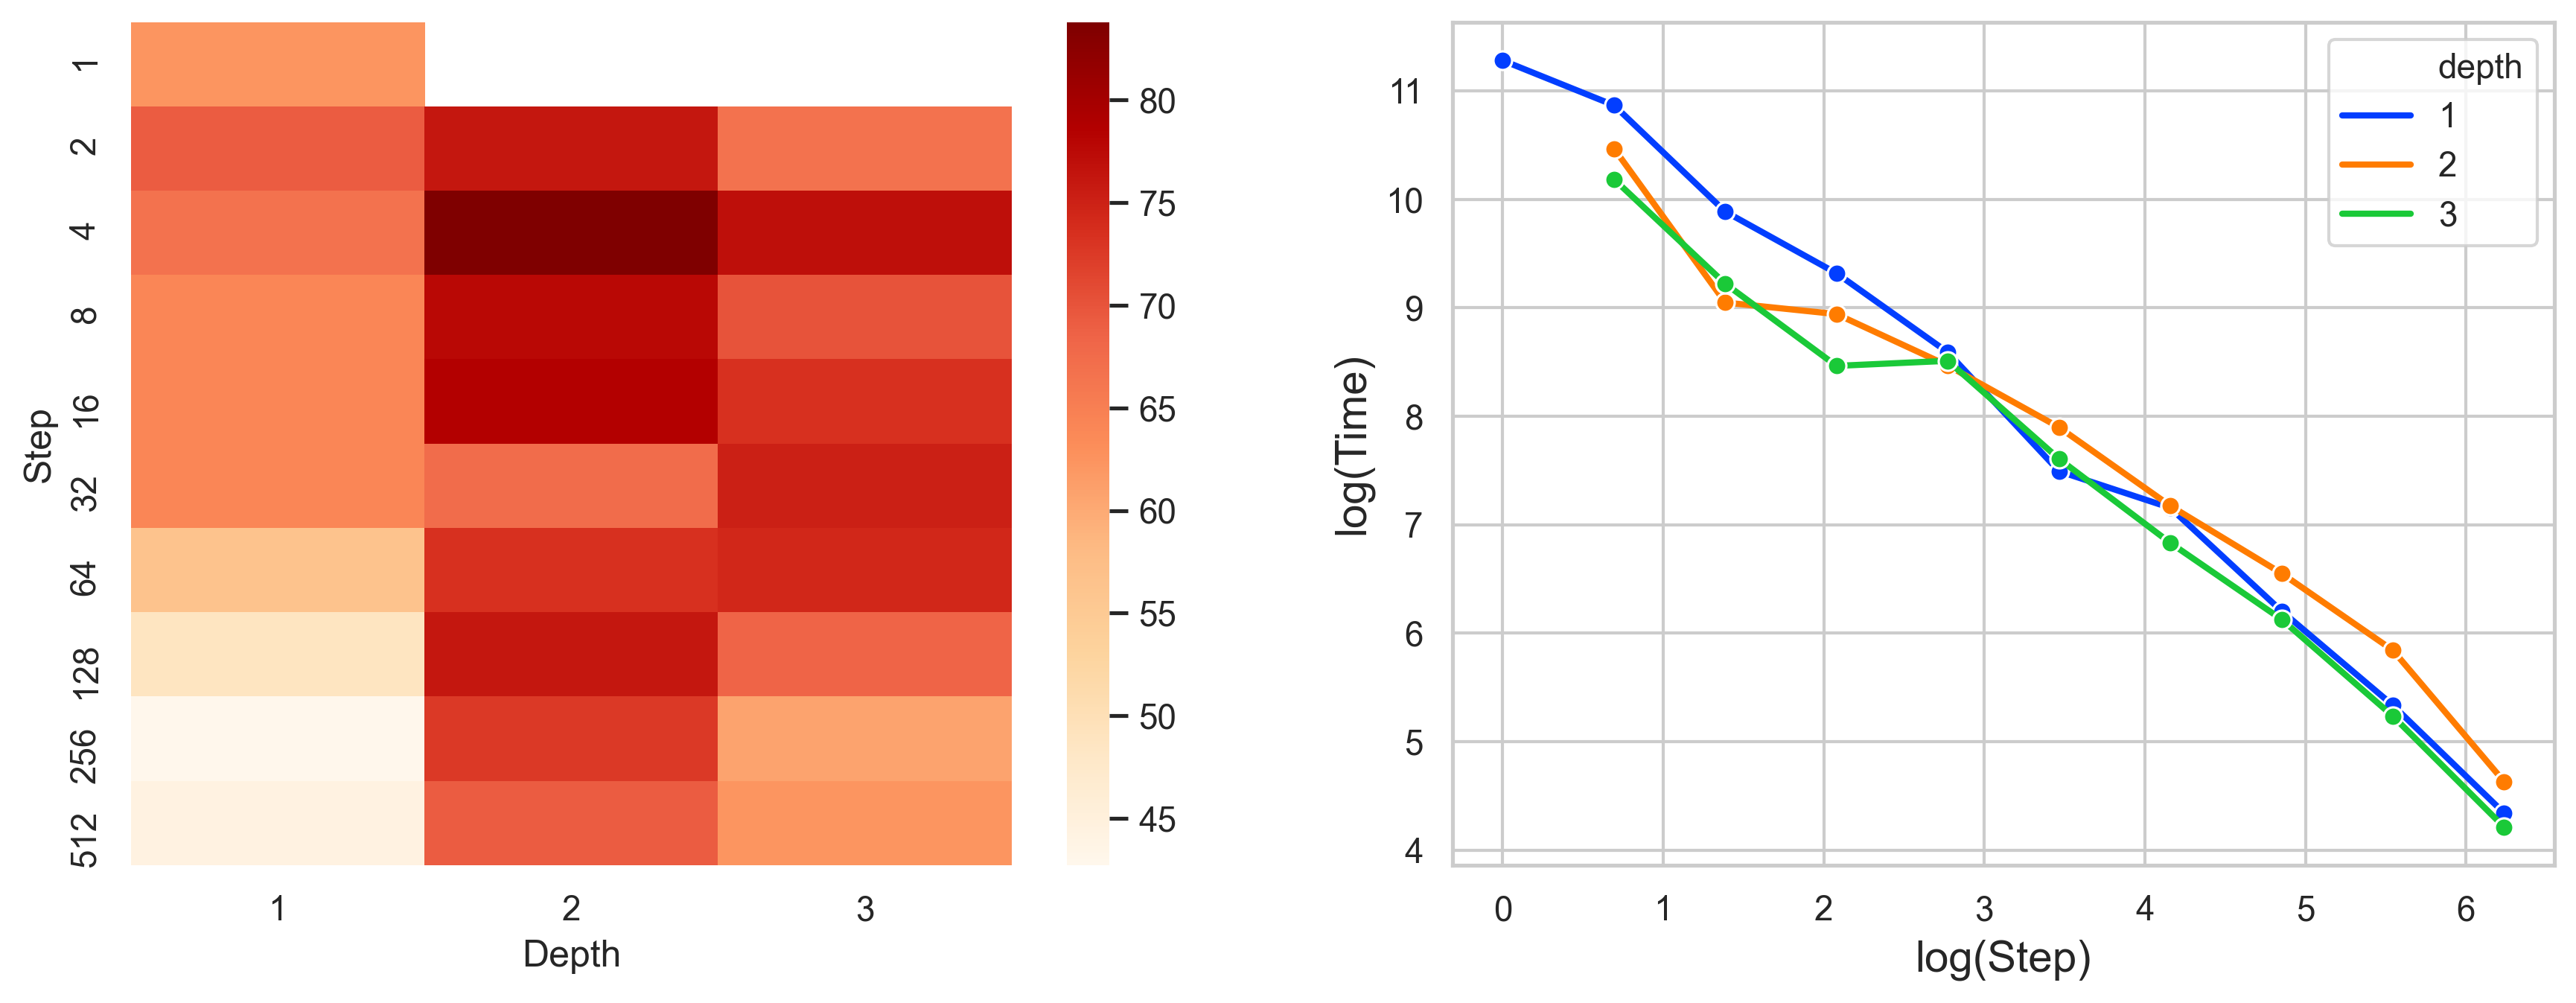
\includegraphics[width=0.95\textwidth]{Images/eigenworms.png}
    \caption{\textbf{Left:} Heatmap of accuracies on the EigenWorms dataset for differing step sizes and depths. \textbf{Right:} Log-log plot of the elapsed time of the algorithm against the step size.}
    \label{fig:eigenworms}
\end{figure}

\begin{table}[t]
    \begin{center}
        \begin{tabular}{ccccc}
        \toprule
        \textbf{Model} & \textbf{Step} & \textbf{Test Accuracy (\%)} & \textbf{Time (Hrs)} & \textbf{Memory (Mb)} \\
        \midrule
        & 1   &  62.4 $\pm$ 12.1 &          22.0 &         176.5 \\
        \multirow{2}{*}{NCDE$_1$}  & 8   &  64.1 $\pm$ 13.3 &           3.1 &          24.3 \\
        & 32  &  64.1 $\pm$ 14.3 &           0.5 &           8.0 \\
        & 128 &   48.7 $\pm$ 2.6 &           0.1 &           3.9 \\
        \midrule
        & 8   &   \textbf{77.8 $\pm$ 5.9} &           2.1 &          94.2 \\
        NCDE$_2$ & 32  &  67.5 $\pm$ 12.1 &           0.7 &          28.1 \\
          & 128 &   \textbf{76.1 $\pm$ 5.9} &           0.2 &           7.8 \\
        \hdashline\noalign{\vskip 0.5ex}
        & 8   &   70.1 $\pm$ 6.5 &           1.3 &         460.7 \\
        NCDE$_3$ & 32  &   \textbf{75.2 $\pm$ 3.0} &           0.6 &         134.7 \\
        & 128 &   68.4 $\pm$ 8.2 &           0.1 &          53.3 \\
        \bottomrule
        \end{tabular}
    \end{center}
    \caption{Performance on the UEA EigenWorms dataset for depths 1-3 and a selection of step sizes. Bold denotes that the model was the top performer for that step-size.}
    \label{tab:eigenworms}
\end{table}

See Table \ref{tab:eigenworms}. We see that the straightforward $\mathrm{NCDE}^1_1$ model takes roughly a day to train. Using the log-ODE method ($\mathrm{NCDE}_2$, $\mathrm{NCDE}_3$) speeds this up to take roughly minutes. Doing so additionally improves model performance dramatically, and reduces memory usage. Naive subsampling approaches ($\mathrm{NCDE}^{8}_1$, $\mathrm{NCDE}^{32}_1$, $\mathrm{NCDE}^{128}_1$) only achieve speedups without performance improvements.

See also Figure \ref{fig:eigenworms}, in which we summarise results for a larger range of step sizes.

\subsection{Estimating Vitals Signs from PPG and ECG Data}
Next we consider the problem of estimating vital signs from PPG and ECG data. The data is taken from the TSR archive \cite{MonashTSRegressionArchive} and involves data from the Beth Israel Deaconess Medical Centre (BIDMC). We consider three tasks whereby we aim to predict a persons respiratory rate (RR), their heart rate (HR), and their oxygen saturation (SpO2). This data is sampled at 125hZ with each series having a length of 4000, 7949 training samples, and a dimension of 3 (including time).

We train a model on each of the three vitals sign prediction tasks using a similar approach to the EigenWorms dataset. The metric used to evaluate performance is the root mean squared error (RMSE) loss which is the standard loss considered in the TSR archive. The results over a range of step sizes are presented in table (\ref{tab:bidmc}). The full results over all step sizes, along with a plots analogous to figure \ref{fig:eigenworms} are left to Appendix \ref{apx:results}.

\begin{table}[t]
    \small
    \begin{center}
        \begin{tabular}{ccccccccc}
        \toprule
        \multirow{2}{*}{\textbf{Depth}} & \multirow{2}{*}{\textbf{Step}} & \multicolumn{3}{c}{\textbf{RMSE}} & \multicolumn{3}{c}{\textbf{Time (H)}} & \multirow{2}{*}{\textbf{Memory (Mb)}} \\
        \cmidrule(lr){3-5} \cmidrule(lr){6-8}
         & & RR & HR & SpO$_2$ & RR & HR & SpO$_2$ & \\
         \midrule
        & 1   &  2.79 $\pm$ 0.04 &   9.82 $\pm$ 0.34 &  2.83 $\pm$ 0.27 &          23.8 &          22.1 &          28.1 &               56.5 \\
        \multirow{2}{*}{NCDE$_1$} & 8   &   2.80 $\pm$ 0.06 &  10.72 $\pm$ 0.24 &  3.43 $\pm$ 0.17 &           3.0 &           2.6 &           4.8 &               14.3 \\
          & 32  &  2.53 $\pm$ 0.23 &  12.23 $\pm$ 0.43 &  2.68 $\pm$ 0.12 &           1.9 &           0.9 &           2.2 &                9.8 \\
          & 128 &  2.64 $\pm$ 0.18 &  11.98 $\pm$ 0.37 &  2.86 $\pm$ 0.04 &           0.2 &           0.2 &           0.3 &                8.7 \\
        \midrule
        & 8   &  2.63 $\pm$ 0.12 &   8.63 $\pm$ 0.24 &  2.88 $\pm$ 0.15 &           2.1 &           3.4 &           3.3 &               21.8 \\
        NCDE$_2$ & 32  &   1.90 $\pm$ 0.02 &     7.90 $\pm$ 1.00 &   1.69 $\pm$ 0.20 &           1.2 &           1.1 &           2.0 &               13.1 \\
          & 128 &  1.86 $\pm$ 0.03 &   6.77 $\pm$ 0.42 &  1.95 $\pm$ 0.18 &           0.3 &           0.4 &           0.7 &               10.9 \\
        \hdashline\noalign{\vskip 0.5ex}
        & 8   &  \textbf{2.42 $\pm$ 0.19} &    \textbf{7.67 $\pm$ 0.40} &  \textbf{2.55 $\pm$ 0.13} &           2.9 &           3.2 &           3.1 &               43.3 \\
        NCDE$_3$ & 32  &  \textbf{1.67 $\pm$ 0.01} &    \textbf{4.50 $\pm$ 0.70} &  \textbf{1.61 $\pm$ 0.05} &           1.3 &           1.8 &           7.3 &               20.5 \\
          & 128 & \textbf{1.51 $\pm$ 0.08} &  \textbf{2.97 $\pm$ 0.45} &  \textbf{1.37 $\pm$ 0.22} &           0.5 &           1.7 &           1.7 &               17.3 \\
        \bottomrule
        \end{tabular}
    \end{center}
    \caption{The RMSE scores on the test set for each of the vitals signs prediction tasks (RR, HR, SpO$_2$) on the BIDMC dataset. The memory usage is given as the mean over all three of the tasks as it was approximately the same for any task for a given depth and step. The bold values denote the algorithm with the lowest test set loss for a fixed step size for each task.}
    \label{tab:bidmc}
\end{table}

We find that the depth $3$ model is the top performer for every task at any step size. Whats more, the top performing depth 3 model from each category also significantly outperforms the NCDE$^1_1$ model with a significantly reduced training time. This again illustrates that the increased step size not only reduces training time, but can also improve model performance. We believe this is attributable to the log-ODE model being better at learning these long-term dependencies, as the worst scores of the NCDE$^s_{2, 3}$ models are with step sizes 2 and 4 for all tasks where they are on par (or worse) than the corresponding depth 1 model.

Both experiments give show that the depth 2 and 3 models can not only reduce training times with similar levels of performance, but can additionally result in improved performance over these large steps. 


\section{Limitations}

\paragraph{Number of hyperparameters} Two new hyperparameters -- truncation depth and step size -- with substantial effects on training time and memory usage must now also be tuned.

\paragraph{Number of input channels} The log-ODE method is most feasible for low numbers of input channels, as the number of logsignature channels $\beta(v, N)$ grows near-exponentially in $v$.

\section{Related Work}
There has been some work on long time series for classic RNN (GRU/LSTM) models. \citet{campos2017skip} introduce the `Skip-RNN' model, which extend the RNN by adding an additional learnt component that skips state updates. This reduces the number of computations in the forward pass. However, this model is now not dependent on the within-skip input data. Furthermore, one does not know a priori how many states the model will choose to skip, which can lead to memory difficulties. 

Another approach is hierarchical subsampling as in \citet{graves2012supervised, de2015survey}, which operates over multiple training examples at a time as an input, thus reducing the number of total forward computations. Whilst this method is dependent on all the data, it naively uses the raw data when an appropriate summarisation would be more sensible.

This is rectified in \cite{liao2019learning} where the authors in fact use the logsignature as their summarisation procedure.


However, as is common with all of these models, it describes some some modification of the RNN structure but it has been shown in \cite{kidger2020neural} that the NCDE model subsumes the class of RNN/LSTM/GRU, in that it can model a wider class of functions. Additionally, none of these approaches be solved using ODE methods and thus are not able to utilise the adjoint method, continuous time dynamics, and so on.   


\section{Conclusions}
We have shown how the integral equation from the Neural CDE model can be solved with high accuracy over intervals larger than the discretisation of the data can be solved using the log-ODE method. We demonstrated that this not only enables us to take longer steps over the data whilst retaining model performance resulting in significantly lower training times, but also that this can result in models that achieve better performance over large step sizes than the original model over any step size, including updating the hidden state at every data point. 




\subsubsection*{Author Contributions}


\subsubsection*{Acknowledgements}
JM was supported by the EPSRC grant EP/L015803/1 in collaboration
with Iterex Therapuetics. CS was supported by the
EPSRC grant EP/R513295/1. PK was supported by the EPSRC grant EP/L015811/1. JF was supported by the EPSRC grant EP/N509711/1. JM, CS, PK, JF, TL were supported by the Alan Turing Institute under the EPSRC grant EP/N510129/1.


\bibliography{bibliography}
\bibliographystyle{style/iclr2020_conference}

\newpage

\documentclass{article} % For LaTeX2e
\usepackage{style/iclr2020_conference,times}

% Optional math commands from https://github.com/goodfeli/dlbook_notation.
%%%%% NEW MATH DEFINITIONS %%%%%

\usepackage{amsmath,amsfonts,bm}

% Mark sections of captions for referring to divisions of figures
\newcommand{\figleft}{{\em (Left)}}
\newcommand{\figcenter}{{\em (Center)}}
\newcommand{\figright}{{\em (Right)}}
\newcommand{\figtop}{{\em (Top)}}
\newcommand{\figbottom}{{\em (Bottom)}}
\newcommand{\captiona}{{\em (a)}}
\newcommand{\captionb}{{\em (b)}}
\newcommand{\captionc}{{\em (c)}}
\newcommand{\captiond}{{\em (d)}}

% Highlight a newly defined term
\newcommand{\newterm}[1]{{\bf #1}}


% Figure reference, lower-case.
\def\figref#1{figure~\ref{#1}}
% Figure reference, capital. For start of sentence
\def\Figref#1{Figure~\ref{#1}}
\def\twofigref#1#2{figures \ref{#1} and \ref{#2}}
\def\quadfigref#1#2#3#4{figures \ref{#1}, \ref{#2}, \ref{#3} and \ref{#4}}
% Section reference, lower-case.
\def\secref#1{section~\ref{#1}}
% Section reference, capital.
\def\Secref#1{Section~\ref{#1}}
% Reference to two sections.
\def\twosecrefs#1#2{sections \ref{#1} and \ref{#2}}
% Reference to three sections.
\def\secrefs#1#2#3{sections \ref{#1}, \ref{#2} and \ref{#3}}
% Reference to an equation, lower-case.
\def\eqref#1{equation~\ref{#1}}
% Reference to an equation, upper case
\def\Eqref#1{Equation~\ref{#1}}
% A raw reference to an equation---avoid using if possible
\def\plaineqref#1{\ref{#1}}
% Reference to a chapter, lower-case.
\def\chapref#1{chapter~\ref{#1}}
% Reference to an equation, upper case.
\def\Chapref#1{Chapter~\ref{#1}}
% Reference to a range of chapters
\def\rangechapref#1#2{chapters\ref{#1}--\ref{#2}}
% Reference to an algorithm, lower-case.
\def\algref#1{algorithm~\ref{#1}}
% Reference to an algorithm, upper case.
\def\Algref#1{Algorithm~\ref{#1}}
\def\twoalgref#1#2{algorithms \ref{#1} and \ref{#2}}
\def\Twoalgref#1#2{Algorithms \ref{#1} and \ref{#2}}
% Reference to a part, lower case
\def\partref#1{part~\ref{#1}}
% Reference to a part, upper case
\def\Partref#1{Part~\ref{#1}}
\def\twopartref#1#2{parts \ref{#1} and \ref{#2}}

\def\ceil#1{\lceil #1 \rceil}
\def\floor#1{\lfloor #1 \rfloor}
\def\1{\bm{1}}
\newcommand{\train}{\mathcal{D}}
\newcommand{\valid}{\mathcal{D_{\mathrm{valid}}}}
\newcommand{\test}{\mathcal{D_{\mathrm{test}}}}

\def\eps{{\epsilon}}


% Random variables
\def\reta{{\textnormal{$\eta$}}}
\def\ra{{\textnormal{a}}}
\def\rb{{\textnormal{b}}}
\def\rc{{\textnormal{c}}}
\def\rd{{\textnormal{d}}}
\def\re{{\textnormal{e}}}
\def\rf{{\textnormal{f}}}
\def\rg{{\textnormal{g}}}
\def\rh{{\textnormal{h}}}
\def\ri{{\textnormal{i}}}
\def\rj{{\textnormal{j}}}
\def\rk{{\textnormal{k}}}
\def\rl{{\textnormal{l}}}
% rm is already a command, just don't name any random variables m
\def\rn{{\textnormal{n}}}
\def\ro{{\textnormal{o}}}
\def\rp{{\textnormal{p}}}
\def\rq{{\textnormal{q}}}
\def\rr{{\textnormal{r}}}
\def\rs{{\textnormal{s}}}
\def\rt{{\textnormal{t}}}
\def\ru{{\textnormal{u}}}
\def\rv{{\textnormal{v}}}
\def\rw{{\textnormal{w}}}
\def\rx{{\textnormal{x}}}
\def\ry{{\textnormal{y}}}
\def\rz{{\textnormal{z}}}

% Random vectors
\def\rvepsilon{{\mathbf{\epsilon}}}
\def\rvtheta{{\mathbf{\theta}}}
\def\rva{{\mathbf{a}}}
\def\rvb{{\mathbf{b}}}
\def\rvc{{\mathbf{c}}}
\def\rvd{{\mathbf{d}}}
\def\rve{{\mathbf{e}}}
\def\rvf{{\mathbf{f}}}
\def\rvg{{\mathbf{g}}}
\def\rvh{{\mathbf{h}}}
\def\rvu{{\mathbf{i}}}
\def\rvj{{\mathbf{j}}}
\def\rvk{{\mathbf{k}}}
\def\rvl{{\mathbf{l}}}
\def\rvm{{\mathbf{m}}}
\def\rvn{{\mathbf{n}}}
\def\rvo{{\mathbf{o}}}
\def\rvp{{\mathbf{p}}}
\def\rvq{{\mathbf{q}}}
\def\rvr{{\mathbf{r}}}
\def\rvs{{\mathbf{s}}}
\def\rvt{{\mathbf{t}}}
\def\rvu{{\mathbf{u}}}
\def\rvv{{\mathbf{v}}}
\def\rvw{{\mathbf{w}}}
\def\rvx{{\mathbf{x}}}
\def\rvy{{\mathbf{y}}}
\def\rvz{{\mathbf{z}}}

% Elements of random vectors
\def\erva{{\textnormal{a}}}
\def\ervb{{\textnormal{b}}}
\def\ervc{{\textnormal{c}}}
\def\ervd{{\textnormal{d}}}
\def\erve{{\textnormal{e}}}
\def\ervf{{\textnormal{f}}}
\def\ervg{{\textnormal{g}}}
\def\ervh{{\textnormal{h}}}
\def\ervi{{\textnormal{i}}}
\def\ervj{{\textnormal{j}}}
\def\ervk{{\textnormal{k}}}
\def\ervl{{\textnormal{l}}}
\def\ervm{{\textnormal{m}}}
\def\ervn{{\textnormal{n}}}
\def\ervo{{\textnormal{o}}}
\def\ervp{{\textnormal{p}}}
\def\ervq{{\textnormal{q}}}
\def\ervr{{\textnormal{r}}}
\def\ervs{{\textnormal{s}}}
\def\ervt{{\textnormal{t}}}
\def\ervu{{\textnormal{u}}}
\def\ervv{{\textnormal{v}}}
\def\ervw{{\textnormal{w}}}
\def\ervx{{\textnormal{x}}}
\def\ervy{{\textnormal{y}}}
\def\ervz{{\textnormal{z}}}

% Random matrices
\def\rmA{{\mathbf{A}}}
\def\rmB{{\mathbf{B}}}
\def\rmC{{\mathbf{C}}}
\def\rmD{{\mathbf{D}}}
\def\rmE{{\mathbf{E}}}
\def\rmF{{\mathbf{F}}}
\def\rmG{{\mathbf{G}}}
\def\rmH{{\mathbf{H}}}
\def\rmI{{\mathbf{I}}}
\def\rmJ{{\mathbf{J}}}
\def\rmK{{\mathbf{K}}}
\def\rmL{{\mathbf{L}}}
\def\rmM{{\mathbf{M}}}
\def\rmN{{\mathbf{N}}}
\def\rmO{{\mathbf{O}}}
\def\rmP{{\mathbf{P}}}
\def\rmQ{{\mathbf{Q}}}
\def\rmR{{\mathbf{R}}}
\def\rmS{{\mathbf{S}}}
\def\rmT{{\mathbf{T}}}
\def\rmU{{\mathbf{U}}}
\def\rmV{{\mathbf{V}}}
\def\rmW{{\mathbf{W}}}
\def\rmX{{\mathbf{X}}}
\def\rmY{{\mathbf{Y}}}
\def\rmZ{{\mathbf{Z}}}

% Elements of random matrices
\def\ermA{{\textnormal{A}}}
\def\ermB{{\textnormal{B}}}
\def\ermC{{\textnormal{C}}}
\def\ermD{{\textnormal{D}}}
\def\ermE{{\textnormal{E}}}
\def\ermF{{\textnormal{F}}}
\def\ermG{{\textnormal{G}}}
\def\ermH{{\textnormal{H}}}
\def\ermI{{\textnormal{I}}}
\def\ermJ{{\textnormal{J}}}
\def\ermK{{\textnormal{K}}}
\def\ermL{{\textnormal{L}}}
\def\ermM{{\textnormal{M}}}
\def\ermN{{\textnormal{N}}}
\def\ermO{{\textnormal{O}}}
\def\ermP{{\textnormal{P}}}
\def\ermQ{{\textnormal{Q}}}
\def\ermR{{\textnormal{R}}}
\def\ermS{{\textnormal{S}}}
\def\ermT{{\textnormal{T}}}
\def\ermU{{\textnormal{U}}}
\def\ermV{{\textnormal{V}}}
\def\ermW{{\textnormal{W}}}
\def\ermX{{\textnormal{X}}}
\def\ermY{{\textnormal{Y}}}
\def\ermZ{{\textnormal{Z}}}

% Vectors
\def\vzero{{\bm{0}}}
\def\vone{{\bm{1}}}
\def\vmu{{\bm{\mu}}}
\def\vtheta{{\bm{\theta}}}
\def\va{{\bm{a}}}
\def\vb{{\bm{b}}}
\def\vc{{\bm{c}}}
\def\vd{{\bm{d}}}
\def\ve{{\bm{e}}}
\def\vf{{\bm{f}}}
\def\vg{{\bm{g}}}
\def\vh{{\bm{h}}}
\def\vi{{\bm{i}}}
\def\vj{{\bm{j}}}
\def\vk{{\bm{k}}}
\def\vl{{\bm{l}}}
\def\vm{{\bm{m}}}
\def\vn{{\bm{n}}}
\def\vo{{\bm{o}}}
\def\vp{{\bm{p}}}
\def\vq{{\bm{q}}}
\def\vr{{\bm{r}}}
\def\vs{{\bm{s}}}
\def\vt{{\bm{t}}}
\def\vu{{\bm{u}}}
\def\vv{{\bm{v}}}
\def\vw{{\bm{w}}}
\def\vx{{\bm{x}}}
\def\vy{{\bm{y}}}
\def\vz{{\bm{z}}}

% Elements of vectors
\def\evalpha{{\alpha}}
\def\evbeta{{\beta}}
\def\evepsilon{{\epsilon}}
\def\evlambda{{\lambda}}
\def\evomega{{\omega}}
\def\evmu{{\mu}}
\def\evpsi{{\psi}}
\def\evsigma{{\sigma}}
\def\evtheta{{\theta}}
\def\eva{{a}}
\def\evb{{b}}
\def\evc{{c}}
\def\evd{{d}}
\def\eve{{e}}
\def\evf{{f}}
\def\evg{{g}}
\def\evh{{h}}
\def\evi{{i}}
\def\evj{{j}}
\def\evk{{k}}
\def\evl{{l}}
\def\evm{{m}}
\def\evn{{n}}
\def\evo{{o}}
\def\evp{{p}}
\def\evq{{q}}
\def\evr{{r}}
\def\evs{{s}}
\def\evt{{t}}
\def\evu{{u}}
\def\evv{{v}}
\def\evw{{w}}
\def\evx{{x}}
\def\evy{{y}}
\def\evz{{z}}

% Matrix
\def\mA{{\bm{A}}}
\def\mB{{\bm{B}}}
\def\mC{{\bm{C}}}
\def\mD{{\bm{D}}}
\def\mE{{\bm{E}}}
\def\mF{{\bm{F}}}
\def\mG{{\bm{G}}}
\def\mH{{\bm{H}}}
\def\mI{{\bm{I}}}
\def\mJ{{\bm{J}}}
\def\mK{{\bm{K}}}
\def\mL{{\bm{L}}}
\def\mM{{\bm{M}}}
\def\mN{{\bm{N}}}
\def\mO{{\bm{O}}}
\def\mP{{\bm{P}}}
\def\mQ{{\bm{Q}}}
\def\mR{{\bm{R}}}
\def\mS{{\bm{S}}}
\def\mT{{\bm{T}}}
\def\mU{{\bm{U}}}
\def\mV{{\bm{V}}}
\def\mW{{\bm{W}}}
\def\mX{{\bm{X}}}
\def\mY{{\bm{Y}}}
\def\mZ{{\bm{Z}}}
\def\mBeta{{\bm{\beta}}}
\def\mPhi{{\bm{\Phi}}}
\def\mLambda{{\bm{\Lambda}}}
\def\mSigma{{\bm{\Sigma}}}

% Tensor
\DeclareMathAlphabet{\mathsfit}{\encodingdefault}{\sfdefault}{m}{sl}
\SetMathAlphabet{\mathsfit}{bold}{\encodingdefault}{\sfdefault}{bx}{n}
\newcommand{\tens}[1]{\bm{\mathsfit{#1}}}
\def\tA{{\tens{A}}}
\def\tB{{\tens{B}}}
\def\tC{{\tens{C}}}
\def\tD{{\tens{D}}}
\def\tE{{\tens{E}}}
\def\tF{{\tens{F}}}
\def\tG{{\tens{G}}}
\def\tH{{\tens{H}}}
\def\tI{{\tens{I}}}
\def\tJ{{\tens{J}}}
\def\tK{{\tens{K}}}
\def\tL{{\tens{L}}}
\def\tM{{\tens{M}}}
\def\tN{{\tens{N}}}
\def\tO{{\tens{O}}}
\def\tP{{\tens{P}}}
\def\tQ{{\tens{Q}}}
\def\tR{{\tens{R}}}
\def\tS{{\tens{S}}}
\def\tT{{\tens{T}}}
\def\tU{{\tens{U}}}
\def\tV{{\tens{V}}}
\def\tW{{\tens{W}}}
\def\tX{{\tens{X}}}
\def\tY{{\tens{Y}}}
\def\tZ{{\tens{Z}}}


% Graph
\def\gA{{\mathcal{A}}}
\def\gB{{\mathcal{B}}}
\def\gC{{\mathcal{C}}}
\def\gD{{\mathcal{D}}}
\def\gE{{\mathcal{E}}}
\def\gF{{\mathcal{F}}}
\def\gG{{\mathcal{G}}}
\def\gH{{\mathcal{H}}}
\def\gI{{\mathcal{I}}}
\def\gJ{{\mathcal{J}}}
\def\gK{{\mathcal{K}}}
\def\gL{{\mathcal{L}}}
\def\gM{{\mathcal{M}}}
\def\gN{{\mathcal{N}}}
\def\gO{{\mathcal{O}}}
\def\gP{{\mathcal{P}}}
\def\gQ{{\mathcal{Q}}}
\def\gR{{\mathcal{R}}}
\def\gS{{\mathcal{S}}}
\def\gT{{\mathcal{T}}}
\def\gU{{\mathcal{U}}}
\def\gV{{\mathcal{V}}}
\def\gW{{\mathcal{W}}}
\def\gX{{\mathcal{X}}}
\def\gY{{\mathcal{Y}}}
\def\gZ{{\mathcal{Z}}}

% Sets
\def\sA{{\mathbb{A}}}
\def\sB{{\mathbb{B}}}
\def\sC{{\mathbb{C}}}
\def\sD{{\mathbb{D}}}
% Don't use a set called E, because this would be the same as our symbol
% for expectation.
\def\sF{{\mathbb{F}}}
\def\sG{{\mathbb{G}}}
\def\sH{{\mathbb{H}}}
\def\sI{{\mathbb{I}}}
\def\sJ{{\mathbb{J}}}
\def\sK{{\mathbb{K}}}
\def\sL{{\mathbb{L}}}
\def\sM{{\mathbb{M}}}
\def\sN{{\mathbb{N}}}
\def\sO{{\mathbb{O}}}
\def\sP{{\mathbb{P}}}
\def\sQ{{\mathbb{Q}}}
\def\sR{{\mathbb{R}}}
\def\sS{{\mathbb{S}}}
\def\sT{{\mathbb{T}}}
\def\sU{{\mathbb{U}}}
\def\sV{{\mathbb{V}}}
\def\sW{{\mathbb{W}}}
\def\sX{{\mathbb{X}}}
\def\sY{{\mathbb{Y}}}
\def\sZ{{\mathbb{Z}}}

% Entries of a matrix
\def\emLambda{{\Lambda}}
\def\emA{{A}}
\def\emB{{B}}
\def\emC{{C}}
\def\emD{{D}}
\def\emE{{E}}
\def\emF{{F}}
\def\emG{{G}}
\def\emH{{H}}
\def\emI{{I}}
\def\emJ{{J}}
\def\emK{{K}}
\def\emL{{L}}
\def\emM{{M}}
\def\emN{{N}}
\def\emO{{O}}
\def\emP{{P}}
\def\emQ{{Q}}
\def\emR{{R}}
\def\emS{{S}}
\def\emT{{T}}
\def\emU{{U}}
\def\emV{{V}}
\def\emW{{W}}
\def\emX{{X}}
\def\emY{{Y}}
\def\emZ{{Z}}
\def\emSigma{{\Sigma}}

% entries of a tensor
% Same font as tensor, without \bm wrapper
\newcommand{\etens}[1]{\mathsfit{#1}}
\def\etLambda{{\etens{\Lambda}}}
\def\etA{{\etens{A}}}
\def\etB{{\etens{B}}}
\def\etC{{\etens{C}}}
\def\etD{{\etens{D}}}
\def\etE{{\etens{E}}}
\def\etF{{\etens{F}}}
\def\etG{{\etens{G}}}
\def\etH{{\etens{H}}}
\def\etI{{\etens{I}}}
\def\etJ{{\etens{J}}}
\def\etK{{\etens{K}}}
\def\etL{{\etens{L}}}
\def\etM{{\etens{M}}}
\def\etN{{\etens{N}}}
\def\etO{{\etens{O}}}
\def\etP{{\etens{P}}}
\def\etQ{{\etens{Q}}}
\def\etR{{\etens{R}}}
\def\etS{{\etens{S}}}
\def\etT{{\etens{T}}}
\def\etU{{\etens{U}}}
\def\etV{{\etens{V}}}
\def\etW{{\etens{W}}}
\def\etX{{\etens{X}}}
\def\etY{{\etens{Y}}}
\def\etZ{{\etens{Z}}}

% The true underlying data generating distribution
\newcommand{\pdata}{p_{\rm{data}}}
% The empirical distribution defined by the training set
\newcommand{\ptrain}{\hat{p}_{\rm{data}}}
\newcommand{\Ptrain}{\hat{P}_{\rm{data}}}
% The model distribution
\newcommand{\pmodel}{p_{\rm{model}}}
\newcommand{\Pmodel}{P_{\rm{model}}}
\newcommand{\ptildemodel}{\tilde{p}_{\rm{model}}}
% Stochastic autoencoder distributions
\newcommand{\pencode}{p_{\rm{encoder}}}
\newcommand{\pdecode}{p_{\rm{decoder}}}
\newcommand{\precons}{p_{\rm{reconstruct}}}

\newcommand{\laplace}{\mathrm{Laplace}} % Laplace distribution

\newcommand{\E}{\mathbb{E}}
\newcommand{\Ls}{\mathcal{L}}
\newcommand{\R}{\mathbb{R}}
\newcommand{\emp}{\tilde{p}}
\newcommand{\lr}{\alpha}
\newcommand{\reg}{\lambda}
\newcommand{\rect}{\mathrm{rectifier}}
\newcommand{\softmax}{\mathrm{softmax}}
\newcommand{\sigmoid}{\sigma}
\newcommand{\softplus}{\zeta}
\newcommand{\KL}{D_{\mathrm{KL}}}
\newcommand{\Var}{\mathrm{Var}}
\newcommand{\standarderror}{\mathrm{SE}}
\newcommand{\Cov}{\mathrm{Cov}}
\newcommand{\m}{\hspace{0.25mm}}
\newcommand{\mm}{\hspace{5mm}}
\newcommand{\D}{\mathcal{D}}
% Wolfram Mathworld says $L^2$ is for function spaces and $\ell^2$ is for vectors
% But then they seem to use $L^2$ for vectors throughout the site, and so does
% wikipedia.
\newcommand{\normlzero}{L^0}
\newcommand{\normlone}{L^1}
\newcommand{\normltwo}{L^2}
\newcommand{\normlp}{L^p}
\newcommand{\normmax}{L^\infty}
\newcommand{\parents}{Pa} % See usage in notation.tex. Chosen to match Daphne's book.

\DeclareMathOperator*{\argmax}{arg\,max}
\DeclareMathOperator*{\argmin}{arg\,min}

\DeclareMathOperator{\sign}{sign}
\DeclareMathOperator{\Tr}{Tr}
\let\ab\allowbreak


\usepackage{hyperref}
\usepackage{url}

\usepackage{booktabs}       % professional-quality tables
\usepackage{arydshln}
\usepackage{amssymb}
\setlength\dashlinegap{2.5pt}

\usepackage{graphicx}
\usepackage{subcaption}
\usepackage{rotating}
\usepackage{ifthen}
\graphicspath{ {Images/} }

\newtheorem{theorem}{Theorem}[section]
\newtheorem{lemma}[theorem]{Lemma}
\newtheorem{prop}[theorem]{Proposition}
\newtheorem{proof}[theorem]{Proof}
\newtheorem{corollary}[theorem]{Corollary}
\newtheorem{method}[theorem]{Method}
\newtheorem{definition}[theorem]{Definition}
\newtheorem{example}[theorem]{Example}
\newtheorem{xca}[theorem]{Exercise}
\newtheorem{remark}[theorem]{Remark}

% This file contains lots of tikz stuff
% Tikz
\usepackage{ifthen}
\usepackage{intcalc}
\usepackage{tikz}
\usepackage{multirow}
\usetikzlibrary{decorations.pathreplacing,calligraphy}
\usetikzlibrary{arrows.meta, decorations.text, decorations.markings, decorations.pathreplacing, angles, quotes, calligraphy}
\definecolor{bittersweet}{rgb}{1.0, 0.44, 0.37}

% Logisig definitions
% Log-sig heights
\pgfmathsetmacro{\pathyshift}{0.8}
\global\def\rs{{0, 1, 2.1, 3.3, 4.5, 5.5, 6.5}}
\global\def\lsone{{2.15, 2.3, 2.1, 2.4, 2.1, 2.4}}
\global\def\lstwo{{2.1, 2.4, 2.2, 2.5, 2.2, 2.1}}
\global\def\lsthree{{2.3, 2.1, 2.15, 2.35, 2.5, 2.2}}
\global\def\lspathraise{0.7}
\global\def\data{{0.4, 0.7, 0.9, 0.5, 0.6, 0.9, 0.8, 0.5, 0.3, 0.3, 0.8, 1.0, 0.2, 0.4, 0.7, 0.5, 1.0, 1.0, 0.8, 0.4, 0.2, 0.6, 0.8, 0.5, 0.3, 0.5, 0.2, 0.1, 0.5, 0.2, 0.4, 0.6, 0.3, 0.2, 0.1, 0.7, 0.6, 0.2, 0.5, 0.4, 0.4, 0.1}}

% Logsig
\definecolor{colorls1}{HTML}{66C2A5}
\definecolor{colorls2}{HTML}{8DA0CB}
\definecolor{colorls3}{HTML}{FC8D62}

\newcommand\ncdediagram[1]{
    \begin{tikzpicture}
        % Choose between the logsig and normal version
        \pgfmathsetmacro{\logsigversion}{#1}
        
        % For reducing the height of the hidden state and integration steps in the two cases
        \ifthenelse{\logsigversion=0}
            {\pgfmathsetmacro{\hreduce}{1.8}}
            {\pgfmathsetmacro{\hreduce}{0}}
        
        % Time
        \draw[black, thick, ->] (0, 0) -- (7, 0);
        
        \ifthenelse{\logsigversion=0}
            {
                \foreach \i in {0, 6} {
                    \node at (\rs[\i], 0)[circle,fill, inner sep=1.5pt] {};
                }
                \node at (\rs[0], -0.25) {\tiny $t_0$};
                \node at (\rs[6], -0.25) {\tiny $t_m$};
            }
            {
                \foreach \i in {0, 1, 2, 3, 4, 5, 6} {
                    \node at (\rs[\i], 0)[circle,fill, inner sep=1.5pt] {};
                }
                \node at (\rs[0], -0.25) {\tiny $r_0$};
                \node at (\rs[1], -0.25) {\tiny $r_1$};
                \node at (\rs[2], -0.25) {\tiny $r_2$};
                \node at (\rs[3], -0.25) {\tiny $r_3$};
                \node at (\rs[4], -0.25) {\tiny $r_{m-2}$};
                \node at (\rs[5], -0.25) {\tiny $r_{m-1}$};
                \node at (\rs[6], -0.25) {\tiny $r_m$};
            }
        \node at (3.85, -0.25) {\tiny $\cdots$};
    
        
    
        
        \pgfmathsetmacro{\dataix}{0}
        \pgfmathsetmacro{\midwayprev}{0}
        \pgfmathsetmacro{\xprev}{0}
        \pgfmathsetmacro{\yprev}{0}
        \foreach \i in {0, 1, 2, 3, 4, 5} {
            % Macros
            \pgfmathsetmacro{\frac}{\rs[\i + 1] - \rs[\i]}
            \pgfmathsetmacro{\midway}{\rs[\i] + (\rs[\i + 1] - \rs[\i]) * 0.5}
            
            % Data and path
            \foreach \d in {0, 1, 2, 3, 4, 5, 6} {
                \ifthenelse{\i>0 \AND \d=0}{\pgfmathsetmacro{\y}{\data[\dataix - 1] * 0.5 + 0.1}}{\pgfmathsetmacro{\y}{\data[\dataix] * 0.5 + 0.1}}
                \pgfmathsetmacro{\x}{\rs[\i] + \d * \frac * 0.1667}
                \pgfmathsetmacro{\dx}{\frac * 0.1667}
                \ifthenelse{\i=3}
                    {
                        % Data
                        \node at (\x, \y)[circle, draw=black, fill=green!50, inner sep=1.5pt, opacity=0.3] {};
                        % Path
                        \node at (\x, \y + \pathyshift)[circle, draw=black, fill=green!50, inner sep=0.5pt, densely dashed] {};
                        \draw[green!50, thick, cap=round, dashed] (\xprev, \yprev + \pathyshift) -- (\x, \y + \pathyshift);
                    }
                    {
                        % Time tick
                        \ifthenelse{\logsigversion=0}{\draw (\x, -0.05) -- (\x, 0.05);}{}
                        % Data
                        \node at (\x, \y)[circle, draw=black, fill=green!50, inner sep=1.5pt] {};
                        % Path
                        \node at (\x, \y + \pathyshift)[circle, draw=black, fill=green!50, inner sep=0.5pt] {};
                        \ifthenelse{\i=0 \AND \d=0}{}{\draw[green!50, thick, cap=round] (\xprev, \yprev + \pathyshift) -- (\x, \y + \pathyshift);}
                        % Integration steps
                        \ifthenelse{\logsigversion=0}
                            {
                                \ifthenelse{\d=6 \AND \i=5}
                                    {}
                                    {
                                        \node at (\x, 3.8 - \hreduce)[circle, draw=black, fill=orange!50, inner sep=1.5pt] {};
                                    }
                            }
                            {}
                    }
                % Update globals
                \pgfmathsetmacro{\dataixnew}{\dataix + 1}
                \global\let\dataix=\dataixnew
                \global\let\yprev=\y
                \global\let\xprev=\x
                
            }
            
            \ifthenelse{\logsigversion=1}{
                \ifthenelse{\i=3}
                    {
                        % Integration steps
                        \node at (\rs[\i], 3.8)[circle, draw=black, fill=orange!50, inner sep=1.5pt] {};
                        \draw[->, dashed] (\rs[\i] + 0.08, 3.8) -- (\rs[\i+1] - 0.08, 3.8);
                        % % Brace
                        % \draw[decoration={calligraphic brace, amplitude=3pt}, decorate, line width=1pt, dotted] (\rs[\i] + 0.05, 1.65) node {} -- (\rs[\i+1] - 0.05, 1.65);
                        % % Brace arrow
                        % \draw[->, dashed] (\midway, 1.8) -- (\midway, 2.0);
                        % % Log-signatures
                        % \node at (\midway, \lsone[\i])[circle, draw=black, fill=colorls1, inner sep=1pt, opacity=0.3] {};
                        % \node at (\midway, \lstwo[\i])[circle, draw=black, fill=colorls2, inner sep=1pt, opacity=0.3] {};
                        % \node at (\midway, \lsthree[\i])[circle, draw=black, fill=colorls3, inner sep=1pt, opacity=0.3] {};
                    }
                    {
                        % Brace
                        \draw[decoration={calligraphic brace, amplitude=3pt}, decorate, line width=1pt] (\rs[\i] + 0.05, 1.65) node {} -- (\rs[\i+1] - 0.05, 1.65);
                        % Brace arrow
                        \draw[->, dashed] (\midway, 1.8) -- (\midway, 2.0);
                        % Log-signatures
                        \node at (\midway, \lsone[\i])[circle, draw=black, fill=colorls1, inner sep=1pt] {};
                        \node at (\midway, \lstwo[\i])[circle, draw=black, fill=colorls2, inner sep=1pt] {};
                        \node at (\midway, \lsthree[\i])[circle, draw=black, fill=colorls3, inner sep=1pt] {};
                        % Integration steps
                        \node at (\rs[\i], 3.8)[circle, draw=black, fill=orange!50, inner sep=1.5pt] {};
                        \draw[->] (\rs[\i] + 0.08, 3.8) -- (\rs[\i+1] - 0.08, 3.8);
                    }
                % Path raise
                \ifthenelse{\i=3}
                    {
                        
                    }
                    {
                        \node at (\midway, \lsone[\i] + \lspathraise)[circle, draw=black, fill=colorls1, inner sep=.5pt] {};
                        \node at (\midway, \lstwo[\i] + \lspathraise)[circle, draw=black, fill=colorls2, inner sep=.5pt] {};
                        \node at (\midway, \lsthree[\i] + \lspathraise)[circle, draw=black, fill=colorls3, inner sep=.5pt] {};
                    }
                % Log-sig path
                \ifthenelse{\i>0}
                    {   
                        % Horrendous code to dash out the middle logsig bit
                        \ifthenelse{\i=3 \OR \i=4}
                        {  
                            \ifthenelse{\i=3}
                                {
                                    \pgfmathsetmacro{\midmidway}{\midwayprev + (\midway - \midwayprev) * 0.5}
                                    \draw[colorls1, thick, cap=round] (\midwayprev, \lsone[\i-1] + \lspathraise) -- (\midmidway, \lsone[\i-1]*0.5 + \lsone[\i]*0.5 + \lspathraise);
                                    \draw[colorls1, thick, cap=round, densely dashed] (\midmidway, \lsone[\i-1]*0.5 + \lsone[\i]*0.5 + \lspathraise) -- (\midway, \lsone[\i] + \lspathraise);
                                    \draw[colorls2, thick, cap=round] (\midwayprev, \lstwo[\i-1] + \lspathraise) -- (\midmidway, \lstwo[\i-1]*0.5 + \lstwo[\i]*0.5 + \lspathraise);
                                    \draw[colorls2, thick, cap=round, densely dashed] (\midmidway, \lstwo[\i-1]*0.5 + \lstwo[\i]*0.5 + \lspathraise) -- (\midway, \lstwo[\i] + \lspathraise);
                                    \draw[colorls3, thick, cap=round] (\midwayprev, \lsthree[\i-1] + \lspathraise) -- (\midmidway, \lsthree[\i-1]*0.5 + \lsthree[\i]*0.5 + \lspathraise);
                                    \draw[colorls3, thick, cap=round, densely dashed] (\midmidway, \lsthree[\i-1]*0.5 + \lsthree[\i]*0.5 + \lspathraise) -- (\midway, \lsthree[\i] + \lspathraise);
                                }
                                {
                                    \pgfmathsetmacro{\midmidway}{\midwayprev + (\midway - \midwayprev) * 0.5}
                                    \draw[colorls1, thick, cap=round, densely dashed] (\midwayprev, \lsone[\i-1] + \lspathraise) -- (\midmidway, \lsone[\i-1]*0.5 + \lsone[\i]*0.5 + \lspathraise);
                                    \draw[colorls1, thick, cap=round] (\midmidway, \lsone[\i-1]*0.5 + \lsone[\i]*0.5 + \lspathraise) -- (\midway, \lsone[\i] + \lspathraise);
                                    \draw[colorls2, thick, cap=round, densely dashed] (\midwayprev, \lstwo[\i-1] + \lspathraise) -- (\midmidway, \lstwo[\i-1]*0.5 + \lstwo[\i]*0.5 + \lspathraise);
                                    \draw[colorls2, thick, cap=round] (\midmidway, \lstwo[\i-1]*0.5 + \lstwo[\i]*0.5 + \lspathraise) -- (\midway, \lstwo[\i] + \lspathraise);
                                    \draw[colorls3, thick, cap=round, densely dashed] (\midwayprev, \lsthree[\i-1] + \lspathraise) -- (\midmidway, \lsthree[\i-1]*0.5 + \lsthree[\i]*0.5 + \lspathraise);
                                    \draw[colorls3, thick, cap=round] (\midmidway, \lsthree[\i-1]*0.5 + \lsthree[\i]*0.5 + \lspathraise) -- (\midway, \lsthree[\i] + \lspathraise);
                                }
                        }
                        {
                            \draw[colorls1, thick, cap=round] (\midwayprev, \lsone[\i-1] + \lspathraise) -- (\midway, \lsone[\i] + \lspathraise);
                            \draw[colorls2, thick, cap=round] (\midwayprev, \lstwo[\i-1] + \lspathraise) -- (\midway, \lstwo[\i] + \lspathraise);
                            \draw[colorls3, thick, cap=round] (\midwayprev, \lsthree[\i-1] + \lspathraise) -- (\midway, \lsthree[\i] + \lspathraise);
                        }
                    }
                    {
                        \draw[colorls1, thick, cap=round] (\midwayprev, \lsone[\i] + \lspathraise) -- (\midway, \lsone[\i] + \lspathraise);
                        \draw[colorls2, thick, cap=round] (\midwayprev, \lstwo[\i] + \lspathraise) -- (\midway, \lstwo[\i] + \lspathraise);
                        \draw[colorls3, thick, cap=round] (\midwayprev, \lsthree[\i] + \lspathraise) -- (\midway, \lsthree[\i] + \lspathraise);
                    }
                \ifthenelse{\i=5} 
                    {
                        \draw[colorls1, thick, cap=round] (\midway, \lsone[\i] + \lspathraise) -- (\rs[\i+1], \lsone[\i] + \lspathraise);
                        \draw[colorls2, thick, cap=round] (\midway, \lstwo[\i] + \lspathraise) -- (\rs[\i+1], \lstwo[\i] + \lspathraise);
                        \draw[colorls3, thick, cap=round] (\midway, \lsthree[\i] + \lspathraise) -- (\rs[\i+1], \lsthree[\i] + \lspathraise);
                    }
                    {}
                }
                {
                }
                
            % Update globals
            \global\let\midwayprev=\midway
        }
        
        % Integration step arrow for non logsig
        \ifthenelse{\logsigversion=1}{}{\draw[->, dashed] (\rs[3] + 0.08, 3.8 - \hreduce) -- (\rs[4] - 0.08, 3.8 - \hreduce);}
        
        % Hidden state
        \draw[blue!50, thick, cap=round] (\rs[0], 4.8 - \hreduce) .. controls (0.5, 3.5 - \hreduce) and (2, 5.3 - \hreduce) .. (\rs[3], 4.8 - \hreduce);
        \draw[blue!50, thick, cap=round, dashed] (\rs[3], 4.8 - \hreduce) .. controls (\rs[3] + 0.2, 4.7 - \hreduce) and (\rs[4] - 0.2, 4.3 - \hreduce) .. (\rs[4], 4.3 - \hreduce);
        \draw[blue!50, thick, cap=round] (\rs[4], 4.3 - \hreduce) .. controls (\rs[4] + 0.3, 4.2 - \hreduce) and (\rs[6] - 0.4, 4.4 - \hreduce) .. (\rs[6], 4.7 - \hreduce);
    
        % Middle dots
        \ifthenelse{\logsigversion=1}
            {\node at (4, 1.7) {$\cdots$};}
            {}
        
        % RHS naming
        \node at (8, 0) {\footnotesize Time};
        \node (data) at (8, 0.4) {\footnotesize Data $\mathbf{x}$};
        \node (path) at (8, 1.15) {\footnotesize Path $X$};
        \ifthenelse{\logsigversion=1}{
            \node (logsig) at (8, 2.1) {\footnotesize $\mathrm{LogSig}_{r_i, r_{i+1}}(X)$}; 
            \node (logsig_path) at (8, 2.95) {\footnotesize Logsignature path}; 
        }{}
        \node (hidden) at (8, 4.7 - \hreduce) {\footnotesize Hidden state $Z_t$}; 
    
        % Arrows
        \draw[->] (data) -- (path);
        \ifthenelse{\logsigversion=1}
            {
                \draw[->] (path) -- (logsig);
                \draw[->] (logsig) -- (logsig_path);
                \draw [decorate, decoration={calligraphic brace,amplitude=1.5pt, mirror}] (6.5,3.6) -- node[midway, right, xshift=-5.5pt] {\scriptsize \begin{tabular}{l}Integration\\steps\end{tabular}} (6.5,4 - \hreduce);
                \draw[->] (logsig_path) -- (hidden);
            }
            {
                \draw [decorate, decoration={calligraphic brace,amplitude=1.5pt, mirror}] (6.5, 3.6 - \hreduce) -- node[midway, right, xshift=-5.5pt] {\scriptsize \begin{tabular}{l}Integration\\steps\end{tabular}} (6.5, 4 - \hreduce);
                \draw[->] (path) -- (hidden);
            }

    \end{tikzpicture}
}
\usetikzlibrary{external}

% Tikz network diagram
\tikzset{middlearrow/.style={
        decoration={markings,
            mark= at position 0.5 with {\arrow{#1}} ,
        },
        postaction={decorate}
    }
}
\tikzset{input/.style={black, draw=green!50, fill=green!50, rectangle, minimum height=0.8cm}}
\tikzset{hidden/.style={black, draw=blue!50, fill=blue!50, rectangle, minimum height=0.8cm}}
\tikzset{hidden_square/.style={black, draw=blue!50, fill=blue!50, rectangle, minimum height=3.5cm}}
\tikzset{logsig/.style={black, draw=red!50, fill=red!50, rectangle, minimum height=0.8cm}}


\title{Neural CDEs for Long Time Series via the Log-ODE Method}

% Authors must not appear in the submitted version. They should be hidden
% as long as the \iclrfinalcopy macro remains commented out below.
% Non-anonymous submissions will be rejected without review.

%\iclrfinalcopy

\author{James Morrill \And Patrick Kidger \And Cristopher Salvi  \And James Foster \And Terry Lyons\AND\\[-20pt]
Mathematical Institute, University of Oxford;\\
The Alan Turing Institute, British Library\\[2pt]
\texttt{\{morrill, kidger, salvi, foster, tlyons\}@maths.ox.ac.uk}
}

% The \author macro works with any number of authors. There are two commands
% used to separate the names and addresses of multiple authors: \And and \AND.
%
% Using \And between authors leaves it to \LaTeX{} to determine where to break
% the lines. Using \AND forces a linebreak at that point. So, if \LaTeX{}
% puts 3 of 4 authors names on the first line, and the last on the second
% line, try using \AND instead of \And before the third author name.

\newcommand{\fix}{\marginpar{FIX}}
\newcommand{\new}{\marginpar{NEW}}
\newcommand{\logsig}{\mathrm{LogSig}}
\newcommand{\dby}{\mathrm{d}}
\newcommand{\reals}{\mathbb{R}}
\newcommand{\naturals}{\mathbb{N}}
\newcommand{\restr}[2]{{\left.\kern-\nulldelimiterspace #1 \right|_{#2}}}

\begin{document}


\maketitle

\begin{abstract}
Neural Controlled Differential Equations (Neural CDEs) are the continuous-time analogue of an RNN, just as Neural ODEs are analogous to ResNets. However just like RNNs, training Neural CDEs is difficult for long time series. Training takes impractically long, and models may fail to train. Here, we demonstrate that an existing numerical method for the solution of CDEs -- the log-ODE method -- may in the context of Neural CDEs be used to take integration steps \emph{larger} than the discretisation of the data, whilst depending upon sub-step data through additional terms. Doing so represents making a length/channel trade-off, and is easy to implement with existing tools. We demonstrate efficacy on problems of length up to 17k observations and observe training speed-ups from roughly days to roughly minutes.
\end{abstract}


\section{Introduction}
Neural controlled differential equations (Neural CDEs) \citep{kidger2020neural} are the continuous-time analogue to a recurrent neural network (RNN), and provide a natural method for modelling temporal dynamics with neural networks.

Neural CDEs are similar to neural ordinary differential equations (Neural ODEs), as popularised by \citet{neural2018ode}. A Neural ODE is determined by its initial condition, without a direct way to modify the trajectory given subsequent observations. In contrast the vector field of a Neural CDE depends upon the time-varying data, so that changes in the data provoke in the local dynamics of the system.

\subsection{Controlled Differential Equations}
We begin by recalling the definition of a CDE.

Let $a, b \in \mathbb{R}$ with $a < b$, and let $v, w \in \mathbb{N}$. Let $\xi \in \mathbb{R}^w$. Let $X \colon [a, b] \to \mathbb{R}^v$ be a continuous function of bounded variation (which is for example implied by it being Lipschitz), and let $f~\colon~\mathbb{R}^w~\to~\mathbb{R}^{w \times v}$ be continuous.

Then we may define $Z: [a, b] \to \mathbb{R}^w$ as the unique solution of the \emph{controlled differential equation}
\begin{equation}
    Z_a = \xi,\qquad Z_t = Z_a + \int^{t}_{a} f(Z_s) \dby X_s \quad \text{for } t \in (a, b],
    \label{eq:kidger_cde}
\end{equation}
where the integral is a Riemann-Stieltjes integral. The notation ``$f(Z_s) \dby X_s$'' denotes a matrix-vector product, and if $X$ is differentiable then $\int_a^t f(Z_s) \dby X_s = \int_a^t f(Z_s) \frac{\dby X}{\dby s}(s) \dby s$.
% Add something about universality

If in equation (\ref{eq:kidger_cde}), $\dby X_s$ was replaced with $\dby s$, then the equation would just be an ODE. Using $\dby X_s$ causes the solution to depend continuously on changes in $X$.

\subsection{Neural Controlled Differential Equations}
We recall the definition of a Neural CDE as in \citet{kidger2020neural}.

Define a time series $\mathbf{x}$ as a collection of points $x_i \in \mathbb{R}^{v-1}$ with corresponding time-stamps $t_i \in \mathbb{R}$ such that $\mathbf{x} = ((t_0, x_0), (t_1, x_1), ..., (t_n, x_n))$, and $t_0 < ... < t_n$.

Let $X \colon [t_0, t_n] \to \reals^{v}$ be some interpolation of the data such that $X_{t_i} = (t_i, x_i)$. \citet{kidger2020neural} use natural cubic splines. Here we will actually end up finding piecewise linear interpolation to be a more convenient choice. (We avoid issues with adaptive solvers as discussed in \citet[Appendix A]{kidger2020neural} simply by using fixed solvers.) % TODO: discuss the linear interpolation paper once it's out.

Let $\xi_\theta \colon \reals^{v} \to \reals^w$ and $f_\theta \colon \reals^w \to \reals^{w \times v}$ be neural networks. Let $\ell_\theta \colon \reals^w \to \reals^{q}$ be linear, for some output dimension $q \in \naturals$. Here $\theta$ is used to denote dependence on learnable parameters.

We define $Z$ as the hidden state and $Y$ as the output of a \textit{neural controlled differential equation} driven by $X$ if
\begin{equation}
    Z_{t_0} = \xi_\theta(t_0, x_0), \quad \text{with} \quad  Z_t = Z_{t_0} + \int^{t}_{t_0} f_\theta(Z_s) \dby X_s \quad \text{and} \quad Y_t = \ell_\theta(Z_t) \quad \text{for } t \in (t_0, t_n].
    \label{eq:kidger_ncde}
\end{equation}

That is -- just like an RNN - we have evolving hidden state $Z$, which we take a linear map from to produce an output. This formulation is a universal approximator \citep[Appendix B]{kidger2020neural}. The output may be either the time-evolving $Y_t$ or just the final $Y_{t_n}$. This is then fed into a loss function ($L^2$, cross entropy, \ldots) and trained via stochastic gradient descent in the usual way.

The question remains how to compute the integral of equation (\ref{eq:kidger_ncde}). \citet{kidger2020neural} let
\begin{equation}
    g_{\theta, X}(Z, s) = f_\theta(Z) \frac{\dby X}{\dby s}(s),
    \label{eq:kidger_g_X}
\end{equation}
where the right hand side denotes a matrix multiplication, and then note that the integral can be written as
\begin{equation}
     Z_t = Z_{t_0} + \int^{t}_{t_0} g_{\theta, X}(Z_s, s) \dby s.
     \label{eq:kidger_cde_evaluation}
\end{equation}
This reduces the CDE to an ODE, so that existing tools for Neural ODEs may be used to evaluate this, and to backpropagate.

% To alleviate this, we can simply update the hidden state less frequently by skipping some of the time steps in the series. That is, we instead consider times $r_1,...,r_m$ where $r_m = t_n$, $r_i \geq t_i \; \forall i$ with typically $m << n$, and update with
% \begin{equation}
%      Z_{r_{i+1}} = Z_{r_i} + \int^{r_{i+1}}_{r_i} g_{\theta, X}(Z, s) \dby s.
%      \label{eq:kidger_cde_multi_data_update}
% \end{equation}
% Whilst this solves the training time time issue, it also results in a loss of information over each step as it utilises only information about the pointwise derivative at a fixed number of points.

\subsection{Applications}
By moving from the discrete-time formulation of an RNN to the continuous-time formulation of a Neural CDE, then all kinds of time series data are put on the same footing, whether it is regular or irregularly sampled, and whether or not it has missing values. The interpolation procedure for $X$ works regardless. Informative missingness is not sacrificed and can be incorporated by appending extra channels as usual.

Besides this, the continuous-time or differential equation formulation may be useful in applications where such models are explicitly desired, as when modelling physics.

% TODO: Add the NSDE paper once it's out.

\subsection{Contributions}
Neural CDEs, as with RNNs, begin to break down for long time series. Training loss/accuracy worsens, and training time becomes prohibitive due to the sheer number of forward operations within each training epoch.

Here, we propose to use the ``log-ODE method'', which is a numerical method for the solution of CDEs. In the CDE literature this is used as a way to handle roughness in $X$. Here, however, it instead becomes a principled way to trade length for channels. Loosely speaking, long time series are reduced to higher-dimensional short time series, and the problems attendant with length are alleviated. Training times may be improved from roughly days to roughly minutes, model performance is improved, and memory requirements are reduced.

The resulting scheme has two very neat interpretations. In terms of numerical differential equation solvers, this corresponds to taking integration steps larger than the discretisation the data, whilst incorporating sub-step information through additional terms.\footnote{For the reader familiar with numerical methods for SDEs, this is akin to the additional correction term in Milstein's method as compared to Euler--Maruyama.} In terms of machine learning, this corresponds to binning the data prior to running a Neural CDE, with bin statistics carefully chosen to extract precisely the information most relevant to solving a CDE. The method may be implemented as a relatively straightforward data preprocessing step.

% When evaluating equation (\ref{eq:kidger_cde_multi_data_update}) using the definition of $g_{\theta, X}$ as in equation (\ref{eq:kidger_g_X}), information about the structure of the data is only observed through the point-wise derivative of the interpolated data at a fixed number of points. The log-ODE method replaces the derivative function with something called the \textit{log-signature} of the path which provides essentially a compression of the data that holds more information than simply the derivative. We will show that in equation (\ref{eq:kidger_cde_multi_data_update}) we will instead  use
% \begin{equation}
%     g_{\theta, X}(Z, s) = f_\theta(Z) \logsig^N_{r_i, r_{i+1}}(X_s),
%     \label{eq:log-ode_update_simple}
% \end{equation}
% where this $\logsig^N_{r_i, r_{i+1}}(X_s)$ term is what provides us with additional information about the structure of the data over the interval resulting in a more accurate solution for $Z_{r_{i+1}}$. Furthermore, we find that when updating over a single step, the log-signature term becomes equivalent to the derivative as in equation (\ref{eq:kidger_g_X}).


% The proposed method of updating the hidden step using a summary of multiple pieces of data in one step will provide us with the following benefits from the original Neural CDE approach:
% \begin{enumerate}
%     \item \textbf{Faster training times} Solving using integration steps larger than the discretisation of the data, but retaining information about the structure of the path over these steps via the log-signature, this often results in significantly reduced training times whilst retaining accuracy. 
%     \item \textbf{Improved learning from long sequences} A common drawback with sequential models such as the RNN is their failure to learn from long sequences \citep{salehinejad2017recent, cho2014properties}. Solving over larger steps results in less overall steps in the sequential model, alleviating this problem. We will show that this often leads to longer steps resulting in higher accuracies, which we believe is in part due to this issue of long-term dependencies. 
%     \item \textbf{Memory efficiency} High frequency data can contain significant redundant information. Conversion of this data onto local descriptions over intervals can result in significantly reduced memory usage for data storage without hampering model performance.
%     \item \textbf{Robustness to  high frequency inputs and noise} The theory of solutions to CDEs is well-understood and detailed by Rough Path Theory (introduced in \citet{roughpath1998def}) where a centrepiece result, the ``Universal Limit Theorem'', guarantees the continuity of the solution map $(X_t, Y_0)\mapsto Y_t$. For applications, this means our modelling framework can process challenging data sets in a stable manner (such as those with high frequency or noisy signals). For further details, we direct the reader to \citet{roughpath2007notes}.
% \end{enumerate}
% The model additionally retains all of the benefits of Neural CDEs such as the ability to train via the adjoint method. 

% Before proceeding, we refer the reader to figure (\ref{fig:ncde_plots}) which may aid to give a stronger intuition of the proposed method. On the left, we illustrate the original NCDE method that updates the hidden state each time a new piece of data arrives leading to a large number of training steps. On the right, we draw the same for the log-ODE method where we have the additional step of conversion onto the log-signatures over intervals. This means that in training we only perform updates to the hidden state once for each log-signature block.

\begin{figure*}[!hbtp]
    \begin{subfigure}[t]{.5\linewidth}
        \centering
            \resizebox{\linewidth}{!}{
                \ncdediagram{0}
            }
    \end{subfigure}%
    \begin{subfigure}[t]{.5\linewidth}
        \centering
        \resizebox{\linewidth}{!}{
            \ncdediagram{1}
        }
    \end{subfigure}
    \caption{\textbf{Left:} The original Neural CDE formulation. The path $X_t$ is quickly varying, meaning a lot of integration steps are needed to resolve it. \textbf{Right:} The log-ODE method. The logsignature path is more slowly varying (in a higher dimensional space), and needs fewer integration steps to resolve.}
    \label{fig:ncde_plots}
\end{figure*}

\section{Theory}
Here we discuss the motivating theory. Readers more interested in the practical application of the method, and not necessarily the theoretical motivations, may wish to skip to the next section. See Figure \ref{fig:ncde_plots} for the essential idea.

\subsection{Signatures and Logsignatures}
We begin with an overview of the signature and logsignature transforms.

\paragraph{Signature transform} Consider a path $X = (X^1, \ldots, X^v) \colon [a, b] \rightarrow \mathbb{R}^v$. We define its \emph{signature transform} as the infinite collection of statistics
\begin{equation} 
    S_{a, b}(X) = \Big(\big\{S_{a, b}^{\m i_1}(X)\big\}_{1\leq i_1\leq v}\, , \big\{S_{a, b}^{\m i_1, i_2}(X)\big\}_{1\leq i_1,i_2\leq v}\, , \big\{S_{a, b}^{\m i_1, i_2, i_3}(X)\big\}_{1\leq i_1,i_2,i_3\leq v}\, , \ldots\Big),
    \label{eq:path_signature}
\end{equation}
where each term is a $n$-fold iterated integral of $\mathbf{x}$ with multi-index $i_1,...,i_d$:
\begin{equation}
    S_{a, b}^{\m i_1,...,i_d}(X) := \int_a^b\int_a^{t_{d-1}}\cdots\int_a^{t_2} \dby X_{t_1}^{i_1}\cdots \dby X_{t_d}^{i_d}.
    \label{eq:sig_moments}
\end{equation}
This produces a graded sequence of statistics associated with a path. \citet{hambly2010sigunique} show that these statistics in fact characterise the path up ``tree-like equivalence''.

% This is analogous to the scaled moment map
% \begin{equation*}
%     x \mapsto (\int_0^x \dby y, \int_0^x \int_0^y \dby z \dby y, \int_0^x \int_0^y \int_0^z \dby w \dby z \dby y, \ldots) = (x, \frac{1}{2!} x^2, \frac{1}{3!} x^3, \ldots)
% \end{equation*}
% for $x \in \reals$. For example this analogy may be followed through to define a signature kernel on path space \citep{toth2019sig}.

As $S$ is an infinite sequence of values, we also define the \emph{depth-N signature transform} as
\begin{equation} 
    S^N_{a, b}(X) = \Big(\big\{S_{a,b}^{\m i_1}(X)\big\}_{1\leq i_1\leq v}\,,\ldots, \big\{S_{a,b}^{\m i_1, \ldots,i_N}(X)\big\}_{1\leq i_1,\ldots,i_N\leq v}\,\Big).
    \label{eq:truncated_path_signature}
\end{equation}

See \citet{roughpath2007notes} or \citet[Appendix A]{bonnier2019sig}.

\paragraph{Logsignature transform} However, the signature transform has some redundancy: a little algebra shows that for example $S^{1, 2}_{a, b}(X) + S^{2, 1}_{a, b}(X) = S^1_{a, b}(X) S^2_{a, b}(X)$, so that for instance we already know $S^{2, 1}_{a, b}(X)$, provided we know the other three quantities.

The \emph{logsignature transform} formalises this by implementing a procedure involving throwing out all such redundant terms, and keeping only some minimal collection of terms. Such a minimal collection is nonunique, as we could have thrown out $S^{1, 2}_{a, b}(X)$ instead of $S^{2, 1}_{a, b}(X)$, for example.
%It turns out that the logsignature exhibits a free Lie algebra structure, and different possible minimal collections correspond to different possible bases of the free Lie algebra. A standard choice is the Lyndon basis, which corresponds to embedding the signature in a tensor algebra, performing a logarithm in the tensor algebra,  keeping only those terms whose multi-index $i_1, \ldots, i_d$ is a Lyndon word, and then performing a particular sparse linear transformation.
We are deliberately light on the (rather involved) details - see Appendix \ref{apx:logode}, and \citet{reizenstein2017logsig, reizenstein2018iisignature}.

Starting from the depth-N signature transform and performing this procedure produces the \emph{depth-N logsignature transform}.\footnote{Note that similar terminology such as ``step-N logsignature'' is also used in the literature.} We denote this $\logsig^N_{a, b}$, which is a map from H{\"o}lder continuous paths $[a, b] \to \reals^v$ into $\reals^{\beta(v, N)}$, where
\begin{equation*}
    \beta(d, N) = \sum_{k = 1}^N \frac{1}{k} \sum_{i | k} \mu\left(\frac{k}{i}\right) d^i
\end{equation*}
with $\mu$ the M{\"o}bius function.

\subsection{The Log-ODE Method}
Recall the CDE of equation (\ref{eq:kidger_cde}), that is: $
    Z_a = \xi$, and $Z_t = Z_a + \int^{t}_{a} f(Z_s) \dby X_s$ for $t \in (a, b].$

Let $N \in \naturals$ be a fixed depth. Decompose $f \colon \reals^w \to \reals^{w \times v}$ into vector fields $f_i \colon \reals^w \to \reals^w$ for $i \in \{1, \ldots, v\}$, and then let $\widehat{f} = ({f_i}_{1 \leq i \leq v}, {[f_i, f_j]}_{1 \leq i < j \leq d}, \ldots)$ be the collection of all (nested up depth $N$) Lie brackets whose foliage\footnote{The map produced by ``ignoring the Lie brackets", for example $[f_1, [[f_2, f_1], f_3]] \mapsto (1,2,1,3)$.} is a Lyndon word, so that overall $\widehat{f} \colon \reals^w \to \reals^{w \times \beta(d, N)}$.

Recall for $X \colon [a, b] \to \reals^v$ that $\logsig^N_{a, b}(X) \in \reals^{\beta(d, N)}$. Then the log-ODE method states
\begin{equation}
    Z_b \approx \widehat{Z}_b \quad \text{where} \quad \widehat{Z}_u = \widehat{Z}_a + \int^{u}_{a} \widehat{f}(\widehat{Z}_s) \logsig^N_{a, b}(X)\dby s, \quad \text{and} \quad  \widehat{Z}_{a} = Z_{a}.
    \label{eq:log-ode}
\end{equation}
The approximation becomes arbitrarily good\footnote{With respect to any norm as $Z_b, \widehat{Z}_1$ exist in finite dimensions.} as $N \to \infty$.

That is, the solution of the CDE may be approximated by the solution to an ODE. In practice, we go further and pick some points $r_i$ such that $a = r_0 < r_1 < \cdots < r_m = b$. We split up the CDE of equation (\ref{eq:kidger_cde}) into an integral over $[r_0, r_1]$, an integral over $[r_1, r_2]$, and so on, and apply the log-ODE method to each interval separately.

See \citet{janssen2012thesis, lyons2014streams} for other overviews of the log-ODE method. Further information on its theoretical properties and convergence guarantees can be found in \citet{logode2014estimate}. See \citet{gyurko2008logode, flint2015logode, foster2020poly} for applications of the log-ODE method to stochastic differential equations (SDEs).

The log-ODE method is a generalisation of the Magnus expansion for linear differential equations (see \citet{magnus2008expansion}). There, the control path is obtained by integrating the time-varying vector field and the log-ODE solve reduces to exponentiating a matrix.

\subsection{Neural CDEs via the log-ODE method}

We apply two relaxations to make the log-ODE scheme more practical.

\paragraph{Lie bracket structure} First, we do not attempt to compute the Lie bracket structure of $\widehat{f}$. Whilst in principle this is possible (even straightforward with autodifferentiation), it is quite computationally expensive. Instead, a cheaper approach is to model $\widehat{f}$ as a neural network directly. This need \emph{not} necessarily exhibit a Lie bracket structure, but as neural networks are universal approximators \citep{pinkus, deepandnarrow} then this approach is at least as general from a modelling perspective.

\paragraph{Hyperparameters} Second, we do not attempt to take $r_{i+1} - r_{i}$ small enough or $N$ large enough such that the error compared to the original Neural CDE is made small. Instead we treat these as hyperparameters, and regard the use of the log-ODE method as a modelling choice rather than an implementation detail. This still produces good results, whilst being cheaper to compute.

\paragraph{Overall} Recall how the Neural CDE formulation of equation (\ref{eq:kidger_ncde}) was solved via equations (\ref{eq:kidger_g_X}), (\ref{eq:kidger_cde_evaluation}).

Our method is thus to replace equations (\ref{eq:kidger_g_X}), (\ref{eq:kidger_cde_evaluation}) with
\begin{equation}
    Z_t = Z_{t_0} + \int^{t}_{t_0} \widehat{g}_{\theta, X}(Z_s, s) \dby s,
\end{equation}
where
\begin{equation*}
    \widehat{g}_{\theta, X}(Z, s) = \widehat{f}_\theta(Z) \logsig_{r_i, r_{i+1}}^N(X) \quad \text{for } s \in [r_i, r_{i + 1}),
\end{equation*}
is piecewise in $s$, and $\widehat{f}_\theta \colon \reals^w \to \reals^{w \times \beta(v, N)}$ is an arbitrary neural network.

Importantly, for implementation purposes: this is actually the same formulation as equation (\ref{eq:kidger_g_X}), with the driving path taken to be piecewise linear in logsignature space. (So that its derivative is piecewise constant.) This is what allows us to make the relatively simple presentation in the next section.

As this formulation is now detached from the original sampling rate of the data, and instead uses the much coarser sampling points $r_i$, then we may expect to use larger integration steps. The information introduced in $\logsig_{r_i, r_{i+1}}^N(X)$ for $N>1$ are higher-order correction terms that compensate for the larger steps.

\section{Computation}
We move on to discussing how the method may be implemented, which is straightforward with existing tools. See Figure \ref{fig:ncde_plots} for the essential idea.

\subsection{Method}
\paragraph{Data} Recall that we observe some time series $\mathbf{x} = ((t_0, x_0), (t_1, x_1), ..., (t_n, x_n))$, and have constructed a piecewise linear interpolation $X \colon [t_0, t_n] \to \mathbb{R}^{v}$ such that $X_{t_i} = (t_i, x_i)$.

We pick some points $r_i$ such that $t_0 = r_0 < r_1 < \cdots < r_m = t_n$. In principle these can be variably spaced but in practice we will typically space them equally far apart. The total number of points $m$ should be much smaller than $n$.

\paragraph{Logsignature transform} The depth-N logsignature transform, denoted $\logsig^N_{a, b}$, is a map from continuous paths $[a, b] \to \reals^v$ into $\reals^{\beta(v, N)}$. See the previous section for a discussion on the precise nature of the logsignature transform and an equation for $\beta$.

We apply the logsignature transform to $X$ on each $[r_i, r_{i+1}]$ for all $i$. This produces a sequence $(L_1, \ldots, L_{m})$ such that
\begin{equation*}
    L_i = \logsig^N_{r_{i-1}, r_{i}}(X) \in \reals^{\beta(v, N)}.
\end{equation*}

Additionally, let $L_{0}$ be the logsignature of the straight-line path from zero to $x_0$. (Equivalently: just define $L_i$ as above given the input time series $((t_0 - 1, 0), (t_0, x_0), (t_1, x_1), ..., (t_n, x_n))$.)

There are standard libraries available which make computing the logsignature transform easy. We use Signatory \citep{signatory}, which is PyTorch-compatible \citep{pytorch}. Note that efficient algorithms are only known for computing the logsignature of a piecewise linear path; this is what motivates the use of piecewise linear interpolation to construct $X$.

\paragraph{Neural CDEs} Finally, we consider the input time series
\begin{equation}
    ((r_0, L_0), (r_1, L_0 + L_1), \ldots, (r_{m - 1}, \sum_{j = 0}^{m - 1} L_j), (r_m, \sum_{j = 0}^{m} L_j))
    \label{eq:logsig_time_series}
\end{equation}
and perform the usual Neural CDE procedure. That is, interpolate this data, use it to drive a CDE, and so on. (With one small change: when constructing an interpolation $L$ of this data, we don't need to include time, as that was already done when constructing $X$. Thus the interpolated path is $L \colon [t_0, t_n] \to \reals^{\beta(v, N)}$ with $L(r_i) = \sum_{j = 0}^i L_j$.)

\subsection{Discussion}
\paragraph{Binning} Essentially all we have done is bin our data, with a carefully chosen bin statistic, given by the logsignature transform. The intuition is that the logsignature transform is a map that extracts the information most relevant for understanding how a path can drive a CDE.

\paragraph{Variation speed} The sequence of logsignatures is now of length $m$, which was chosen to be much smaller than $n$. As such, it is much more slowly varying over the interval $[t_0, t_n]$ than the original data, which was of length $n$. The differential equation it drives is better behaved, and so larger integration steps may be used in the numerical solver. This is the source of the speed-ups of this method; we observe typical speed-ups by a factor of about 100.

\paragraph{Length/channel trade-off} The length of the input sequence has been reduced from $n$ to $m$, whilst the dimension of the sequence has been increased from $v$ to $\beta(v, N) > v$.

\paragraph{Ease of implementation} The method is straightforward to implement in code: the logsignature transforms may be applied as a data preprocessing step using readily-available libraries.

\paragraph{Memory efficiency} One of the classic problems with long sequences is the need for large amounts of memory to perform backpropagation-through-time (BPTT). However, Neural CDEs support memory-efficient backpropagation via the adjoint equations, see \citet{kidger2020neural}. Whilst not strictly a benefit of the log-ODE scheme, for completeness we note that this is an additional reason for Neural CDEs to be an attractive choice for long time series.

\subsection{The depth and step hyperparameters} \label{subsec:tradeoff}
This method introduces two new hyperparameters: depth $N$ and step size $r_{i+1} - r_i$ (which we typically take as the same for all $i$, for simplicity).

Increasing step size will lead to faster (but less informative) training by reducing the number of operations in the forward pass. Increasing depth will lead to slower (but more informative) training, as more information about each local interval is used in each update.

If depth $N=1$ and steps $r_i = t_i$ are used, then in fact the time series of equation (\ref{eq:logsig_time_series}) is identical to the input time series. Thus the log-ODE method generalises the usual approach.

% TODO: it would be nice to include this

% \subsection{Batching and Computational Complexity}
% In \citet{rubanova2019latent} the authors note that solving ODE equations requires the observation times to be the same in each mini-batch. If the data is irregularly sampled then this will in general not be the case and so the data will need to be interpolated onto the union of all time points in the batch before the ODE can be solved. This is not an issue when solving equation (\ref{eq:log-ode_update}) because each differential equation is only ever solved from $u=0$ to $u=1$ with the true time interval being absorbed into the log-signature term. For a mini-batch with irregular observation times, the hidden state can be updated for each time series without interpolation onto additional time points. This leads to a significantly faster forward pass that only needs to perform as many forward operations as the number of time points in the longest time series as opposed to the union of all time points. 

\section{Experiments} \label{sec:experiments}
We investigate solving a Neural CDE with and without the log-ODE method on four real-world problems. Every problem was chosen for its long length. The lengths are in fact sufficiently long that adjoint-based backpropagation was used to avoid running out of memory at any reasonable batch size.

Every problem is regularly sampled, so we take $t_i = i$.

We will denote a Neural CDE model with log-ODE method, using depth $N$ and step $s$, as $\mathrm{NCDE}^s_N$. Taking $N=1$ corresponds to not using the log-ODE method as per Section \ref{subsec:tradeoff}, with data subsampled at rate $1/s$. Thus we use $\mathrm{NCDE}^1_1$ as our benchmark: no subsampling, no log-ODE method.

Each model is run three times and we report the mean and standard deviation of the test metrics along with the mean training times and memory usages. 

For each task, the hyperparameters were selected by performing a grid search on the $\mathrm{NCDE}^s_1$ model, where $s$ was chosen so that the length of the sequence was 500 steps. This was found to create a reasonable balance between training time and sequence length. (Doing hyperoptimisation on the baseline $\mathrm{NCDE}_1^1$ model would have been more difficult due to the larger training times.) 

%These hidden layer sizes were then used for the corresponding NCDE$^s_{1, 2, 3}$ models for each step length $s = 2^l, \; l \in \{0, 1, 2,..., 9\}$.

Precise details of the experiments can be found in Appendices \ref{apx:experiments} and \ref{apx:results}.

\subsection{Classification with EigenWorms}
Our first example uses the EigenWorms dataset from the UEA archive from \cite{bagnall16bakeoff}. This consists of time series of length 17,984 and 6 channels, corresponding to the movement of a roundworm. The goal is to classify each worm as either wild-type or one of four mutant-type classes.

\begin{figure}
    \centering
    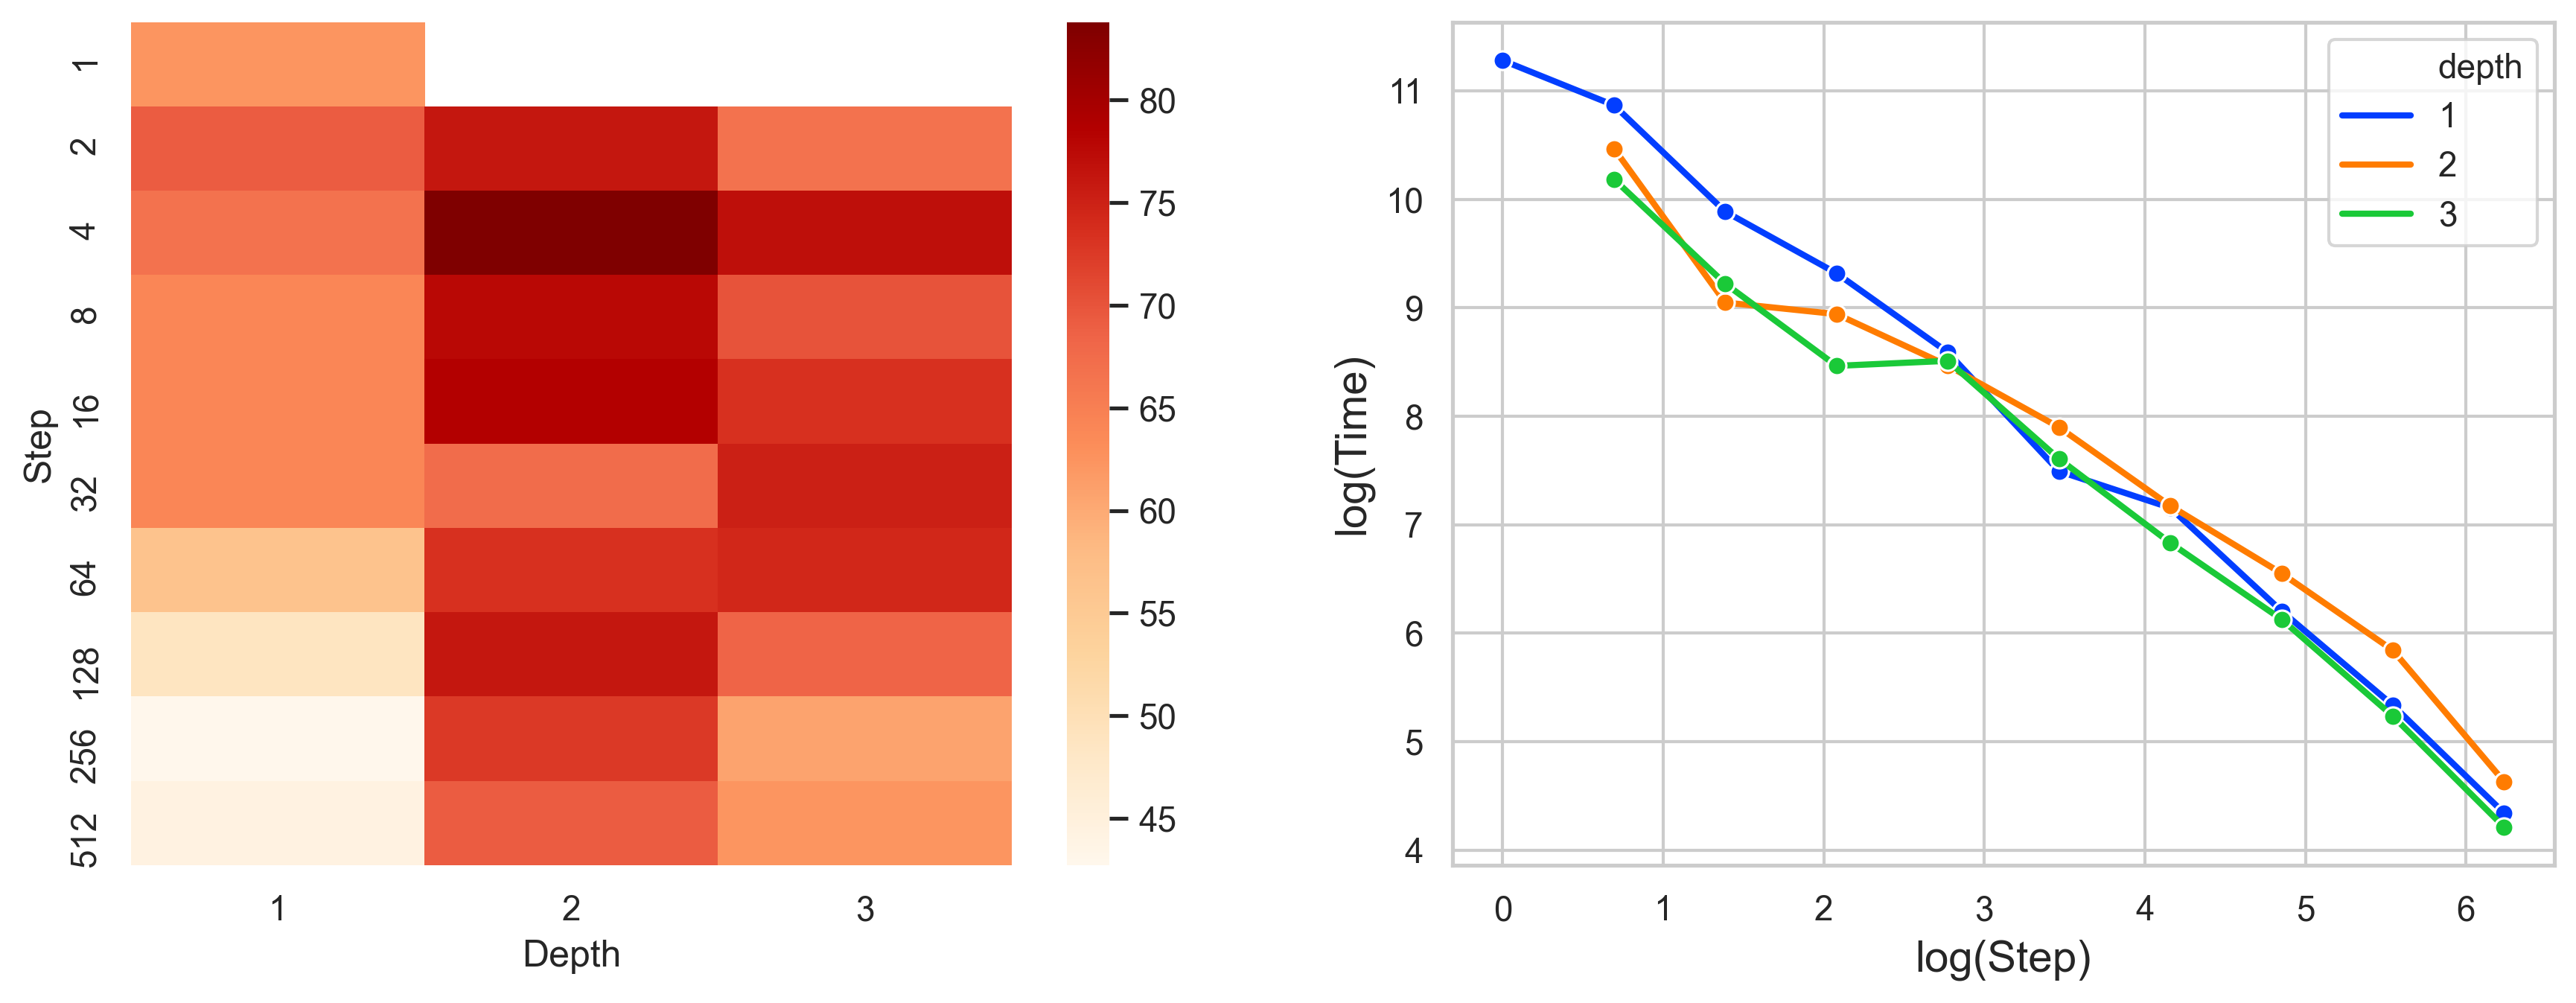
\includegraphics[width=0.95\textwidth]{Images/eigenworms.png}
    \caption{\textbf{Left:} Heatmap of accuracies on the EigenWorms dataset for differing step sizes and depths. \textbf{Right:} Log-log plot of the elapsed time of the algorithm against the step size.}
    \label{fig:eigenworms}
\end{figure}

\begin{table}[t]
    \begin{center}
        \begin{tabular}{ccccc}
        \toprule
        \textbf{Model} & \textbf{Step} & \textbf{Test Accuracy (\%)} & \textbf{Time (Hrs)} & \textbf{Memory (Mb)} \\
        \midrule
        & 1   &  62.4 $\pm$ 12.1 &          22.0 &         176.5 \\
        \multirow{2}{*}{NCDE$_1$}  & 8   &  64.1 $\pm$ 13.3 &           3.1 &          24.3 \\
        & 32  &  64.1 $\pm$ 14.3 &           0.5 &           8.0 \\
        & 128 &   48.7 $\pm$ 2.6 &           0.1 &           3.9 \\
        \midrule
        & 8   &   \textbf{77.8 $\pm$ 5.9} &           2.1 &          94.2 \\
        NCDE$_2$ & 32  &  67.5 $\pm$ 12.1 &           0.7 &          28.1 \\
          & 128 &   \textbf{76.1 $\pm$ 5.9} &           0.2 &           7.8 \\
        \hdashline\noalign{\vskip 0.5ex}
        & 8   &   70.1 $\pm$ 6.5 &           1.3 &         460.7 \\
        NCDE$_3$ & 32  &   \textbf{75.2 $\pm$ 3.0} &           0.6 &         134.7 \\
        & 128 &   68.4 $\pm$ 8.2 &           0.1 &          53.3 \\
        \bottomrule
        \end{tabular}
    \end{center}
    \caption{Performance on the UEA EigenWorms dataset for depths 1-3 and a selection of step sizes. Bold denotes that the model was the top performer for that step-size.}
    \label{tab:eigenworms}
\end{table}

See Table \ref{tab:eigenworms}. We see that the straightforward $\mathrm{NCDE}^1_1$ model takes roughly a day to train. Using the log-ODE method ($\mathrm{NCDE}_2$, $\mathrm{NCDE}_3$) speeds this up to take roughly minutes. Doing so additionally improves model performance dramatically, and reduces memory usage. Naive subsampling approaches ($\mathrm{NCDE}^{8}_1$, $\mathrm{NCDE}^{32}_1$, $\mathrm{NCDE}^{128}_1$) only achieve speedups without performance improvements.

See also Figure \ref{fig:eigenworms}, in which we summarise results for a larger range of step sizes.

\subsection{Estimating Vitals Signs from PPG and ECG Data}
Next we consider the problem of estimating vital signs from PPG and ECG data. The data is taken from the TSR archive \cite{MonashTSRegressionArchive} and involves data from the Beth Israel Deaconess Medical Centre (BIDMC). We consider three tasks whereby we aim to predict a persons respiratory rate (RR), their heart rate (HR), and their oxygen saturation (SpO2). This data is sampled at 125hZ with each series having a length of 4000, 7949 training samples, and a dimension of 3 (including time).

We train a model on each of the three vitals sign prediction tasks using a similar approach to the EigenWorms dataset. The metric used to evaluate performance is the root mean squared error (RMSE) loss which is the standard loss considered in the TSR archive. The results over a range of step sizes are presented in table (\ref{tab:bidmc}). The full results over all step sizes, along with a plots analogous to figure \ref{fig:eigenworms} are left to Appendix \ref{apx:results}.

\begin{table}[t]
    \small
    \begin{center}
        \begin{tabular}{ccccccccc}
        \toprule
        \multirow{2}{*}{\textbf{Depth}} & \multirow{2}{*}{\textbf{Step}} & \multicolumn{3}{c}{\textbf{RMSE}} & \multicolumn{3}{c}{\textbf{Time (H)}} & \multirow{2}{*}{\textbf{Memory (Mb)}} \\
        \cmidrule(lr){3-5} \cmidrule(lr){6-8}
         & & RR & HR & SpO$_2$ & RR & HR & SpO$_2$ & \\
         \midrule
        & 1   &  2.79 $\pm$ 0.04 &   9.82 $\pm$ 0.34 &  2.83 $\pm$ 0.27 &          23.8 &          22.1 &          28.1 &               56.5 \\
        \multirow{2}{*}{NCDE$_1$} & 8   &   2.80 $\pm$ 0.06 &  10.72 $\pm$ 0.24 &  3.43 $\pm$ 0.17 &           3.0 &           2.6 &           4.8 &               14.3 \\
          & 32  &  2.53 $\pm$ 0.23 &  12.23 $\pm$ 0.43 &  2.68 $\pm$ 0.12 &           1.9 &           0.9 &           2.2 &                9.8 \\
          & 128 &  2.64 $\pm$ 0.18 &  11.98 $\pm$ 0.37 &  2.86 $\pm$ 0.04 &           0.2 &           0.2 &           0.3 &                8.7 \\
        \midrule
        & 8   &  2.63 $\pm$ 0.12 &   8.63 $\pm$ 0.24 &  2.88 $\pm$ 0.15 &           2.1 &           3.4 &           3.3 &               21.8 \\
        NCDE$_2$ & 32  &   1.90 $\pm$ 0.02 &     7.90 $\pm$ 1.00 &   1.69 $\pm$ 0.20 &           1.2 &           1.1 &           2.0 &               13.1 \\
          & 128 &  1.86 $\pm$ 0.03 &   6.77 $\pm$ 0.42 &  1.95 $\pm$ 0.18 &           0.3 &           0.4 &           0.7 &               10.9 \\
        \hdashline\noalign{\vskip 0.5ex}
        & 8   &  \textbf{2.42 $\pm$ 0.19} &    \textbf{7.67 $\pm$ 0.40} &  \textbf{2.55 $\pm$ 0.13} &           2.9 &           3.2 &           3.1 &               43.3 \\
        NCDE$_3$ & 32  &  \textbf{1.67 $\pm$ 0.01} &    \textbf{4.50 $\pm$ 0.70} &  \textbf{1.61 $\pm$ 0.05} &           1.3 &           1.8 &           7.3 &               20.5 \\
          & 128 & \textbf{1.51 $\pm$ 0.08} &  \textbf{2.97 $\pm$ 0.45} &  \textbf{1.37 $\pm$ 0.22} &           0.5 &           1.7 &           1.7 &               17.3 \\
        \bottomrule
        \end{tabular}
    \end{center}
    \caption{The RMSE scores on the test set for each of the vitals signs prediction tasks (RR, HR, SpO$_2$) on the BIDMC dataset. The memory usage is given as the mean over all three of the tasks as it was approximately the same for any task for a given depth and step. The bold values denote the algorithm with the lowest test set loss for a fixed step size for each task.}
    \label{tab:bidmc}
\end{table}

We find that the depth $3$ model is the top performer for every task at any step size. Whats more, the top performing depth 3 model from each category also significantly outperforms the NCDE$^1_1$ model with a significantly reduced training time. This again illustrates that the increased step size not only reduces training time, but can also improve model performance. We believe this is attributable to the log-ODE model being better at learning these long-term dependencies, as the worst scores of the NCDE$^s_{2, 3}$ models are with step sizes 2 and 4 for all tasks where they are on par (or worse) than the corresponding depth 1 model.

Both experiments give show that the depth 2 and 3 models can not only reduce training times with similar levels of performance, but can additionally result in improved performance over these large steps. 


\section{Limitations}

\paragraph{Number of hyperparameters} Two new hyperparameters -- truncation depth and step size -- with substantial effects on training time and memory usage must now also be tuned.

\paragraph{Number of input channels} The log-ODE method is most feasible for low numbers of input channels, as the number of logsignature channels $\beta(v, N)$ grows near-exponentially in $v$.

\section{Related Work}
There has been some work on long time series for classic RNN (GRU/LSTM) models. \citet{campos2017skip} introduce the `Skip-RNN' model, which extend the RNN by adding an additional learnt component that skips state updates. This reduces the number of computations in the forward pass. However, this model is now not dependent on the within-skip input data. Furthermore, one does not know a priori how many states the model will choose to skip, which can lead to memory difficulties. 

Another approach is hierarchical subsampling as in \citet{graves2012supervised, de2015survey}, which operates over multiple training examples at a time as an input, thus reducing the number of total forward computations. Whilst this method is dependent on all the data, it naively uses the raw data when an appropriate summarisation would be more sensible.

This is rectified in \cite{liao2019learning} where the authors in fact use the logsignature as their summarisation procedure.


However, as is common with all of these models, it describes some some modification of the RNN structure but it has been shown in \cite{kidger2020neural} that the NCDE model subsumes the class of RNN/LSTM/GRU, in that it can model a wider class of functions. Additionally, none of these approaches be solved using ODE methods and thus are not able to utilise the adjoint method, continuous time dynamics, and so on.   


\section{Conclusions}
We have shown how the integral equation from the Neural CDE model can be solved with high accuracy over intervals larger than the discretisation of the data can be solved using the log-ODE method. We demonstrated that this not only enables us to take longer steps over the data whilst retaining model performance resulting in significantly lower training times, but also that this can result in models that achieve better performance over large step sizes than the original model over any step size, including updating the hidden state at every data point. 




\subsubsection*{Author Contributions}


\subsubsection*{Acknowledgements}
JM was supported by the EPSRC grant EP/L015803/1 in collaboration
with Iterex Therapuetics. CS was supported by the
EPSRC grant EP/R513295/1. PK was supported by the EPSRC grant EP/L015811/1. JF was supported by the EPSRC grant EP/N509711/1. JM, CS, PK, JF, TL were supported by the Alan Turing Institute under the EPSRC grant EP/N510129/1.


\bibliography{bibliography}
\bibliographystyle{style/iclr2020_conference}

\newpage

\documentclass{article} % For LaTeX2e
\usepackage{style/iclr2020_conference,times}

% Optional math commands from https://github.com/goodfeli/dlbook_notation.
%%%%% NEW MATH DEFINITIONS %%%%%

\usepackage{amsmath,amsfonts,bm}

% Mark sections of captions for referring to divisions of figures
\newcommand{\figleft}{{\em (Left)}}
\newcommand{\figcenter}{{\em (Center)}}
\newcommand{\figright}{{\em (Right)}}
\newcommand{\figtop}{{\em (Top)}}
\newcommand{\figbottom}{{\em (Bottom)}}
\newcommand{\captiona}{{\em (a)}}
\newcommand{\captionb}{{\em (b)}}
\newcommand{\captionc}{{\em (c)}}
\newcommand{\captiond}{{\em (d)}}

% Highlight a newly defined term
\newcommand{\newterm}[1]{{\bf #1}}


% Figure reference, lower-case.
\def\figref#1{figure~\ref{#1}}
% Figure reference, capital. For start of sentence
\def\Figref#1{Figure~\ref{#1}}
\def\twofigref#1#2{figures \ref{#1} and \ref{#2}}
\def\quadfigref#1#2#3#4{figures \ref{#1}, \ref{#2}, \ref{#3} and \ref{#4}}
% Section reference, lower-case.
\def\secref#1{section~\ref{#1}}
% Section reference, capital.
\def\Secref#1{Section~\ref{#1}}
% Reference to two sections.
\def\twosecrefs#1#2{sections \ref{#1} and \ref{#2}}
% Reference to three sections.
\def\secrefs#1#2#3{sections \ref{#1}, \ref{#2} and \ref{#3}}
% Reference to an equation, lower-case.
\def\eqref#1{equation~\ref{#1}}
% Reference to an equation, upper case
\def\Eqref#1{Equation~\ref{#1}}
% A raw reference to an equation---avoid using if possible
\def\plaineqref#1{\ref{#1}}
% Reference to a chapter, lower-case.
\def\chapref#1{chapter~\ref{#1}}
% Reference to an equation, upper case.
\def\Chapref#1{Chapter~\ref{#1}}
% Reference to a range of chapters
\def\rangechapref#1#2{chapters\ref{#1}--\ref{#2}}
% Reference to an algorithm, lower-case.
\def\algref#1{algorithm~\ref{#1}}
% Reference to an algorithm, upper case.
\def\Algref#1{Algorithm~\ref{#1}}
\def\twoalgref#1#2{algorithms \ref{#1} and \ref{#2}}
\def\Twoalgref#1#2{Algorithms \ref{#1} and \ref{#2}}
% Reference to a part, lower case
\def\partref#1{part~\ref{#1}}
% Reference to a part, upper case
\def\Partref#1{Part~\ref{#1}}
\def\twopartref#1#2{parts \ref{#1} and \ref{#2}}

\def\ceil#1{\lceil #1 \rceil}
\def\floor#1{\lfloor #1 \rfloor}
\def\1{\bm{1}}
\newcommand{\train}{\mathcal{D}}
\newcommand{\valid}{\mathcal{D_{\mathrm{valid}}}}
\newcommand{\test}{\mathcal{D_{\mathrm{test}}}}

\def\eps{{\epsilon}}


% Random variables
\def\reta{{\textnormal{$\eta$}}}
\def\ra{{\textnormal{a}}}
\def\rb{{\textnormal{b}}}
\def\rc{{\textnormal{c}}}
\def\rd{{\textnormal{d}}}
\def\re{{\textnormal{e}}}
\def\rf{{\textnormal{f}}}
\def\rg{{\textnormal{g}}}
\def\rh{{\textnormal{h}}}
\def\ri{{\textnormal{i}}}
\def\rj{{\textnormal{j}}}
\def\rk{{\textnormal{k}}}
\def\rl{{\textnormal{l}}}
% rm is already a command, just don't name any random variables m
\def\rn{{\textnormal{n}}}
\def\ro{{\textnormal{o}}}
\def\rp{{\textnormal{p}}}
\def\rq{{\textnormal{q}}}
\def\rr{{\textnormal{r}}}
\def\rs{{\textnormal{s}}}
\def\rt{{\textnormal{t}}}
\def\ru{{\textnormal{u}}}
\def\rv{{\textnormal{v}}}
\def\rw{{\textnormal{w}}}
\def\rx{{\textnormal{x}}}
\def\ry{{\textnormal{y}}}
\def\rz{{\textnormal{z}}}

% Random vectors
\def\rvepsilon{{\mathbf{\epsilon}}}
\def\rvtheta{{\mathbf{\theta}}}
\def\rva{{\mathbf{a}}}
\def\rvb{{\mathbf{b}}}
\def\rvc{{\mathbf{c}}}
\def\rvd{{\mathbf{d}}}
\def\rve{{\mathbf{e}}}
\def\rvf{{\mathbf{f}}}
\def\rvg{{\mathbf{g}}}
\def\rvh{{\mathbf{h}}}
\def\rvu{{\mathbf{i}}}
\def\rvj{{\mathbf{j}}}
\def\rvk{{\mathbf{k}}}
\def\rvl{{\mathbf{l}}}
\def\rvm{{\mathbf{m}}}
\def\rvn{{\mathbf{n}}}
\def\rvo{{\mathbf{o}}}
\def\rvp{{\mathbf{p}}}
\def\rvq{{\mathbf{q}}}
\def\rvr{{\mathbf{r}}}
\def\rvs{{\mathbf{s}}}
\def\rvt{{\mathbf{t}}}
\def\rvu{{\mathbf{u}}}
\def\rvv{{\mathbf{v}}}
\def\rvw{{\mathbf{w}}}
\def\rvx{{\mathbf{x}}}
\def\rvy{{\mathbf{y}}}
\def\rvz{{\mathbf{z}}}

% Elements of random vectors
\def\erva{{\textnormal{a}}}
\def\ervb{{\textnormal{b}}}
\def\ervc{{\textnormal{c}}}
\def\ervd{{\textnormal{d}}}
\def\erve{{\textnormal{e}}}
\def\ervf{{\textnormal{f}}}
\def\ervg{{\textnormal{g}}}
\def\ervh{{\textnormal{h}}}
\def\ervi{{\textnormal{i}}}
\def\ervj{{\textnormal{j}}}
\def\ervk{{\textnormal{k}}}
\def\ervl{{\textnormal{l}}}
\def\ervm{{\textnormal{m}}}
\def\ervn{{\textnormal{n}}}
\def\ervo{{\textnormal{o}}}
\def\ervp{{\textnormal{p}}}
\def\ervq{{\textnormal{q}}}
\def\ervr{{\textnormal{r}}}
\def\ervs{{\textnormal{s}}}
\def\ervt{{\textnormal{t}}}
\def\ervu{{\textnormal{u}}}
\def\ervv{{\textnormal{v}}}
\def\ervw{{\textnormal{w}}}
\def\ervx{{\textnormal{x}}}
\def\ervy{{\textnormal{y}}}
\def\ervz{{\textnormal{z}}}

% Random matrices
\def\rmA{{\mathbf{A}}}
\def\rmB{{\mathbf{B}}}
\def\rmC{{\mathbf{C}}}
\def\rmD{{\mathbf{D}}}
\def\rmE{{\mathbf{E}}}
\def\rmF{{\mathbf{F}}}
\def\rmG{{\mathbf{G}}}
\def\rmH{{\mathbf{H}}}
\def\rmI{{\mathbf{I}}}
\def\rmJ{{\mathbf{J}}}
\def\rmK{{\mathbf{K}}}
\def\rmL{{\mathbf{L}}}
\def\rmM{{\mathbf{M}}}
\def\rmN{{\mathbf{N}}}
\def\rmO{{\mathbf{O}}}
\def\rmP{{\mathbf{P}}}
\def\rmQ{{\mathbf{Q}}}
\def\rmR{{\mathbf{R}}}
\def\rmS{{\mathbf{S}}}
\def\rmT{{\mathbf{T}}}
\def\rmU{{\mathbf{U}}}
\def\rmV{{\mathbf{V}}}
\def\rmW{{\mathbf{W}}}
\def\rmX{{\mathbf{X}}}
\def\rmY{{\mathbf{Y}}}
\def\rmZ{{\mathbf{Z}}}

% Elements of random matrices
\def\ermA{{\textnormal{A}}}
\def\ermB{{\textnormal{B}}}
\def\ermC{{\textnormal{C}}}
\def\ermD{{\textnormal{D}}}
\def\ermE{{\textnormal{E}}}
\def\ermF{{\textnormal{F}}}
\def\ermG{{\textnormal{G}}}
\def\ermH{{\textnormal{H}}}
\def\ermI{{\textnormal{I}}}
\def\ermJ{{\textnormal{J}}}
\def\ermK{{\textnormal{K}}}
\def\ermL{{\textnormal{L}}}
\def\ermM{{\textnormal{M}}}
\def\ermN{{\textnormal{N}}}
\def\ermO{{\textnormal{O}}}
\def\ermP{{\textnormal{P}}}
\def\ermQ{{\textnormal{Q}}}
\def\ermR{{\textnormal{R}}}
\def\ermS{{\textnormal{S}}}
\def\ermT{{\textnormal{T}}}
\def\ermU{{\textnormal{U}}}
\def\ermV{{\textnormal{V}}}
\def\ermW{{\textnormal{W}}}
\def\ermX{{\textnormal{X}}}
\def\ermY{{\textnormal{Y}}}
\def\ermZ{{\textnormal{Z}}}

% Vectors
\def\vzero{{\bm{0}}}
\def\vone{{\bm{1}}}
\def\vmu{{\bm{\mu}}}
\def\vtheta{{\bm{\theta}}}
\def\va{{\bm{a}}}
\def\vb{{\bm{b}}}
\def\vc{{\bm{c}}}
\def\vd{{\bm{d}}}
\def\ve{{\bm{e}}}
\def\vf{{\bm{f}}}
\def\vg{{\bm{g}}}
\def\vh{{\bm{h}}}
\def\vi{{\bm{i}}}
\def\vj{{\bm{j}}}
\def\vk{{\bm{k}}}
\def\vl{{\bm{l}}}
\def\vm{{\bm{m}}}
\def\vn{{\bm{n}}}
\def\vo{{\bm{o}}}
\def\vp{{\bm{p}}}
\def\vq{{\bm{q}}}
\def\vr{{\bm{r}}}
\def\vs{{\bm{s}}}
\def\vt{{\bm{t}}}
\def\vu{{\bm{u}}}
\def\vv{{\bm{v}}}
\def\vw{{\bm{w}}}
\def\vx{{\bm{x}}}
\def\vy{{\bm{y}}}
\def\vz{{\bm{z}}}

% Elements of vectors
\def\evalpha{{\alpha}}
\def\evbeta{{\beta}}
\def\evepsilon{{\epsilon}}
\def\evlambda{{\lambda}}
\def\evomega{{\omega}}
\def\evmu{{\mu}}
\def\evpsi{{\psi}}
\def\evsigma{{\sigma}}
\def\evtheta{{\theta}}
\def\eva{{a}}
\def\evb{{b}}
\def\evc{{c}}
\def\evd{{d}}
\def\eve{{e}}
\def\evf{{f}}
\def\evg{{g}}
\def\evh{{h}}
\def\evi{{i}}
\def\evj{{j}}
\def\evk{{k}}
\def\evl{{l}}
\def\evm{{m}}
\def\evn{{n}}
\def\evo{{o}}
\def\evp{{p}}
\def\evq{{q}}
\def\evr{{r}}
\def\evs{{s}}
\def\evt{{t}}
\def\evu{{u}}
\def\evv{{v}}
\def\evw{{w}}
\def\evx{{x}}
\def\evy{{y}}
\def\evz{{z}}

% Matrix
\def\mA{{\bm{A}}}
\def\mB{{\bm{B}}}
\def\mC{{\bm{C}}}
\def\mD{{\bm{D}}}
\def\mE{{\bm{E}}}
\def\mF{{\bm{F}}}
\def\mG{{\bm{G}}}
\def\mH{{\bm{H}}}
\def\mI{{\bm{I}}}
\def\mJ{{\bm{J}}}
\def\mK{{\bm{K}}}
\def\mL{{\bm{L}}}
\def\mM{{\bm{M}}}
\def\mN{{\bm{N}}}
\def\mO{{\bm{O}}}
\def\mP{{\bm{P}}}
\def\mQ{{\bm{Q}}}
\def\mR{{\bm{R}}}
\def\mS{{\bm{S}}}
\def\mT{{\bm{T}}}
\def\mU{{\bm{U}}}
\def\mV{{\bm{V}}}
\def\mW{{\bm{W}}}
\def\mX{{\bm{X}}}
\def\mY{{\bm{Y}}}
\def\mZ{{\bm{Z}}}
\def\mBeta{{\bm{\beta}}}
\def\mPhi{{\bm{\Phi}}}
\def\mLambda{{\bm{\Lambda}}}
\def\mSigma{{\bm{\Sigma}}}

% Tensor
\DeclareMathAlphabet{\mathsfit}{\encodingdefault}{\sfdefault}{m}{sl}
\SetMathAlphabet{\mathsfit}{bold}{\encodingdefault}{\sfdefault}{bx}{n}
\newcommand{\tens}[1]{\bm{\mathsfit{#1}}}
\def\tA{{\tens{A}}}
\def\tB{{\tens{B}}}
\def\tC{{\tens{C}}}
\def\tD{{\tens{D}}}
\def\tE{{\tens{E}}}
\def\tF{{\tens{F}}}
\def\tG{{\tens{G}}}
\def\tH{{\tens{H}}}
\def\tI{{\tens{I}}}
\def\tJ{{\tens{J}}}
\def\tK{{\tens{K}}}
\def\tL{{\tens{L}}}
\def\tM{{\tens{M}}}
\def\tN{{\tens{N}}}
\def\tO{{\tens{O}}}
\def\tP{{\tens{P}}}
\def\tQ{{\tens{Q}}}
\def\tR{{\tens{R}}}
\def\tS{{\tens{S}}}
\def\tT{{\tens{T}}}
\def\tU{{\tens{U}}}
\def\tV{{\tens{V}}}
\def\tW{{\tens{W}}}
\def\tX{{\tens{X}}}
\def\tY{{\tens{Y}}}
\def\tZ{{\tens{Z}}}


% Graph
\def\gA{{\mathcal{A}}}
\def\gB{{\mathcal{B}}}
\def\gC{{\mathcal{C}}}
\def\gD{{\mathcal{D}}}
\def\gE{{\mathcal{E}}}
\def\gF{{\mathcal{F}}}
\def\gG{{\mathcal{G}}}
\def\gH{{\mathcal{H}}}
\def\gI{{\mathcal{I}}}
\def\gJ{{\mathcal{J}}}
\def\gK{{\mathcal{K}}}
\def\gL{{\mathcal{L}}}
\def\gM{{\mathcal{M}}}
\def\gN{{\mathcal{N}}}
\def\gO{{\mathcal{O}}}
\def\gP{{\mathcal{P}}}
\def\gQ{{\mathcal{Q}}}
\def\gR{{\mathcal{R}}}
\def\gS{{\mathcal{S}}}
\def\gT{{\mathcal{T}}}
\def\gU{{\mathcal{U}}}
\def\gV{{\mathcal{V}}}
\def\gW{{\mathcal{W}}}
\def\gX{{\mathcal{X}}}
\def\gY{{\mathcal{Y}}}
\def\gZ{{\mathcal{Z}}}

% Sets
\def\sA{{\mathbb{A}}}
\def\sB{{\mathbb{B}}}
\def\sC{{\mathbb{C}}}
\def\sD{{\mathbb{D}}}
% Don't use a set called E, because this would be the same as our symbol
% for expectation.
\def\sF{{\mathbb{F}}}
\def\sG{{\mathbb{G}}}
\def\sH{{\mathbb{H}}}
\def\sI{{\mathbb{I}}}
\def\sJ{{\mathbb{J}}}
\def\sK{{\mathbb{K}}}
\def\sL{{\mathbb{L}}}
\def\sM{{\mathbb{M}}}
\def\sN{{\mathbb{N}}}
\def\sO{{\mathbb{O}}}
\def\sP{{\mathbb{P}}}
\def\sQ{{\mathbb{Q}}}
\def\sR{{\mathbb{R}}}
\def\sS{{\mathbb{S}}}
\def\sT{{\mathbb{T}}}
\def\sU{{\mathbb{U}}}
\def\sV{{\mathbb{V}}}
\def\sW{{\mathbb{W}}}
\def\sX{{\mathbb{X}}}
\def\sY{{\mathbb{Y}}}
\def\sZ{{\mathbb{Z}}}

% Entries of a matrix
\def\emLambda{{\Lambda}}
\def\emA{{A}}
\def\emB{{B}}
\def\emC{{C}}
\def\emD{{D}}
\def\emE{{E}}
\def\emF{{F}}
\def\emG{{G}}
\def\emH{{H}}
\def\emI{{I}}
\def\emJ{{J}}
\def\emK{{K}}
\def\emL{{L}}
\def\emM{{M}}
\def\emN{{N}}
\def\emO{{O}}
\def\emP{{P}}
\def\emQ{{Q}}
\def\emR{{R}}
\def\emS{{S}}
\def\emT{{T}}
\def\emU{{U}}
\def\emV{{V}}
\def\emW{{W}}
\def\emX{{X}}
\def\emY{{Y}}
\def\emZ{{Z}}
\def\emSigma{{\Sigma}}

% entries of a tensor
% Same font as tensor, without \bm wrapper
\newcommand{\etens}[1]{\mathsfit{#1}}
\def\etLambda{{\etens{\Lambda}}}
\def\etA{{\etens{A}}}
\def\etB{{\etens{B}}}
\def\etC{{\etens{C}}}
\def\etD{{\etens{D}}}
\def\etE{{\etens{E}}}
\def\etF{{\etens{F}}}
\def\etG{{\etens{G}}}
\def\etH{{\etens{H}}}
\def\etI{{\etens{I}}}
\def\etJ{{\etens{J}}}
\def\etK{{\etens{K}}}
\def\etL{{\etens{L}}}
\def\etM{{\etens{M}}}
\def\etN{{\etens{N}}}
\def\etO{{\etens{O}}}
\def\etP{{\etens{P}}}
\def\etQ{{\etens{Q}}}
\def\etR{{\etens{R}}}
\def\etS{{\etens{S}}}
\def\etT{{\etens{T}}}
\def\etU{{\etens{U}}}
\def\etV{{\etens{V}}}
\def\etW{{\etens{W}}}
\def\etX{{\etens{X}}}
\def\etY{{\etens{Y}}}
\def\etZ{{\etens{Z}}}

% The true underlying data generating distribution
\newcommand{\pdata}{p_{\rm{data}}}
% The empirical distribution defined by the training set
\newcommand{\ptrain}{\hat{p}_{\rm{data}}}
\newcommand{\Ptrain}{\hat{P}_{\rm{data}}}
% The model distribution
\newcommand{\pmodel}{p_{\rm{model}}}
\newcommand{\Pmodel}{P_{\rm{model}}}
\newcommand{\ptildemodel}{\tilde{p}_{\rm{model}}}
% Stochastic autoencoder distributions
\newcommand{\pencode}{p_{\rm{encoder}}}
\newcommand{\pdecode}{p_{\rm{decoder}}}
\newcommand{\precons}{p_{\rm{reconstruct}}}

\newcommand{\laplace}{\mathrm{Laplace}} % Laplace distribution

\newcommand{\E}{\mathbb{E}}
\newcommand{\Ls}{\mathcal{L}}
\newcommand{\R}{\mathbb{R}}
\newcommand{\emp}{\tilde{p}}
\newcommand{\lr}{\alpha}
\newcommand{\reg}{\lambda}
\newcommand{\rect}{\mathrm{rectifier}}
\newcommand{\softmax}{\mathrm{softmax}}
\newcommand{\sigmoid}{\sigma}
\newcommand{\softplus}{\zeta}
\newcommand{\KL}{D_{\mathrm{KL}}}
\newcommand{\Var}{\mathrm{Var}}
\newcommand{\standarderror}{\mathrm{SE}}
\newcommand{\Cov}{\mathrm{Cov}}
\newcommand{\m}{\hspace{0.25mm}}
\newcommand{\mm}{\hspace{5mm}}
\newcommand{\D}{\mathcal{D}}
% Wolfram Mathworld says $L^2$ is for function spaces and $\ell^2$ is for vectors
% But then they seem to use $L^2$ for vectors throughout the site, and so does
% wikipedia.
\newcommand{\normlzero}{L^0}
\newcommand{\normlone}{L^1}
\newcommand{\normltwo}{L^2}
\newcommand{\normlp}{L^p}
\newcommand{\normmax}{L^\infty}
\newcommand{\parents}{Pa} % See usage in notation.tex. Chosen to match Daphne's book.

\DeclareMathOperator*{\argmax}{arg\,max}
\DeclareMathOperator*{\argmin}{arg\,min}

\DeclareMathOperator{\sign}{sign}
\DeclareMathOperator{\Tr}{Tr}
\let\ab\allowbreak


\usepackage{hyperref}
\usepackage{url}

\usepackage{booktabs}       % professional-quality tables
\usepackage{arydshln}
\usepackage{amssymb}
\setlength\dashlinegap{2.5pt}

\usepackage{graphicx}
\usepackage{subcaption}
\usepackage{rotating}
\usepackage{ifthen}
\graphicspath{ {Images/} }

\newtheorem{theorem}{Theorem}[section]
\newtheorem{lemma}[theorem]{Lemma}
\newtheorem{prop}[theorem]{Proposition}
\newtheorem{proof}[theorem]{Proof}
\newtheorem{corollary}[theorem]{Corollary}
\newtheorem{method}[theorem]{Method}
\newtheorem{definition}[theorem]{Definition}
\newtheorem{example}[theorem]{Example}
\newtheorem{xca}[theorem]{Exercise}
\newtheorem{remark}[theorem]{Remark}

% This file contains lots of tikz stuff
% Tikz
\usepackage{ifthen}
\usepackage{intcalc}
\usepackage{tikz}
\usepackage{multirow}
\usetikzlibrary{decorations.pathreplacing,calligraphy}
\usetikzlibrary{arrows.meta, decorations.text, decorations.markings, decorations.pathreplacing, angles, quotes, calligraphy}
\definecolor{bittersweet}{rgb}{1.0, 0.44, 0.37}

% Logisig definitions
% Log-sig heights
\pgfmathsetmacro{\pathyshift}{0.8}
\global\def\rs{{0, 1, 2.1, 3.3, 4.5, 5.5, 6.5}}
\global\def\lsone{{2.15, 2.3, 2.1, 2.4, 2.1, 2.4}}
\global\def\lstwo{{2.1, 2.4, 2.2, 2.5, 2.2, 2.1}}
\global\def\lsthree{{2.3, 2.1, 2.15, 2.35, 2.5, 2.2}}
\global\def\lspathraise{0.7}
\global\def\data{{0.4, 0.7, 0.9, 0.5, 0.6, 0.9, 0.8, 0.5, 0.3, 0.3, 0.8, 1.0, 0.2, 0.4, 0.7, 0.5, 1.0, 1.0, 0.8, 0.4, 0.2, 0.6, 0.8, 0.5, 0.3, 0.5, 0.2, 0.1, 0.5, 0.2, 0.4, 0.6, 0.3, 0.2, 0.1, 0.7, 0.6, 0.2, 0.5, 0.4, 0.4, 0.1}}

% Logsig
\definecolor{colorls1}{HTML}{66C2A5}
\definecolor{colorls2}{HTML}{8DA0CB}
\definecolor{colorls3}{HTML}{FC8D62}

\newcommand\ncdediagram[1]{
    \begin{tikzpicture}
        % Choose between the logsig and normal version
        \pgfmathsetmacro{\logsigversion}{#1}
        
        % For reducing the height of the hidden state and integration steps in the two cases
        \ifthenelse{\logsigversion=0}
            {\pgfmathsetmacro{\hreduce}{1.8}}
            {\pgfmathsetmacro{\hreduce}{0}}
        
        % Time
        \draw[black, thick, ->] (0, 0) -- (7, 0);
        
        \ifthenelse{\logsigversion=0}
            {
                \foreach \i in {0, 6} {
                    \node at (\rs[\i], 0)[circle,fill, inner sep=1.5pt] {};
                }
                \node at (\rs[0], -0.25) {\tiny $t_0$};
                \node at (\rs[6], -0.25) {\tiny $t_m$};
            }
            {
                \foreach \i in {0, 1, 2, 3, 4, 5, 6} {
                    \node at (\rs[\i], 0)[circle,fill, inner sep=1.5pt] {};
                }
                \node at (\rs[0], -0.25) {\tiny $r_0$};
                \node at (\rs[1], -0.25) {\tiny $r_1$};
                \node at (\rs[2], -0.25) {\tiny $r_2$};
                \node at (\rs[3], -0.25) {\tiny $r_3$};
                \node at (\rs[4], -0.25) {\tiny $r_{m-2}$};
                \node at (\rs[5], -0.25) {\tiny $r_{m-1}$};
                \node at (\rs[6], -0.25) {\tiny $r_m$};
            }
        \node at (3.85, -0.25) {\tiny $\cdots$};
    
        
    
        
        \pgfmathsetmacro{\dataix}{0}
        \pgfmathsetmacro{\midwayprev}{0}
        \pgfmathsetmacro{\xprev}{0}
        \pgfmathsetmacro{\yprev}{0}
        \foreach \i in {0, 1, 2, 3, 4, 5} {
            % Macros
            \pgfmathsetmacro{\frac}{\rs[\i + 1] - \rs[\i]}
            \pgfmathsetmacro{\midway}{\rs[\i] + (\rs[\i + 1] - \rs[\i]) * 0.5}
            
            % Data and path
            \foreach \d in {0, 1, 2, 3, 4, 5, 6} {
                \ifthenelse{\i>0 \AND \d=0}{\pgfmathsetmacro{\y}{\data[\dataix - 1] * 0.5 + 0.1}}{\pgfmathsetmacro{\y}{\data[\dataix] * 0.5 + 0.1}}
                \pgfmathsetmacro{\x}{\rs[\i] + \d * \frac * 0.1667}
                \pgfmathsetmacro{\dx}{\frac * 0.1667}
                \ifthenelse{\i=3}
                    {
                        % Data
                        \node at (\x, \y)[circle, draw=black, fill=green!50, inner sep=1.5pt, opacity=0.3] {};
                        % Path
                        \node at (\x, \y + \pathyshift)[circle, draw=black, fill=green!50, inner sep=0.5pt, densely dashed] {};
                        \draw[green!50, thick, cap=round, dashed] (\xprev, \yprev + \pathyshift) -- (\x, \y + \pathyshift);
                    }
                    {
                        % Time tick
                        \ifthenelse{\logsigversion=0}{\draw (\x, -0.05) -- (\x, 0.05);}{}
                        % Data
                        \node at (\x, \y)[circle, draw=black, fill=green!50, inner sep=1.5pt] {};
                        % Path
                        \node at (\x, \y + \pathyshift)[circle, draw=black, fill=green!50, inner sep=0.5pt] {};
                        \ifthenelse{\i=0 \AND \d=0}{}{\draw[green!50, thick, cap=round] (\xprev, \yprev + \pathyshift) -- (\x, \y + \pathyshift);}
                        % Integration steps
                        \ifthenelse{\logsigversion=0}
                            {
                                \ifthenelse{\d=6 \AND \i=5}
                                    {}
                                    {
                                        \node at (\x, 3.8 - \hreduce)[circle, draw=black, fill=orange!50, inner sep=1.5pt] {};
                                    }
                            }
                            {}
                    }
                % Update globals
                \pgfmathsetmacro{\dataixnew}{\dataix + 1}
                \global\let\dataix=\dataixnew
                \global\let\yprev=\y
                \global\let\xprev=\x
                
            }
            
            \ifthenelse{\logsigversion=1}{
                \ifthenelse{\i=3}
                    {
                        % Integration steps
                        \node at (\rs[\i], 3.8)[circle, draw=black, fill=orange!50, inner sep=1.5pt] {};
                        \draw[->, dashed] (\rs[\i] + 0.08, 3.8) -- (\rs[\i+1] - 0.08, 3.8);
                        % % Brace
                        % \draw[decoration={calligraphic brace, amplitude=3pt}, decorate, line width=1pt, dotted] (\rs[\i] + 0.05, 1.65) node {} -- (\rs[\i+1] - 0.05, 1.65);
                        % % Brace arrow
                        % \draw[->, dashed] (\midway, 1.8) -- (\midway, 2.0);
                        % % Log-signatures
                        % \node at (\midway, \lsone[\i])[circle, draw=black, fill=colorls1, inner sep=1pt, opacity=0.3] {};
                        % \node at (\midway, \lstwo[\i])[circle, draw=black, fill=colorls2, inner sep=1pt, opacity=0.3] {};
                        % \node at (\midway, \lsthree[\i])[circle, draw=black, fill=colorls3, inner sep=1pt, opacity=0.3] {};
                    }
                    {
                        % Brace
                        \draw[decoration={calligraphic brace, amplitude=3pt}, decorate, line width=1pt] (\rs[\i] + 0.05, 1.65) node {} -- (\rs[\i+1] - 0.05, 1.65);
                        % Brace arrow
                        \draw[->, dashed] (\midway, 1.8) -- (\midway, 2.0);
                        % Log-signatures
                        \node at (\midway, \lsone[\i])[circle, draw=black, fill=colorls1, inner sep=1pt] {};
                        \node at (\midway, \lstwo[\i])[circle, draw=black, fill=colorls2, inner sep=1pt] {};
                        \node at (\midway, \lsthree[\i])[circle, draw=black, fill=colorls3, inner sep=1pt] {};
                        % Integration steps
                        \node at (\rs[\i], 3.8)[circle, draw=black, fill=orange!50, inner sep=1.5pt] {};
                        \draw[->] (\rs[\i] + 0.08, 3.8) -- (\rs[\i+1] - 0.08, 3.8);
                    }
                % Path raise
                \ifthenelse{\i=3}
                    {
                        
                    }
                    {
                        \node at (\midway, \lsone[\i] + \lspathraise)[circle, draw=black, fill=colorls1, inner sep=.5pt] {};
                        \node at (\midway, \lstwo[\i] + \lspathraise)[circle, draw=black, fill=colorls2, inner sep=.5pt] {};
                        \node at (\midway, \lsthree[\i] + \lspathraise)[circle, draw=black, fill=colorls3, inner sep=.5pt] {};
                    }
                % Log-sig path
                \ifthenelse{\i>0}
                    {   
                        % Horrendous code to dash out the middle logsig bit
                        \ifthenelse{\i=3 \OR \i=4}
                        {  
                            \ifthenelse{\i=3}
                                {
                                    \pgfmathsetmacro{\midmidway}{\midwayprev + (\midway - \midwayprev) * 0.5}
                                    \draw[colorls1, thick, cap=round] (\midwayprev, \lsone[\i-1] + \lspathraise) -- (\midmidway, \lsone[\i-1]*0.5 + \lsone[\i]*0.5 + \lspathraise);
                                    \draw[colorls1, thick, cap=round, densely dashed] (\midmidway, \lsone[\i-1]*0.5 + \lsone[\i]*0.5 + \lspathraise) -- (\midway, \lsone[\i] + \lspathraise);
                                    \draw[colorls2, thick, cap=round] (\midwayprev, \lstwo[\i-1] + \lspathraise) -- (\midmidway, \lstwo[\i-1]*0.5 + \lstwo[\i]*0.5 + \lspathraise);
                                    \draw[colorls2, thick, cap=round, densely dashed] (\midmidway, \lstwo[\i-1]*0.5 + \lstwo[\i]*0.5 + \lspathraise) -- (\midway, \lstwo[\i] + \lspathraise);
                                    \draw[colorls3, thick, cap=round] (\midwayprev, \lsthree[\i-1] + \lspathraise) -- (\midmidway, \lsthree[\i-1]*0.5 + \lsthree[\i]*0.5 + \lspathraise);
                                    \draw[colorls3, thick, cap=round, densely dashed] (\midmidway, \lsthree[\i-1]*0.5 + \lsthree[\i]*0.5 + \lspathraise) -- (\midway, \lsthree[\i] + \lspathraise);
                                }
                                {
                                    \pgfmathsetmacro{\midmidway}{\midwayprev + (\midway - \midwayprev) * 0.5}
                                    \draw[colorls1, thick, cap=round, densely dashed] (\midwayprev, \lsone[\i-1] + \lspathraise) -- (\midmidway, \lsone[\i-1]*0.5 + \lsone[\i]*0.5 + \lspathraise);
                                    \draw[colorls1, thick, cap=round] (\midmidway, \lsone[\i-1]*0.5 + \lsone[\i]*0.5 + \lspathraise) -- (\midway, \lsone[\i] + \lspathraise);
                                    \draw[colorls2, thick, cap=round, densely dashed] (\midwayprev, \lstwo[\i-1] + \lspathraise) -- (\midmidway, \lstwo[\i-1]*0.5 + \lstwo[\i]*0.5 + \lspathraise);
                                    \draw[colorls2, thick, cap=round] (\midmidway, \lstwo[\i-1]*0.5 + \lstwo[\i]*0.5 + \lspathraise) -- (\midway, \lstwo[\i] + \lspathraise);
                                    \draw[colorls3, thick, cap=round, densely dashed] (\midwayprev, \lsthree[\i-1] + \lspathraise) -- (\midmidway, \lsthree[\i-1]*0.5 + \lsthree[\i]*0.5 + \lspathraise);
                                    \draw[colorls3, thick, cap=round] (\midmidway, \lsthree[\i-1]*0.5 + \lsthree[\i]*0.5 + \lspathraise) -- (\midway, \lsthree[\i] + \lspathraise);
                                }
                        }
                        {
                            \draw[colorls1, thick, cap=round] (\midwayprev, \lsone[\i-1] + \lspathraise) -- (\midway, \lsone[\i] + \lspathraise);
                            \draw[colorls2, thick, cap=round] (\midwayprev, \lstwo[\i-1] + \lspathraise) -- (\midway, \lstwo[\i] + \lspathraise);
                            \draw[colorls3, thick, cap=round] (\midwayprev, \lsthree[\i-1] + \lspathraise) -- (\midway, \lsthree[\i] + \lspathraise);
                        }
                    }
                    {
                        \draw[colorls1, thick, cap=round] (\midwayprev, \lsone[\i] + \lspathraise) -- (\midway, \lsone[\i] + \lspathraise);
                        \draw[colorls2, thick, cap=round] (\midwayprev, \lstwo[\i] + \lspathraise) -- (\midway, \lstwo[\i] + \lspathraise);
                        \draw[colorls3, thick, cap=round] (\midwayprev, \lsthree[\i] + \lspathraise) -- (\midway, \lsthree[\i] + \lspathraise);
                    }
                \ifthenelse{\i=5} 
                    {
                        \draw[colorls1, thick, cap=round] (\midway, \lsone[\i] + \lspathraise) -- (\rs[\i+1], \lsone[\i] + \lspathraise);
                        \draw[colorls2, thick, cap=round] (\midway, \lstwo[\i] + \lspathraise) -- (\rs[\i+1], \lstwo[\i] + \lspathraise);
                        \draw[colorls3, thick, cap=round] (\midway, \lsthree[\i] + \lspathraise) -- (\rs[\i+1], \lsthree[\i] + \lspathraise);
                    }
                    {}
                }
                {
                }
                
            % Update globals
            \global\let\midwayprev=\midway
        }
        
        % Integration step arrow for non logsig
        \ifthenelse{\logsigversion=1}{}{\draw[->, dashed] (\rs[3] + 0.08, 3.8 - \hreduce) -- (\rs[4] - 0.08, 3.8 - \hreduce);}
        
        % Hidden state
        \draw[blue!50, thick, cap=round] (\rs[0], 4.8 - \hreduce) .. controls (0.5, 3.5 - \hreduce) and (2, 5.3 - \hreduce) .. (\rs[3], 4.8 - \hreduce);
        \draw[blue!50, thick, cap=round, dashed] (\rs[3], 4.8 - \hreduce) .. controls (\rs[3] + 0.2, 4.7 - \hreduce) and (\rs[4] - 0.2, 4.3 - \hreduce) .. (\rs[4], 4.3 - \hreduce);
        \draw[blue!50, thick, cap=round] (\rs[4], 4.3 - \hreduce) .. controls (\rs[4] + 0.3, 4.2 - \hreduce) and (\rs[6] - 0.4, 4.4 - \hreduce) .. (\rs[6], 4.7 - \hreduce);
    
        % Middle dots
        \ifthenelse{\logsigversion=1}
            {\node at (4, 1.7) {$\cdots$};}
            {}
        
        % RHS naming
        \node at (8, 0) {\footnotesize Time};
        \node (data) at (8, 0.4) {\footnotesize Data $\mathbf{x}$};
        \node (path) at (8, 1.15) {\footnotesize Path $X$};
        \ifthenelse{\logsigversion=1}{
            \node (logsig) at (8, 2.1) {\footnotesize $\mathrm{LogSig}_{r_i, r_{i+1}}(X)$}; 
            \node (logsig_path) at (8, 2.95) {\footnotesize Logsignature path}; 
        }{}
        \node (hidden) at (8, 4.7 - \hreduce) {\footnotesize Hidden state $Z_t$}; 
    
        % Arrows
        \draw[->] (data) -- (path);
        \ifthenelse{\logsigversion=1}
            {
                \draw[->] (path) -- (logsig);
                \draw[->] (logsig) -- (logsig_path);
                \draw [decorate, decoration={calligraphic brace,amplitude=1.5pt, mirror}] (6.5,3.6) -- node[midway, right, xshift=-5.5pt] {\scriptsize \begin{tabular}{l}Integration\\steps\end{tabular}} (6.5,4 - \hreduce);
                \draw[->] (logsig_path) -- (hidden);
            }
            {
                \draw [decorate, decoration={calligraphic brace,amplitude=1.5pt, mirror}] (6.5, 3.6 - \hreduce) -- node[midway, right, xshift=-5.5pt] {\scriptsize \begin{tabular}{l}Integration\\steps\end{tabular}} (6.5, 4 - \hreduce);
                \draw[->] (path) -- (hidden);
            }

    \end{tikzpicture}
}
\usetikzlibrary{external}

% Tikz network diagram
\tikzset{middlearrow/.style={
        decoration={markings,
            mark= at position 0.5 with {\arrow{#1}} ,
        },
        postaction={decorate}
    }
}
\tikzset{input/.style={black, draw=green!50, fill=green!50, rectangle, minimum height=0.8cm}}
\tikzset{hidden/.style={black, draw=blue!50, fill=blue!50, rectangle, minimum height=0.8cm}}
\tikzset{hidden_square/.style={black, draw=blue!50, fill=blue!50, rectangle, minimum height=3.5cm}}
\tikzset{logsig/.style={black, draw=red!50, fill=red!50, rectangle, minimum height=0.8cm}}


\title{Neural CDEs for Long Time Series via the Log-ODE Method}

% Authors must not appear in the submitted version. They should be hidden
% as long as the \iclrfinalcopy macro remains commented out below.
% Non-anonymous submissions will be rejected without review.

%\iclrfinalcopy

\author{James Morrill \And Patrick Kidger \And Cristopher Salvi  \And James Foster \And Terry Lyons\AND\\[-20pt]
Mathematical Institute, University of Oxford;\\
The Alan Turing Institute, British Library\\[2pt]
\texttt{\{morrill, kidger, salvi, foster, tlyons\}@maths.ox.ac.uk}
}

% The \author macro works with any number of authors. There are two commands
% used to separate the names and addresses of multiple authors: \And and \AND.
%
% Using \And between authors leaves it to \LaTeX{} to determine where to break
% the lines. Using \AND forces a linebreak at that point. So, if \LaTeX{}
% puts 3 of 4 authors names on the first line, and the last on the second
% line, try using \AND instead of \And before the third author name.

\newcommand{\fix}{\marginpar{FIX}}
\newcommand{\new}{\marginpar{NEW}}
\newcommand{\logsig}{\mathrm{LogSig}}
\newcommand{\dby}{\mathrm{d}}
\newcommand{\reals}{\mathbb{R}}
\newcommand{\naturals}{\mathbb{N}}
\newcommand{\restr}[2]{{\left.\kern-\nulldelimiterspace #1 \right|_{#2}}}

\begin{document}


\maketitle

\begin{abstract}
Neural Controlled Differential Equations (Neural CDEs) are the continuous-time analogue of an RNN, just as Neural ODEs are analogous to ResNets. However just like RNNs, training Neural CDEs is difficult for long time series. Training takes impractically long, and models may fail to train. Here, we demonstrate that an existing numerical method for the solution of CDEs -- the log-ODE method -- may in the context of Neural CDEs be used to take integration steps \emph{larger} than the discretisation of the data, whilst depending upon sub-step data through additional terms. Doing so represents making a length/channel trade-off, and is easy to implement with existing tools. We demonstrate efficacy on problems of length up to 17k observations and observe training speed-ups from roughly days to roughly minutes.
\end{abstract}


\section{Introduction}
Neural controlled differential equations (Neural CDEs) \citep{kidger2020neural} are the continuous-time analogue to a recurrent neural network (RNN), and provide a natural method for modelling temporal dynamics with neural networks.

Neural CDEs are similar to neural ordinary differential equations (Neural ODEs), as popularised by \citet{neural2018ode}. A Neural ODE is determined by its initial condition, without a direct way to modify the trajectory given subsequent observations. In contrast the vector field of a Neural CDE depends upon the time-varying data, so that changes in the data provoke in the local dynamics of the system.

\subsection{Controlled Differential Equations}
We begin by recalling the definition of a CDE.

Let $a, b \in \mathbb{R}$ with $a < b$, and let $v, w \in \mathbb{N}$. Let $\xi \in \mathbb{R}^w$. Let $X \colon [a, b] \to \mathbb{R}^v$ be a continuous function of bounded variation (which is for example implied by it being Lipschitz), and let $f~\colon~\mathbb{R}^w~\to~\mathbb{R}^{w \times v}$ be continuous.

Then we may define $Z: [a, b] \to \mathbb{R}^w$ as the unique solution of the \emph{controlled differential equation}
\begin{equation}
    Z_a = \xi,\qquad Z_t = Z_a + \int^{t}_{a} f(Z_s) \dby X_s \quad \text{for } t \in (a, b],
    \label{eq:kidger_cde}
\end{equation}
where the integral is a Riemann-Stieltjes integral. The notation ``$f(Z_s) \dby X_s$'' denotes a matrix-vector product, and if $X$ is differentiable then $\int_a^t f(Z_s) \dby X_s = \int_a^t f(Z_s) \frac{\dby X}{\dby s}(s) \dby s$.
% Add something about universality

If in equation (\ref{eq:kidger_cde}), $\dby X_s$ was replaced with $\dby s$, then the equation would just be an ODE. Using $\dby X_s$ causes the solution to depend continuously on changes in $X$.

\subsection{Neural Controlled Differential Equations}
We recall the definition of a Neural CDE as in \citet{kidger2020neural}.

Define a time series $\mathbf{x}$ as a collection of points $x_i \in \mathbb{R}^{v-1}$ with corresponding time-stamps $t_i \in \mathbb{R}$ such that $\mathbf{x} = ((t_0, x_0), (t_1, x_1), ..., (t_n, x_n))$, and $t_0 < ... < t_n$.

Let $X \colon [t_0, t_n] \to \reals^{v}$ be some interpolation of the data such that $X_{t_i} = (t_i, x_i)$. \citet{kidger2020neural} use natural cubic splines. Here we will actually end up finding piecewise linear interpolation to be a more convenient choice. (We avoid issues with adaptive solvers as discussed in \citet[Appendix A]{kidger2020neural} simply by using fixed solvers.) % TODO: discuss the linear interpolation paper once it's out.

Let $\xi_\theta \colon \reals^{v} \to \reals^w$ and $f_\theta \colon \reals^w \to \reals^{w \times v}$ be neural networks. Let $\ell_\theta \colon \reals^w \to \reals^{q}$ be linear, for some output dimension $q \in \naturals$. Here $\theta$ is used to denote dependence on learnable parameters.

We define $Z$ as the hidden state and $Y$ as the output of a \textit{neural controlled differential equation} driven by $X$ if
\begin{equation}
    Z_{t_0} = \xi_\theta(t_0, x_0), \quad \text{with} \quad  Z_t = Z_{t_0} + \int^{t}_{t_0} f_\theta(Z_s) \dby X_s \quad \text{and} \quad Y_t = \ell_\theta(Z_t) \quad \text{for } t \in (t_0, t_n].
    \label{eq:kidger_ncde}
\end{equation}

That is -- just like an RNN - we have evolving hidden state $Z$, which we take a linear map from to produce an output. This formulation is a universal approximator \citep[Appendix B]{kidger2020neural}. The output may be either the time-evolving $Y_t$ or just the final $Y_{t_n}$. This is then fed into a loss function ($L^2$, cross entropy, \ldots) and trained via stochastic gradient descent in the usual way.

The question remains how to compute the integral of equation (\ref{eq:kidger_ncde}). \citet{kidger2020neural} let
\begin{equation}
    g_{\theta, X}(Z, s) = f_\theta(Z) \frac{\dby X}{\dby s}(s),
    \label{eq:kidger_g_X}
\end{equation}
where the right hand side denotes a matrix multiplication, and then note that the integral can be written as
\begin{equation}
     Z_t = Z_{t_0} + \int^{t}_{t_0} g_{\theta, X}(Z_s, s) \dby s.
     \label{eq:kidger_cde_evaluation}
\end{equation}
This reduces the CDE to an ODE, so that existing tools for Neural ODEs may be used to evaluate this, and to backpropagate.

% To alleviate this, we can simply update the hidden state less frequently by skipping some of the time steps in the series. That is, we instead consider times $r_1,...,r_m$ where $r_m = t_n$, $r_i \geq t_i \; \forall i$ with typically $m << n$, and update with
% \begin{equation}
%      Z_{r_{i+1}} = Z_{r_i} + \int^{r_{i+1}}_{r_i} g_{\theta, X}(Z, s) \dby s.
%      \label{eq:kidger_cde_multi_data_update}
% \end{equation}
% Whilst this solves the training time time issue, it also results in a loss of information over each step as it utilises only information about the pointwise derivative at a fixed number of points.

\subsection{Applications}
By moving from the discrete-time formulation of an RNN to the continuous-time formulation of a Neural CDE, then all kinds of time series data are put on the same footing, whether it is regular or irregularly sampled, and whether or not it has missing values. The interpolation procedure for $X$ works regardless. Informative missingness is not sacrificed and can be incorporated by appending extra channels as usual.

Besides this, the continuous-time or differential equation formulation may be useful in applications where such models are explicitly desired, as when modelling physics.

% TODO: Add the NSDE paper once it's out.

\subsection{Contributions}
Neural CDEs, as with RNNs, begin to break down for long time series. Training loss/accuracy worsens, and training time becomes prohibitive due to the sheer number of forward operations within each training epoch.

Here, we propose to use the ``log-ODE method'', which is a numerical method for the solution of CDEs. In the CDE literature this is used as a way to handle roughness in $X$. Here, however, it instead becomes a principled way to trade length for channels. Loosely speaking, long time series are reduced to higher-dimensional short time series, and the problems attendant with length are alleviated. Training times may be improved from roughly days to roughly minutes, model performance is improved, and memory requirements are reduced.

The resulting scheme has two very neat interpretations. In terms of numerical differential equation solvers, this corresponds to taking integration steps larger than the discretisation the data, whilst incorporating sub-step information through additional terms.\footnote{For the reader familiar with numerical methods for SDEs, this is akin to the additional correction term in Milstein's method as compared to Euler--Maruyama.} In terms of machine learning, this corresponds to binning the data prior to running a Neural CDE, with bin statistics carefully chosen to extract precisely the information most relevant to solving a CDE. The method may be implemented as a relatively straightforward data preprocessing step.

% When evaluating equation (\ref{eq:kidger_cde_multi_data_update}) using the definition of $g_{\theta, X}$ as in equation (\ref{eq:kidger_g_X}), information about the structure of the data is only observed through the point-wise derivative of the interpolated data at a fixed number of points. The log-ODE method replaces the derivative function with something called the \textit{log-signature} of the path which provides essentially a compression of the data that holds more information than simply the derivative. We will show that in equation (\ref{eq:kidger_cde_multi_data_update}) we will instead  use
% \begin{equation}
%     g_{\theta, X}(Z, s) = f_\theta(Z) \logsig^N_{r_i, r_{i+1}}(X_s),
%     \label{eq:log-ode_update_simple}
% \end{equation}
% where this $\logsig^N_{r_i, r_{i+1}}(X_s)$ term is what provides us with additional information about the structure of the data over the interval resulting in a more accurate solution for $Z_{r_{i+1}}$. Furthermore, we find that when updating over a single step, the log-signature term becomes equivalent to the derivative as in equation (\ref{eq:kidger_g_X}).


% The proposed method of updating the hidden step using a summary of multiple pieces of data in one step will provide us with the following benefits from the original Neural CDE approach:
% \begin{enumerate}
%     \item \textbf{Faster training times} Solving using integration steps larger than the discretisation of the data, but retaining information about the structure of the path over these steps via the log-signature, this often results in significantly reduced training times whilst retaining accuracy. 
%     \item \textbf{Improved learning from long sequences} A common drawback with sequential models such as the RNN is their failure to learn from long sequences \citep{salehinejad2017recent, cho2014properties}. Solving over larger steps results in less overall steps in the sequential model, alleviating this problem. We will show that this often leads to longer steps resulting in higher accuracies, which we believe is in part due to this issue of long-term dependencies. 
%     \item \textbf{Memory efficiency} High frequency data can contain significant redundant information. Conversion of this data onto local descriptions over intervals can result in significantly reduced memory usage for data storage without hampering model performance.
%     \item \textbf{Robustness to  high frequency inputs and noise} The theory of solutions to CDEs is well-understood and detailed by Rough Path Theory (introduced in \citet{roughpath1998def}) where a centrepiece result, the ``Universal Limit Theorem'', guarantees the continuity of the solution map $(X_t, Y_0)\mapsto Y_t$. For applications, this means our modelling framework can process challenging data sets in a stable manner (such as those with high frequency or noisy signals). For further details, we direct the reader to \citet{roughpath2007notes}.
% \end{enumerate}
% The model additionally retains all of the benefits of Neural CDEs such as the ability to train via the adjoint method. 

% Before proceeding, we refer the reader to figure (\ref{fig:ncde_plots}) which may aid to give a stronger intuition of the proposed method. On the left, we illustrate the original NCDE method that updates the hidden state each time a new piece of data arrives leading to a large number of training steps. On the right, we draw the same for the log-ODE method where we have the additional step of conversion onto the log-signatures over intervals. This means that in training we only perform updates to the hidden state once for each log-signature block.

\begin{figure*}[!hbtp]
    \begin{subfigure}[t]{.5\linewidth}
        \centering
            \resizebox{\linewidth}{!}{
                \ncdediagram{0}
            }
    \end{subfigure}%
    \begin{subfigure}[t]{.5\linewidth}
        \centering
        \resizebox{\linewidth}{!}{
            \ncdediagram{1}
        }
    \end{subfigure}
    \caption{\textbf{Left:} The original Neural CDE formulation. The path $X_t$ is quickly varying, meaning a lot of integration steps are needed to resolve it. \textbf{Right:} The log-ODE method. The logsignature path is more slowly varying (in a higher dimensional space), and needs fewer integration steps to resolve.}
    \label{fig:ncde_plots}
\end{figure*}

\section{Theory}
Here we discuss the motivating theory. Readers more interested in the practical application of the method, and not necessarily the theoretical motivations, may wish to skip to the next section. See Figure \ref{fig:ncde_plots} for the essential idea.

\subsection{Signatures and Logsignatures}
We begin with an overview of the signature and logsignature transforms.

\paragraph{Signature transform} Consider a path $X = (X^1, \ldots, X^v) \colon [a, b] \rightarrow \mathbb{R}^v$. We define its \emph{signature transform} as the infinite collection of statistics
\begin{equation} 
    S_{a, b}(X) = \Big(\big\{S_{a, b}^{\m i_1}(X)\big\}_{1\leq i_1\leq v}\, , \big\{S_{a, b}^{\m i_1, i_2}(X)\big\}_{1\leq i_1,i_2\leq v}\, , \big\{S_{a, b}^{\m i_1, i_2, i_3}(X)\big\}_{1\leq i_1,i_2,i_3\leq v}\, , \ldots\Big),
    \label{eq:path_signature}
\end{equation}
where each term is a $n$-fold iterated integral of $\mathbf{x}$ with multi-index $i_1,...,i_d$:
\begin{equation}
    S_{a, b}^{\m i_1,...,i_d}(X) := \int_a^b\int_a^{t_{d-1}}\cdots\int_a^{t_2} \dby X_{t_1}^{i_1}\cdots \dby X_{t_d}^{i_d}.
    \label{eq:sig_moments}
\end{equation}
This produces a graded sequence of statistics associated with a path. \citet{hambly2010sigunique} show that these statistics in fact characterise the path up ``tree-like equivalence''.

% This is analogous to the scaled moment map
% \begin{equation*}
%     x \mapsto (\int_0^x \dby y, \int_0^x \int_0^y \dby z \dby y, \int_0^x \int_0^y \int_0^z \dby w \dby z \dby y, \ldots) = (x, \frac{1}{2!} x^2, \frac{1}{3!} x^3, \ldots)
% \end{equation*}
% for $x \in \reals$. For example this analogy may be followed through to define a signature kernel on path space \citep{toth2019sig}.

As $S$ is an infinite sequence of values, we also define the \emph{depth-N signature transform} as
\begin{equation} 
    S^N_{a, b}(X) = \Big(\big\{S_{a,b}^{\m i_1}(X)\big\}_{1\leq i_1\leq v}\,,\ldots, \big\{S_{a,b}^{\m i_1, \ldots,i_N}(X)\big\}_{1\leq i_1,\ldots,i_N\leq v}\,\Big).
    \label{eq:truncated_path_signature}
\end{equation}

See \citet{roughpath2007notes} or \citet[Appendix A]{bonnier2019sig}.

\paragraph{Logsignature transform} However, the signature transform has some redundancy: a little algebra shows that for example $S^{1, 2}_{a, b}(X) + S^{2, 1}_{a, b}(X) = S^1_{a, b}(X) S^2_{a, b}(X)$, so that for instance we already know $S^{2, 1}_{a, b}(X)$, provided we know the other three quantities.

The \emph{logsignature transform} formalises this by implementing a procedure involving throwing out all such redundant terms, and keeping only some minimal collection of terms. Such a minimal collection is nonunique, as we could have thrown out $S^{1, 2}_{a, b}(X)$ instead of $S^{2, 1}_{a, b}(X)$, for example.
%It turns out that the logsignature exhibits a free Lie algebra structure, and different possible minimal collections correspond to different possible bases of the free Lie algebra. A standard choice is the Lyndon basis, which corresponds to embedding the signature in a tensor algebra, performing a logarithm in the tensor algebra,  keeping only those terms whose multi-index $i_1, \ldots, i_d$ is a Lyndon word, and then performing a particular sparse linear transformation.
We are deliberately light on the (rather involved) details - see Appendix \ref{apx:logode}, and \citet{reizenstein2017logsig, reizenstein2018iisignature}.

Starting from the depth-N signature transform and performing this procedure produces the \emph{depth-N logsignature transform}.\footnote{Note that similar terminology such as ``step-N logsignature'' is also used in the literature.} We denote this $\logsig^N_{a, b}$, which is a map from H{\"o}lder continuous paths $[a, b] \to \reals^v$ into $\reals^{\beta(v, N)}$, where
\begin{equation*}
    \beta(d, N) = \sum_{k = 1}^N \frac{1}{k} \sum_{i | k} \mu\left(\frac{k}{i}\right) d^i
\end{equation*}
with $\mu$ the M{\"o}bius function.

\subsection{The Log-ODE Method}
Recall the CDE of equation (\ref{eq:kidger_cde}), that is: $
    Z_a = \xi$, and $Z_t = Z_a + \int^{t}_{a} f(Z_s) \dby X_s$ for $t \in (a, b].$

Let $N \in \naturals$ be a fixed depth. Decompose $f \colon \reals^w \to \reals^{w \times v}$ into vector fields $f_i \colon \reals^w \to \reals^w$ for $i \in \{1, \ldots, v\}$, and then let $\widehat{f} = ({f_i}_{1 \leq i \leq v}, {[f_i, f_j]}_{1 \leq i < j \leq d}, \ldots)$ be the collection of all (nested up depth $N$) Lie brackets whose foliage\footnote{The map produced by ``ignoring the Lie brackets", for example $[f_1, [[f_2, f_1], f_3]] \mapsto (1,2,1,3)$.} is a Lyndon word, so that overall $\widehat{f} \colon \reals^w \to \reals^{w \times \beta(d, N)}$.

Recall for $X \colon [a, b] \to \reals^v$ that $\logsig^N_{a, b}(X) \in \reals^{\beta(d, N)}$. Then the log-ODE method states
\begin{equation}
    Z_b \approx \widehat{Z}_b \quad \text{where} \quad \widehat{Z}_u = \widehat{Z}_a + \int^{u}_{a} \widehat{f}(\widehat{Z}_s) \logsig^N_{a, b}(X)\dby s, \quad \text{and} \quad  \widehat{Z}_{a} = Z_{a}.
    \label{eq:log-ode}
\end{equation}
The approximation becomes arbitrarily good\footnote{With respect to any norm as $Z_b, \widehat{Z}_1$ exist in finite dimensions.} as $N \to \infty$.

That is, the solution of the CDE may be approximated by the solution to an ODE. In practice, we go further and pick some points $r_i$ such that $a = r_0 < r_1 < \cdots < r_m = b$. We split up the CDE of equation (\ref{eq:kidger_cde}) into an integral over $[r_0, r_1]$, an integral over $[r_1, r_2]$, and so on, and apply the log-ODE method to each interval separately.

See \citet{janssen2012thesis, lyons2014streams} for other overviews of the log-ODE method. Further information on its theoretical properties and convergence guarantees can be found in \citet{logode2014estimate}. See \citet{gyurko2008logode, flint2015logode, foster2020poly} for applications of the log-ODE method to stochastic differential equations (SDEs).

The log-ODE method is a generalisation of the Magnus expansion for linear differential equations (see \citet{magnus2008expansion}). There, the control path is obtained by integrating the time-varying vector field and the log-ODE solve reduces to exponentiating a matrix.

\subsection{Neural CDEs via the log-ODE method}

We apply two relaxations to make the log-ODE scheme more practical.

\paragraph{Lie bracket structure} First, we do not attempt to compute the Lie bracket structure of $\widehat{f}$. Whilst in principle this is possible (even straightforward with autodifferentiation), it is quite computationally expensive. Instead, a cheaper approach is to model $\widehat{f}$ as a neural network directly. This need \emph{not} necessarily exhibit a Lie bracket structure, but as neural networks are universal approximators \citep{pinkus, deepandnarrow} then this approach is at least as general from a modelling perspective.

\paragraph{Hyperparameters} Second, we do not attempt to take $r_{i+1} - r_{i}$ small enough or $N$ large enough such that the error compared to the original Neural CDE is made small. Instead we treat these as hyperparameters, and regard the use of the log-ODE method as a modelling choice rather than an implementation detail. This still produces good results, whilst being cheaper to compute.

\paragraph{Overall} Recall how the Neural CDE formulation of equation (\ref{eq:kidger_ncde}) was solved via equations (\ref{eq:kidger_g_X}), (\ref{eq:kidger_cde_evaluation}).

Our method is thus to replace equations (\ref{eq:kidger_g_X}), (\ref{eq:kidger_cde_evaluation}) with
\begin{equation}
    Z_t = Z_{t_0} + \int^{t}_{t_0} \widehat{g}_{\theta, X}(Z_s, s) \dby s,
\end{equation}
where
\begin{equation*}
    \widehat{g}_{\theta, X}(Z, s) = \widehat{f}_\theta(Z) \logsig_{r_i, r_{i+1}}^N(X) \quad \text{for } s \in [r_i, r_{i + 1}),
\end{equation*}
is piecewise in $s$, and $\widehat{f}_\theta \colon \reals^w \to \reals^{w \times \beta(v, N)}$ is an arbitrary neural network.

Importantly, for implementation purposes: this is actually the same formulation as equation (\ref{eq:kidger_g_X}), with the driving path taken to be piecewise linear in logsignature space. (So that its derivative is piecewise constant.) This is what allows us to make the relatively simple presentation in the next section.

As this formulation is now detached from the original sampling rate of the data, and instead uses the much coarser sampling points $r_i$, then we may expect to use larger integration steps. The information introduced in $\logsig_{r_i, r_{i+1}}^N(X)$ for $N>1$ are higher-order correction terms that compensate for the larger steps.

\section{Computation}
We move on to discussing how the method may be implemented, which is straightforward with existing tools. See Figure \ref{fig:ncde_plots} for the essential idea.

\subsection{Method}
\paragraph{Data} Recall that we observe some time series $\mathbf{x} = ((t_0, x_0), (t_1, x_1), ..., (t_n, x_n))$, and have constructed a piecewise linear interpolation $X \colon [t_0, t_n] \to \mathbb{R}^{v}$ such that $X_{t_i} = (t_i, x_i)$.

We pick some points $r_i$ such that $t_0 = r_0 < r_1 < \cdots < r_m = t_n$. In principle these can be variably spaced but in practice we will typically space them equally far apart. The total number of points $m$ should be much smaller than $n$.

\paragraph{Logsignature transform} The depth-N logsignature transform, denoted $\logsig^N_{a, b}$, is a map from continuous paths $[a, b] \to \reals^v$ into $\reals^{\beta(v, N)}$. See the previous section for a discussion on the precise nature of the logsignature transform and an equation for $\beta$.

We apply the logsignature transform to $X$ on each $[r_i, r_{i+1}]$ for all $i$. This produces a sequence $(L_1, \ldots, L_{m})$ such that
\begin{equation*}
    L_i = \logsig^N_{r_{i-1}, r_{i}}(X) \in \reals^{\beta(v, N)}.
\end{equation*}

Additionally, let $L_{0}$ be the logsignature of the straight-line path from zero to $x_0$. (Equivalently: just define $L_i$ as above given the input time series $((t_0 - 1, 0), (t_0, x_0), (t_1, x_1), ..., (t_n, x_n))$.)

There are standard libraries available which make computing the logsignature transform easy. We use Signatory \citep{signatory}, which is PyTorch-compatible \citep{pytorch}. Note that efficient algorithms are only known for computing the logsignature of a piecewise linear path; this is what motivates the use of piecewise linear interpolation to construct $X$.

\paragraph{Neural CDEs} Finally, we consider the input time series
\begin{equation}
    ((r_0, L_0), (r_1, L_0 + L_1), \ldots, (r_{m - 1}, \sum_{j = 0}^{m - 1} L_j), (r_m, \sum_{j = 0}^{m} L_j))
    \label{eq:logsig_time_series}
\end{equation}
and perform the usual Neural CDE procedure. That is, interpolate this data, use it to drive a CDE, and so on. (With one small change: when constructing an interpolation $L$ of this data, we don't need to include time, as that was already done when constructing $X$. Thus the interpolated path is $L \colon [t_0, t_n] \to \reals^{\beta(v, N)}$ with $L(r_i) = \sum_{j = 0}^i L_j$.)

\subsection{Discussion}
\paragraph{Binning} Essentially all we have done is bin our data, with a carefully chosen bin statistic, given by the logsignature transform. The intuition is that the logsignature transform is a map that extracts the information most relevant for understanding how a path can drive a CDE.

\paragraph{Variation speed} The sequence of logsignatures is now of length $m$, which was chosen to be much smaller than $n$. As such, it is much more slowly varying over the interval $[t_0, t_n]$ than the original data, which was of length $n$. The differential equation it drives is better behaved, and so larger integration steps may be used in the numerical solver. This is the source of the speed-ups of this method; we observe typical speed-ups by a factor of about 100.

\paragraph{Length/channel trade-off} The length of the input sequence has been reduced from $n$ to $m$, whilst the dimension of the sequence has been increased from $v$ to $\beta(v, N) > v$.

\paragraph{Ease of implementation} The method is straightforward to implement in code: the logsignature transforms may be applied as a data preprocessing step using readily-available libraries.

\paragraph{Memory efficiency} One of the classic problems with long sequences is the need for large amounts of memory to perform backpropagation-through-time (BPTT). However, Neural CDEs support memory-efficient backpropagation via the adjoint equations, see \citet{kidger2020neural}. Whilst not strictly a benefit of the log-ODE scheme, for completeness we note that this is an additional reason for Neural CDEs to be an attractive choice for long time series.

\subsection{The depth and step hyperparameters} \label{subsec:tradeoff}
This method introduces two new hyperparameters: depth $N$ and step size $r_{i+1} - r_i$ (which we typically take as the same for all $i$, for simplicity).

Increasing step size will lead to faster (but less informative) training by reducing the number of operations in the forward pass. Increasing depth will lead to slower (but more informative) training, as more information about each local interval is used in each update.

If depth $N=1$ and steps $r_i = t_i$ are used, then in fact the time series of equation (\ref{eq:logsig_time_series}) is identical to the input time series. Thus the log-ODE method generalises the usual approach.

% TODO: it would be nice to include this

% \subsection{Batching and Computational Complexity}
% In \citet{rubanova2019latent} the authors note that solving ODE equations requires the observation times to be the same in each mini-batch. If the data is irregularly sampled then this will in general not be the case and so the data will need to be interpolated onto the union of all time points in the batch before the ODE can be solved. This is not an issue when solving equation (\ref{eq:log-ode_update}) because each differential equation is only ever solved from $u=0$ to $u=1$ with the true time interval being absorbed into the log-signature term. For a mini-batch with irregular observation times, the hidden state can be updated for each time series without interpolation onto additional time points. This leads to a significantly faster forward pass that only needs to perform as many forward operations as the number of time points in the longest time series as opposed to the union of all time points. 

\section{Experiments} \label{sec:experiments}
We investigate solving a Neural CDE with and without the log-ODE method on four real-world problems. Every problem was chosen for its long length. The lengths are in fact sufficiently long that adjoint-based backpropagation was used to avoid running out of memory at any reasonable batch size.

Every problem is regularly sampled, so we take $t_i = i$.

We will denote a Neural CDE model with log-ODE method, using depth $N$ and step $s$, as $\mathrm{NCDE}^s_N$. Taking $N=1$ corresponds to not using the log-ODE method as per Section \ref{subsec:tradeoff}, with data subsampled at rate $1/s$. Thus we use $\mathrm{NCDE}^1_1$ as our benchmark: no subsampling, no log-ODE method.

Each model is run three times and we report the mean and standard deviation of the test metrics along with the mean training times and memory usages. 

For each task, the hyperparameters were selected by performing a grid search on the $\mathrm{NCDE}^s_1$ model, where $s$ was chosen so that the length of the sequence was 500 steps. This was found to create a reasonable balance between training time and sequence length. (Doing hyperoptimisation on the baseline $\mathrm{NCDE}_1^1$ model would have been more difficult due to the larger training times.) 

%These hidden layer sizes were then used for the corresponding NCDE$^s_{1, 2, 3}$ models for each step length $s = 2^l, \; l \in \{0, 1, 2,..., 9\}$.

Precise details of the experiments can be found in Appendices \ref{apx:experiments} and \ref{apx:results}.

\subsection{Classification with EigenWorms}
Our first example uses the EigenWorms dataset from the UEA archive from \cite{bagnall16bakeoff}. This consists of time series of length 17,984 and 6 channels, corresponding to the movement of a roundworm. The goal is to classify each worm as either wild-type or one of four mutant-type classes.

\begin{figure}
    \centering
    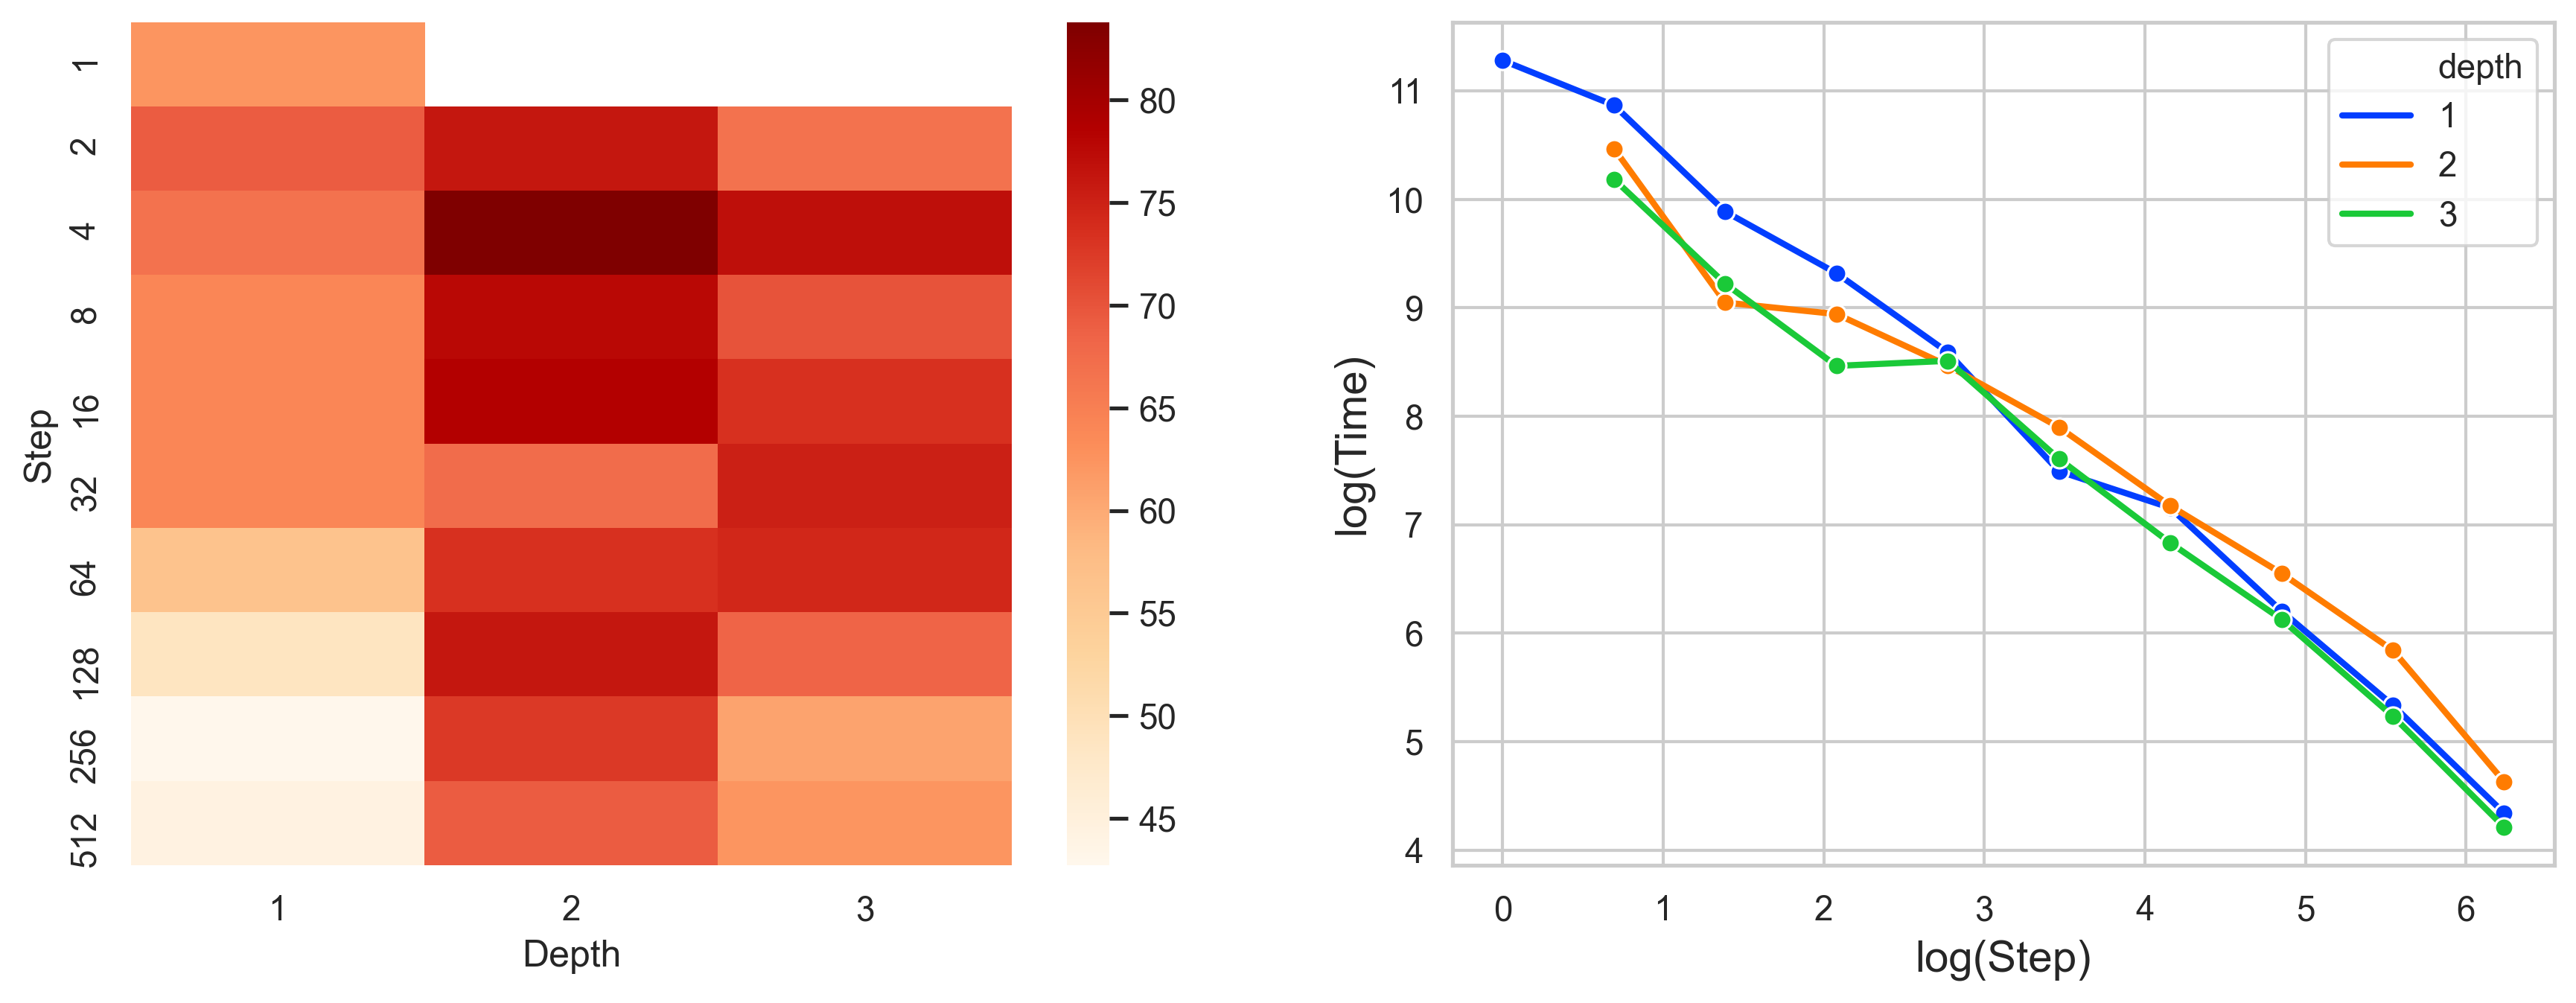
\includegraphics[width=0.95\textwidth]{Images/eigenworms.png}
    \caption{\textbf{Left:} Heatmap of accuracies on the EigenWorms dataset for differing step sizes and depths. \textbf{Right:} Log-log plot of the elapsed time of the algorithm against the step size.}
    \label{fig:eigenworms}
\end{figure}

\input{Tables/eignworms}

See Table \ref{tab:eigenworms}. We see that the straightforward $\mathrm{NCDE}^1_1$ model takes roughly a day to train. Using the log-ODE method ($\mathrm{NCDE}_2$, $\mathrm{NCDE}_3$) speeds this up to take roughly minutes. Doing so additionally improves model performance dramatically, and reduces memory usage. Naive subsampling approaches ($\mathrm{NCDE}^{8}_1$, $\mathrm{NCDE}^{32}_1$, $\mathrm{NCDE}^{128}_1$) only achieve speedups without performance improvements.

See also Figure \ref{fig:eigenworms}, in which we summarise results for a larger range of step sizes.

\subsection{Estimating Vitals Signs from PPG and ECG Data}
Next we consider the problem of estimating vital signs from PPG and ECG data. The data is taken from the TSR archive \cite{MonashTSRegressionArchive} and involves data from the Beth Israel Deaconess Medical Centre (BIDMC). We consider three tasks whereby we aim to predict a persons respiratory rate (RR), their heart rate (HR), and their oxygen saturation (SpO2). This data is sampled at 125hZ with each series having a length of 4000, 7949 training samples, and a dimension of 3 (including time).

We train a model on each of the three vitals sign prediction tasks using a similar approach to the EigenWorms dataset. The metric used to evaluate performance is the root mean squared error (RMSE) loss which is the standard loss considered in the TSR archive. The results over a range of step sizes are presented in table (\ref{tab:bidmc}). The full results over all step sizes, along with a plots analogous to figure \ref{fig:eigenworms} are left to Appendix \ref{apx:results}.

\input{Tables/bidmc}

We find that the depth $3$ model is the top performer for every task at any step size. Whats more, the top performing depth 3 model from each category also significantly outperforms the NCDE$^1_1$ model with a significantly reduced training time. This again illustrates that the increased step size not only reduces training time, but can also improve model performance. We believe this is attributable to the log-ODE model being better at learning these long-term dependencies, as the worst scores of the NCDE$^s_{2, 3}$ models are with step sizes 2 and 4 for all tasks where they are on par (or worse) than the corresponding depth 1 model.

Both experiments give show that the depth 2 and 3 models can not only reduce training times with similar levels of performance, but can additionally result in improved performance over these large steps. 


\section{Limitations}

\paragraph{Number of hyperparameters} Two new hyperparameters -- truncation depth and step size -- with substantial effects on training time and memory usage must now also be tuned.

\paragraph{Number of input channels} The log-ODE method is most feasible for low numbers of input channels, as the number of logsignature channels $\beta(v, N)$ grows near-exponentially in $v$.

\section{Related Work}
There has been some work on long time series for classic RNN (GRU/LSTM) models. \citet{campos2017skip} introduce the `Skip-RNN' model, which extend the RNN by adding an additional learnt component that skips state updates. This reduces the number of computations in the forward pass. However, this model is now not dependent on the within-skip input data. Furthermore, one does not know a priori how many states the model will choose to skip, which can lead to memory difficulties. 

Another approach is hierarchical subsampling as in \citet{graves2012supervised, de2015survey}, which operates over multiple training examples at a time as an input, thus reducing the number of total forward computations. Whilst this method is dependent on all the data, it naively uses the raw data when an appropriate summarisation would be more sensible.

This is rectified in \cite{liao2019learning} where the authors in fact use the logsignature as their summarisation procedure.


However, as is common with all of these models, it describes some some modification of the RNN structure but it has been shown in \cite{kidger2020neural} that the NCDE model subsumes the class of RNN/LSTM/GRU, in that it can model a wider class of functions. Additionally, none of these approaches be solved using ODE methods and thus are not able to utilise the adjoint method, continuous time dynamics, and so on.   


\section{Conclusions}
We have shown how the integral equation from the Neural CDE model can be solved with high accuracy over intervals larger than the discretisation of the data can be solved using the log-ODE method. We demonstrated that this not only enables us to take longer steps over the data whilst retaining model performance resulting in significantly lower training times, but also that this can result in models that achieve better performance over large step sizes than the original model over any step size, including updating the hidden state at every data point. 




\subsubsection*{Author Contributions}


\subsubsection*{Acknowledgements}
JM was supported by the EPSRC grant EP/L015803/1 in collaboration
with Iterex Therapuetics. CS was supported by the
EPSRC grant EP/R513295/1. PK was supported by the EPSRC grant EP/L015811/1. JF was supported by the EPSRC grant EP/N509711/1. JM, CS, PK, JF, TL were supported by the Alan Turing Institute under the EPSRC grant EP/N510129/1.


\bibliography{bibliography}
\bibliographystyle{style/iclr2020_conference}

\newpage

\documentclass{article} % For LaTeX2e
\usepackage{style/iclr2020_conference,times}

% Optional math commands from https://github.com/goodfeli/dlbook_notation.
\input{math_commands.tex}

\usepackage{hyperref}
\usepackage{url}

\usepackage{booktabs}       % professional-quality tables
\usepackage{arydshln}
\usepackage{amssymb}
\setlength\dashlinegap{2.5pt}

\usepackage{graphicx}
\usepackage{subcaption}
\usepackage{rotating}
\usepackage{ifthen}
\graphicspath{ {Images/} }

\newtheorem{theorem}{Theorem}[section]
\newtheorem{lemma}[theorem]{Lemma}
\newtheorem{prop}[theorem]{Proposition}
\newtheorem{proof}[theorem]{Proof}
\newtheorem{corollary}[theorem]{Corollary}
\newtheorem{method}[theorem]{Method}
\newtheorem{definition}[theorem]{Definition}
\newtheorem{example}[theorem]{Example}
\newtheorem{xca}[theorem]{Exercise}
\newtheorem{remark}[theorem]{Remark}

% This file contains lots of tikz stuff
\input{Images/ncde_diagram_script}
\usetikzlibrary{external}

% Tikz network diagram
\tikzset{middlearrow/.style={
        decoration={markings,
            mark= at position 0.5 with {\arrow{#1}} ,
        },
        postaction={decorate}
    }
}
\tikzset{input/.style={black, draw=green!50, fill=green!50, rectangle, minimum height=0.8cm}}
\tikzset{hidden/.style={black, draw=blue!50, fill=blue!50, rectangle, minimum height=0.8cm}}
\tikzset{hidden_square/.style={black, draw=blue!50, fill=blue!50, rectangle, minimum height=3.5cm}}
\tikzset{logsig/.style={black, draw=red!50, fill=red!50, rectangle, minimum height=0.8cm}}


\title{Neural CDEs for Long Time Series via the Log-ODE Method}

% Authors must not appear in the submitted version. They should be hidden
% as long as the \iclrfinalcopy macro remains commented out below.
% Non-anonymous submissions will be rejected without review.

%\iclrfinalcopy

\author{James Morrill \And Patrick Kidger \And Cristopher Salvi  \And James Foster \And Terry Lyons\AND\\[-20pt]
Mathematical Institute, University of Oxford;\\
The Alan Turing Institute, British Library\\[2pt]
\texttt{\{morrill, kidger, salvi, foster, tlyons\}@maths.ox.ac.uk}
}

% The \author macro works with any number of authors. There are two commands
% used to separate the names and addresses of multiple authors: \And and \AND.
%
% Using \And between authors leaves it to \LaTeX{} to determine where to break
% the lines. Using \AND forces a linebreak at that point. So, if \LaTeX{}
% puts 3 of 4 authors names on the first line, and the last on the second
% line, try using \AND instead of \And before the third author name.

\newcommand{\fix}{\marginpar{FIX}}
\newcommand{\new}{\marginpar{NEW}}
\newcommand{\logsig}{\mathrm{LogSig}}
\newcommand{\dby}{\mathrm{d}}
\newcommand{\reals}{\mathbb{R}}
\newcommand{\naturals}{\mathbb{N}}
\newcommand{\restr}[2]{{\left.\kern-\nulldelimiterspace #1 \right|_{#2}}}

\begin{document}


\maketitle

\begin{abstract}
Neural Controlled Differential Equations (Neural CDEs) are the continuous-time analogue of an RNN, just as Neural ODEs are analogous to ResNets. However just like RNNs, training Neural CDEs is difficult for long time series. Training takes impractically long, and models may fail to train. Here, we demonstrate that an existing numerical method for the solution of CDEs -- the log-ODE method -- may in the context of Neural CDEs be used to take integration steps \emph{larger} than the discretisation of the data, whilst depending upon sub-step data through additional terms. Doing so represents making a length/channel trade-off, and is easy to implement with existing tools. We demonstrate efficacy on problems of length up to 17k observations and observe training speed-ups from roughly days to roughly minutes.
\end{abstract}


\input{Sections/1_Introduction}

\input{Sections/2_Methods}

\input{Sections/3_Experiments}

\input{Sections/4_Limitations}

\input{Sections/5_RelatedWork}

\input{Sections/6_Conclusions}


\subsubsection*{Author Contributions}


\subsubsection*{Acknowledgements}
JM was supported by the EPSRC grant EP/L015803/1 in collaboration
with Iterex Therapuetics. CS was supported by the
EPSRC grant EP/R513295/1. PK was supported by the EPSRC grant EP/L015811/1. JF was supported by the EPSRC grant EP/N509711/1. JM, CS, PK, JF, TL were supported by the Alan Turing Institute under the EPSRC grant EP/N510129/1.


\bibliography{bibliography}
\bibliographystyle{style/iclr2020_conference}

\newpage

\input{Sections/Appendix/main}

\end{document}


\end{document}


\end{document}


\end{document}
